%%% File encoding: UTF-8
%% äöüÄÖÜß  <-- no German Umlauts here? Use an UTF-8 compatible editor!

%%% Magic comments for setting the correct parameters in compatible IDEs
% !TeX encoding = utf8
% !TeX program = pdflatex 
% !TeX spellcheck = en_US
% !BIB program = biber

\documentclass[master,english]{hgbthesis}
% Permissible options in [..]: 
%   Type of work: diploma, master (default), bachelor, internship 
%   Main language: german, english (default)
%%%----------------------------------------------------------

\RequirePackage[utf8]{inputenc}		% Remove when using lualatex or xelatex entfernen!

\usepackage[graphicx]{realboxes}
\usepackage{rotating}
\usepackage{array}

\makeatletter% Set distance from top of page to first float
\setlength{\@fptop}{5pt}
\makeatother

\graphicspath{{images/}}    % location of images and graphics
\logofile{logo}				% logo file = images/logo.pdf (use \logofile{} for no logo)
\bibliography{references}  	% name of bibliography file (references.bib)

%%%----------------------------------------------------------
% Title page entries
%%%----------------------------------------------------------

%%% Entries for ALL types of work: --------------------------
\title{CodeSpeech: An Eclipse Plugin for \\Java Programming by Voice }
\author{Łukasz Strzelecki}
\programname{Mobile Computing}
\placeofstudy{Hagenberg}
\dateofsubmission{2019}{08}{26}	% {YYYY}{MM}{DD}

%%% Restricted publication license instead of CC (master only):
%\strictlicense

%%%----------------------------------------------------------
\begin{document}
%%%----------------------------------------------------------

%%%----------------------------------------------------------
\frontmatter							% title part (roman page numbers)
%%%----------------------------------------------------------

\maketitle
\tableofcontents

%\chapter{Preface}





 	% preface is optional
\chapter{Abstract}

As other computer users, some of the programmers develop Repetitive
Strain Injuries (RSI) or for other reasons have troubles with
using keyboard and mouse. Not to mention people whose disabilities
prevent them from taking up a work as a programmer in the first
place. With Speech Recognition (SR) systems getting better, another
way of interacting with computers opens up. Programming,
however, because of its specific syntax cannot be successfully
done using available, commercial SR tools. Therefore an idea for a new system for programming by voice arose. That gave birth to a prototype called CodeSpeech, developed as an Eclipse IDE plugin for Java programming language created especially for this purpose. This paper deals with the whole process behind its creation, including requirements definition, design of architecture, description of utilized tools, implementation phase and ends with a first evaluation of the initial iteration's product, deriving conclusions, discussing them and proposing certain solutions for future development. The evaluation compares the new programming method using CodeSpeech with the standard way of programming using mouse and keyboard by recreating a
given sample program and measures the completion time, as well as the use of peripheral devices. In addition, Command Error Rate (CER) metric was measured during the test. The conducted experiment showed that the prototype is around four times slower than the regular programming method, it decreases however the time of mouse and keyboard usage to 37,6\%, distance traveled by the cursor to 17,4\%, keystrokes required to 29,9\% and the number of clicks and doubleclicks to 20\% and 5\% respectively. Calculated CER was 29,5\%, meaning there is room for improvement. The result shows that in the current state CodeSpeech is not feasible to replace mouse and keyboard due to the time it requires for program completion, nonetheless it shows that the potential exists, and with further program development a time might come when its performance becomes competitive to the standard means of programming while keeping all of the benefits of contactless programming.


%\include{front/kurzfassung}

%%%----------------------------------------------------------
\mainmatter          			% main part (arabic page numbers)
%%%----------------------------------------------------------

\chapter{Introduction}
\label{cha:Introduction}

% description of the problem, why is it important to address it, what solutions I proposed and how well did it work

This thesis deals with a CodeSpeech project - an Eclipse IDE plugin whose goal is to present an alternative for standard means of programming, which is nowadays exclusively done via mouse and keyboard. The prototype allows using programmer's own voice in order to create basic programming structures in Java language and perform basic operations in the integrated development environment. The paper starts with an explanation of motivation standing behind the idea of introduction of such tool and describes the problem that it tries to solve. Then the document continues with a presentation of a whole thinking, creative and practical process of architecture design and implementation phases, followed by system's evaluation and discussion of results to finally finish with a summary of what has been done, what are the lessons learned throughout the whole experience, stating arising conclusions and potential enhancement possibilities to be performed in the future.

\section{Problem}
Computer science studies (or related topics), as the name suggests, involve the use of computers. This includes an enormous amount of hours spent sitting in front of a desk. According to research done by Schlossberg et al. on engineering graduate students,
\begin{quote}\begin{english}
    During the first year, 80\%
    used a computer more than 20 hours per week and by the fifth year this had increased to
    95\%. Those reporting greater than 40 hours of computer use per week increased each
    year in graduate school, beginning with 34\% of participants in the first year and
    increasing to 56\% in the final years of study. \cite{Schlossberg2004} 
 \end{english}\end{quote}
Very often during the late period of studies, an internship or a temporary job in the field is taken up by a student which increases the amount of time spent that way even further. 

 Although results of existing studies on direct relation between usage of computer and severe health conditions vary, many of them involve long term computer users that report pain. Schlossberg et al. confirm in their research done on randomly sampled 206 Electrical Engineering and Computer Science graduate students that \textit{hours of computer use per week is associated with an increased risk of persistent or recurrent upper extremity or neck pain}  \cite{Schlossberg2004}. Lassen et al. performed a year lasting study on 6943 computer operators which ended in a positive association between self-reported mouse and keyboard times and elbow and wrist/hand pain \cite{Lassen2004}. Their later study, however, did not confirm that the use of mouse and keyboard are predictors for persistent and severe pain \cite{Lassen2005}. Chang et al. state that their data \textit{suggest a potential dose–response relationship between daily computer usage time and musculoskeletal symptoms} \cite{Chang2007}. Brandt et al. conclude their study with the statement that \textit{mouse use is associated with an increased risk of moderate-to-severe pain in the neck and right
shoulder, and an association with tension neck syndrome is possible} \cite{Brandt2004}.
 
 Many of the problems are suspected to be caused by repetitive movements that working with peripheral devices such as mouse and keyboard requires. These symptoms started to be known under an umbrella term ``Repetitive Strain Injuries'' (RSI). This topic is broadly described by Van Tulder et al. \cite{VanTulder2007} and Yassi \cite{Yassi1997}. Another factor that supposedly has a negative effect on health is sedentary lifestyle, inevitable in any kind of desk work (so also with computers). Tremblay et al. analyse this problem deeper \cite{Tremblay2010}. Van den Heuvel et al. \cite{Van2007} and Walker-Bone et al. \cite{Walker2005} prove that physical injuries can result such negative consequences as increased amount of absence from work as well as decreased productivity at work. Aforementioned issues do not touch only computer scientists, but any profession that is the use of computers on a daily basis such as office workers, graphic designers \etc  Main problems that are frequently reappearing are neck, upper extremity pain (shoulder, elbow, wrist and hand), Carpal tunnel syndrome, lower back pain and similar musculoskeletal symptoms. 
 
\section{Motivation}
The author of this thesis himself fell victim to some of those issues and after many years of studies developed chronic pain in lower back, neck and recently also shoulders. The pain began to be very problematic not only in times of working on a computer, but also in everyday life. That was the main reason for the idea of creating a new way of interaction with computers with emphasis on programming, which is an occupation of the author.

Progress in certain fields of science such as Machine Learning and Big Data opens up new possibilities that previously could only be imagined. Speech Recognition (SR) is one of the most ``recent'' technologies that benefit from these fields of science and start to very popular. Nowadays SR is used by many and it takes many forms. Be it Amazon's Alexa, Apple's Siri, Microsoft's Cortana, Google's Assistant and more, they all allow for voice control over devices. Speech Recognition is being utilized in smartphones, cars and automated households. It is this technology, that the author saw as the one that brings in 
a new opportunity for alternate way of programming. Unfortunately, available commercial tools are not suitable for this task. Those are mainly created to write text in national languages and perhaps to recognize special commands for system control. Programming languages, however, because of their specific syntax cannot be successfully transcribed by them. The grammar of many programming languages requires awkward use of brackets, parentheses, semi-colons and other punctuations. Therefore a need for an adhoc solution appeared, a tool that could solve the problem of awkward code formatting and enable programming by voice.

Such a tool would not only help to prevent the development of upper extremities pain linked to the use of mouse and keyboard, but also free the programmer from the need of sitting in front of the desk. With nowadays broadly available wireless microphones, the potential software developer could move away from a workstation and take more comfortable position, perform stretches, simple exercises or just walk around the room giving them the opportunity for much more active and healthier lifestyle than it has been possible up to this point. 

Going further with this idea, another potential usage was found. There are people with more severe physical conditions than just chronic pain, namely upper body impairments or a paralysis. The state of such people obviously makes it impossible for them to use a standard way of interacting with computers and thus excludes them from taking up a potential occupation as a programmer. Different tools were created to allow disabled people to utilize computers, none yet specifically designed for coding. How great would it be to enable some people with brilliant minds yet  limited in their bodies to take a job as a programmer and to be as productive as completely healthy person. This could improve their lives in many ways. It could give them purpose and a way of greatly contributing to the society by development of the new software. That obviously would lead to the improvement of their material situation, in result making it easier to pay for many specific needs these people have. 

It seems that, even though such a tool might not have a big impact on the world, it still can prove useful to many existing programmers suffering from occupational injuries and at the same time provide a new group of programmers arising from physically impaired people to fill the ever growing needs of the market.

\section{Goal}
The goal of the project is to create a software that will allow programming using voice. The tool should be somehow compatible with an already existing Integrated Development Environment (IDE) and should utilize available speech recognition engine. Creating new, specific SR engine or programming environment from scratch are not the topic of this thesis, but rather combining different, already existing tools and forming a completely new product. 

\section{Overview}
This section gives an overview of the content of this thesis by briefly describing each subsequent chapter and what can be found in it.

The second chapter titled \textit{Related work} focuses on description of several existing studies related to the topic of voice programming. Most of the selected documents present similar programming by voice projects. These projects are briefly presented in this chapter and compared to the subject of this thesis. Additionally, other research that is not based on any system but is still relevant is mentioned.

The third chapter is titled \textit{Tools} and there one can find description of various software that have been used in order to complete the CodeSpeech project. The first section is dedicated to Eclipse IDE, the second to its extension for plugin development, the third one is focused on three different speech recognition technologies: belonging to CMUSphinx family of open-source tools PocketSphinx and Sphinx4, and a commercial Google Cloud Speech-to-Text service. The end of this section deals with performance comparison thereof. The last section describes a parser software called ANTLR.

Right after that there is \textit{Method} chapter, which is a place where functional and non-functional requirements are stated, use cases defined and the design of architecture is presented. 

The \textit{Implementation} chapter as the name suggests is fully devoted to the process of implementation. It describes the structure of the project based on previously defined architecture, presents the most important classes and interfaces, guides through the workflow of a working cycle to finally discuss some of the interesting features and walk through the process of adding new functionality backed by an example.

The next on the list, \textit{Evaluation} chapter deals with the test that was undertaken on the finished prototype. The approach is being described in detail to leave no doubts about how it was performed. The metrics of interest are explained together with the way they were recorded. Then there is a presentation of the results followed by the discussion of the received scores and what do they mean. In the end, a couple of ideas that arose during or after the evaluation as to how the project can be improved are presented.

Finally, the \textit{Conclusions} chapter summarizes what has been done up to this point. It goes through the statement of the initial problem and how the proposed solution potentially solves it. Then it describes a way the goal was achieved with thinking, creative and practical process behind it, as well as the experience gained throughout the course of development. An objective evaluation of the system overall, how well does it serve its purpose and satisfies initial requirements is given. The chapter and therefore the whole thesis concludes with the statement on the future plans for the project and its continuation.


\chapter{Related work}
\label{cha:RelatedWork}

This chapter focuses on a short summary of similar projects that have been done in the past and comparing them with the one that is the main topic of this paper. After reading this chapter it should be clear how this project is different from others, what is innovative and what is done in a similar matter. At the end, other important studies related to the topic of programming by voice are discussed. 

\section{VoiceGrip \& VoiceCode}

Désilets et al. describe VoiceCode as ``Innovative Speech Interface for Programming-by-Voice'' \cite{Desilets2006}. After reading their paper and watching an online video  presenting its functionality \cite{VoiceCode2007} it does seem that this is the most complete software in comparison with others. It is not a surprise, seeing how it has been developed through many years, evolving from earlier VoiceGrip project described by Désilets \cite{Desilets2001}. Désilets et al. see the problem in the use of existing SR tools for the purpose of writing code and put focus on providing a way to use more natural utterances. The earlier document has more content and goes through the tasks with which programmers have to deal with in their everyday job and what problems occur in performing them while using SR. VoiceGrip already handles well many of those tasks. The main difference between the two, is that in VoiceGrip, so called pseudo code is being written down word by word and is translated to native code by the Code Translator only when programmer runs it. In VoiceCode the translation is done in real time. Another big modification introduced in the new version was an addition of error correction. It provides two types of error correction: \textbf{Not What I Said}  - when VoiceCode did not recognize the utterance properly and \textbf{Not What I Meant} - to address situations where recognition was correct but translated to the wrong code. This two fold system does not only allow for an easy modification of a mistake but also lets the system to adapt and avoid same mistakes in the future. Both projects allow code navigation. Because it is not clearly stated in what form VoiceCode comes, it is assumed that it is a similar tool as its predecessor, meaning that it can be utilized with different SR systems, such as Dragon NaturallySpeaking, and it can be used by different programming editors, like \eg Emacs. It requires, however, an application of few macros before use. CodeSpeech on the other hand was built as a plugin to commonly used, free of charge IDE - Eclipse and uses built-in SR. It is therefore neither cross SR, nor cross editor. This can come as an advantage or disadvantage with the relation to the other two. First, it is limited only to one IDE and thus cannot be used with another one, possibly preferred by a potential programmer. On the other hand, no special configuration is needed and once the program with plugin is installed, it enables programming by voice with a single click. Another advantage over the aforementioned tools, coming from the choice of a specific, broadly developed IDE is that it is easy to enhance CodeSpeech to execute every single command that exists in Eclipse environment, such as adding breakpoints, compilation, debugging \etc, as well as calling functionality from other plugins, if those are available in the current instance. The software that is the topic of this thesis is just a prototype, therefore it lacks many of the important features that the programs developed by Désilets and the team have, such as sophisticated error correction or transferability across programming languages (VoiceCode can enter specific syntax depending on file extension while CodeSpeech is strictly developed for Java). Many of the provided functionality like local navigation, is still implemented in a limited manner. By the time of writing this thesis neither VoiceGrip nor VoiceCode were available online to try them out.

\section{VocalProgrammer}
Arnold et al. \cite{Arnold2000} have designed a generator of voice recognition syntax-directed programming environments called VocalGenerator. It takes as input context-free grammar for a programming language and a voice vocabulary for that language. Because of that it supports different languages such as Basic, C, C++, Java etc. The authors argue that because of its syntax-directed editing two major capabilities are provided that the standard text editors do not include: navigation and selection. Having that, the authors decided to create another project based on VocalGenerator called VocalProgrammer. This project was supposed to be using using Dragon NaturallySpeaking and Microsoft Visual C++ with focus on Java programming language because its full documentation is available online for free. This tool would require a user to have purchased Dragon NaturallySpeaking Professional Version. Because of no further mention of this project it is assumed that it has never came to a conclusion. 

VocalGenerator is a completely different tool than CodeSpeech. Deriving from description, however, it seems like a similar tool could be developed by it. VocalProgrammer was supposed to be such a tool. It was to be based on Java similarly to CodeSpeech. CodeSpeech does not require any external SR engine as VocalProgrammer would. VocalProgrammer lacks modularity that Eclipse provides, therefore scalability of its functionality seems limited. VocalGenerator allows creation of many editors for different languages, which is a big advantage.

\section{VocalIDE}
VocalIDE is a prototype created in JavaScript created by Rosenblatt et al. \cite{Rosenblatt2018}. It is a web application that allows writing source code using a set of vocal commands. It records and recognizes users' speech using WebkitSpeechRecognition currently available in browsers such as \eg Google Chrome, and rule-based syntax parser. It allows text entry, navigation, text selection, replacement, deletion and snippet entry. Text entry works like in a regular speech recognition program meaning each symbol character has to be explicitly given (``type open parenthesis i space less than space one close parenthesis to enter (i < 1)''). It makes it rather inconvenient to program by voice and is something that CodeSpeech successfully avoided. It is an interesting idea to create such a tool as a web application, which has an advantage of the fact that it can be accessed from everywhere where any kind of computer with a browser is available (which nowadays is rather taken for granted). Requirement for the Internet can be a disadvantage at the same time. CodeSpeech is strictly dependent on a specific program (Eclipse), which has to be installed on a computer first. As for Internet access, for now it is a requirement since it is preferred to use Google Cloud Service, which provides better recognition. Both programs are based on rule-based syntax parser.

Local navigation in both projects is done in a similar manner - the user can say ``go to line'' with a number to jump to a specific line. VocalIDE has developed text selection by word as well as replacement which is something that CodeSpeech lacks so far. Undo operation and smart snippet entry (entering ready code block) are both available in CodeSpeech. Interesting idea presented in this paper is Context Color Editing. Instead of moving the cursor to left or right by one character, nearby words are highlighted in different colors. Saying that color's name moves the active selection to the respective word.

VocalIDE was developed based on the results of research that used Wizard of Oz method. The system was evaluated during the study performed on eight impaired participants. Both researches, as well as the design of a prototype were mostly focused on navigation and selection in Java code.


\section{SPEED: Speech Editor}
SPEED is a program editor described by Begel \cite{Begel2005} which together with program analysis framework called Harmonia \cite{Boshernitsan2001} creates a system embedded in Eclipse IDE. It allows for code creation and edition together with high-level program manipulations like refactoring. To translate voice commands to code it uses SpokenJava - a semantically isomorphic dialect of Java that is more natural to be verbalized \cite{Begel2004}. It allows to replace phrases like ``open braces'' with ``begin class'' in order to create an open bracket after class declaration. That seems to be a big difference between CodeSpeech and SPED, namely, CodeSpeech uses context-free grammar, which once recognized, creates a specific programming construct without the need of handling parenthesis, brackets or explicit starting or ending of these constructs. In order to help people with voice input Begel's project mentioned adding a specific spoken feedback system that would make its use easier to speak proper phrases. Because of strict dependency on grammar, CodeSpeech requires a similar feedback system to help users in learning of the commands for smooth usage. Additionally, a special search and selection tool was being developed for SPED, to help with finding a specific words based on phonetics without spelling a word precisely - similar system is needed for CodeSpeech.

The SPEED system has quite sophisticated feature to handle and support ambiguities through the syntactic phases of program analysis, as well as support for combination of commands and code. It is not clear at which stage of development the project has ended because no further studies on it were found. Just like the rest of the above mentioned projects, this one was not available at the time of writing the thesis. 

\section{NaturalJava}
Shinde describes an interface for programming called NaturalJava \cite{Shinde2017}. It allows entering English sentences as input which produce Java source code as output. It uses information extraction techniques to generate so called case frames that classify key concepts of the sentence. The case frames are then used to modify Abstract Syntax Tree (AST) accordingly. This is the first project (from above mentioned) that uses manipulation of AST rather than being simply text based. Same method is used in CodeSpeech, where specific commands result in creation, deletion or modification of AST nodes. NaturalJava has a very interesting way of interpreting English sentences, which seems to get triggered based on detected keywords such as ``iterates'' in sentence ``create a for loop that iterates from 1 to 5''. CodeSpeech analyses provided utterances via parsed tree walking, and similarly triggers specific actions based on detected keywords. The biggest difference is that NaturalJava does not utilize any speech recognition tool, utterances are to be typed in order to generate code.

\section{CodeTalker}
Snell and Cunningham propose CodeTalker project\cite{Snell2000}. The program was developed as a standalone editor that allowed simple source code creation (in Java) such as definition of a class, function, variable, constructs like for, while loops and switch statements. The editor was created very carefully, iteratively with each version being evaluated in terms of Human Computer Interactions (HCI). The paper also mentions the possibility of creating HTML code.
It contains many useful features, such as replacement of previously defined spoken keywords with text (\eg saying class will insert \texttt{class \{ 
\textbackslash n \}}) and addition of completely new, personal replacements via dialog wizard. It also has an option to highlight syntax, as well as to add specified keywords to be highlighted. Example of spoken input is ``public class my class, braces, private void my function, open brackets, close brackets, braces, count equals my variable, semi-colon''. As can be seen, the punctuation has to be explicitly stated which is something that CodeSpeech wanted to avoid by all means. This, however, allows the CodeTalker to detect if a construct is a class, a variable or a function. In many situations the end of a spoken utterance has to be marked by saying either ``tilde'' to invoke command or `circumflex'' to cancel it. CodeTalker provides a way for entering a word that is reserved as a keyword, which is a common problem in command based systems. Main differences are dependency on other tools and functionality. While CodeSpeech is a plugin that obviously requires Eclipse IDE, CodeTalker is a standalone tool. It requires, however, an external speech recognition software. The former makes operations on AST rather than text, and allows more operations than just creating constructs with specific names but also provides a way to utilize built into Eclipse commands that are important part of the programming, such as compilation and debugging.

\section{Vocal}
An interesting idea of bringing programming by voice to smartphones was brought by Islam et al. \cite{Islam2018}. ``Vocal - a voice based code generator'' is an Android application that enables creation of code by voice. It uses Google Cloud Speech API (similarly to CodeSpeech) as it turned out to be the most accurate from total of free that they have tested out. Only creation of simple structures such as integer or character variables, arrays, method definitions, while and for loops and printing to console is possible in this program. The generated source code is of Java programming language. This software requires an Internet connection to exchange data with the cloud for the feature of compilation on the server. Database is used for storing text files. Although mobiles are not yet suitable for programming, the idea itself is curious. The use of smart devices could potentially make it possible to program conveniently in any place and taking into account Internet accessibility in the world it sounds feasible. Obvious difference between this project and the CodeSpeech is targeted device.

\section{Voice and Gesture Development Environment}

Voice and Gesture Development Environment (VGDE) is an interesting project presented by Bouse \cite{Bouse2017}. It combines together an idea of voice and hand gesture control of the system. Voice commands are used to create and edit code, navigate through it and interact with the program. Gesture commands on the other hand are used only for editing and navigation in the file. This provides a possibility of mixing two methods together as they run in concurrent threads. The author recommends that to achieve the best results one to two second breaks should be done between the commands. This probably makes programming with VDGE quite slow, while in given example ``Bar Equals One Okay'' there are four commands, therefore four breaks are needed. This commands would produce code ``bar = 1;''. The evaluation of VDGE, however, did not measure the system's execution time. To be fair, CodeSpeech also requires around two seconds break between commands as this is the average time of recognition. The difference is, that in the example mentioned above VDGE's four commands correspond to one command in CodeSpeech. \\
Voice recognition is performed by Microsoft Speech and gesture recognition requires external device, namely Leap Motion. Leap Motion is a small device that can be placed between the user and a keyboard. It tracks hands with discrimination of fingers. VDGE unlike CodeSpeech is a standalone development software. Its code manipulation is done on text and does not perform AST operations as CodeSpeech does. It does, however, allow for more detailed navigation in the code. VDGE's targeted programming language is Java, as well as it is of CodeSpeech. Commands are based on grammar and parsed in a similar manner in both programs. Both tools are limited as to the complexity of program that can be created using them, although they do possess the potential for extension.

\section{Voicecode.io}
At the time of writing the thesis one of the most recent programming by voice tools being created was Voicecode.io. The author of the tool is Ben Meyers. The tool on the official website is described as 
\begin{quote}
    \begin{english}
    a concise spoken language that controls your computer in real-time. When writing anything from emails to kernel code, to switching applications or navigating Photoshop - VoiceCode does the job faster and easier. 
    
    VoiceCode is different from other voice-command solutions in that commands can be chained and nested in any combination, allowing complex actions to be performed by a single spoken phrase \cite{Voicecode.io2017}.
    \end{english}
 \end{quote}
From the description it can be concluded that the tool is not a programming tool per se but a general software for system control and it is de facto that. To allow system control Voicecoe.io integrates Dragon NatruallySpeaking SR technology and SmartNav for mouse-free control of the cursor. SmartNav uses a small device that sends infrared waves which reflect from a small pin that can be attached to the baseball cap. This allows for tracking position of the head and moves the cursor accordingly. It is a similar solution to eye tracking technology. The general idea for hand-less system control is great by itself, however what is at the point of interest for the sake of this thesis is its ability to write code. On one of the videos available on official website there is a presentation of an example. The code being written is in JavaScript. Written code is only three lines long and is being written fairly fast. Unfortunately, commands that are spoken to achieve this goal sound nothing like natural English sentences. It is hard to follow and understand which command does what and probably a lot of learning has to be done in order efficient. There is a second video showing writing a script in Ruby, meaning that Voicecode.io is not limited to one programming language, perhaps because it simply writes dictated text (so also punctuations). Currently Voicecode.io supports only MacOS and is constantly under development.

\section{SOPE and ELDI}
An interesting paper written by Bettini and Chin \cite{Bettini1990} comes from year 1990. They describe inside the first results from a research project on man-machine interaction based on speech. SOPE (Speech Oriented Programming Environment) was a project of which the goal was to create programming interface steered by voice. At the beginning the main focus was put on debugging process. In order to do that, IBM's Tangora speech recognition was used and created by them ELDI (English Language Debugger Interface) prototype based on Augmented Transition Networks (ATN). Their goal was to use natural English sentences based on grammar, which at the beginning was quite strict. The restricted vocabulary was up to 60-70 entries. The basic concept they presented is very similar to current solutions, yet at that time as the authors conclude, speech recognition technology was not good enough for this kind of tool to be productive.

\section{Problem of speaking code}

Begel \cite{Begel2005}, Arnold et al. \cite{Arnold2000} , Désilets \cite{Desilets2001} and authors of other previously mentioned papers described problems related to the programming by voice. One of the biggest issues is the fact, that source code is known only in written form and there is no unified way to read it. Every programmer, when asked to read code out loud, has a specific way doing so. Analogically the same problem occurs when the program is supposed to be spoken and then translated into source code as it happens to be with programming by voice. Hermans et al. \cite{Hermans2018} examined vocalization of code on group of novices: ten Dutch high school students that received twenty hours of Python lessons. In the end they did confirm that an issue exists, proposing that a standardize code phonology should be developed in the future. This could not only, as it is stated in the document, help to teach and learn programming, in pairwise programming, but speech recognition based development would benefit as well because each system of that kind could perform the same operations using the same spoken phrases. 

Rodriguez-Cartagena et al. \cite{Rodriguez-Cartagena2015} also make this realization and propose a vocabulary and grammar to help in programming by voice in any C-based language. In order to evaluate, it they performed a study on programming community to receive feedback. 
The programming community consisted of random senior students and faculty members of the Computer Science and Computer Engineering Departments at the Polytechnic University of Puerto Rico and the University of Puerto Rico Río Piedras. This was supposed to be an initial phase for Kavita project, however at the time of writing this thesis the website of the project was unavailable.

\section{Summary}
CodeSpeech has certain commonalities with some of the previously mentioned projects, other things it does different, and certain good ideas could still be used in the future. It was decided for CodeSpeech to mainly perform AST operations rather than simply working on strings of text. This should give better control over the program structure \eg when a whole block is to be copied or deleted, or a child node to be replaced without the need of text selection which in the case of voice control might be clumsy. From above mentioned projects only NaturalJava used the same approach. In the current state CodeSpeech consists of a built-in speech recognition system, while many other works such as VoiceCode or VocalProgrammer use external tools like \eg Dragon NaturallySpeaking. In most cases these tools require an additional purchase from users. The initial idea of CodeSpeech was to be free of charge and therefore integrating an open-source SR tool seemed more viable. Additionally, there exists a possibility to adjust such a tool for higher performance in specialized tasks. The program might be, however, extended at some point to allow external software. CodeSpeech similarly to SPEED is integrated into Eclipse IDE and that makes it more than just a program to create code, but provides a way to expand and use all the functionality of a complete programming environment. Similarly to other works CodeSpeech uses grammar for commands. This might be a bit limiting solution, although it is the easiest to implement. An alternative would be to use a special language analysis tool like it was done in NaturalJava or SPEED. Maybe in the future such a software will replace grammar-based approach, but only if it turns out that it allows for control with more natural sentences. CodeSpeech could greatly benefit from better error correction with automatic ability to improve the results in a manner of VoiceCode. A very interesting idea to integrate usage of gestures was given in VGDE project and perhaps one day it will become a focus of CodeSpeech extension, possibly together with the idea of a different representation of the code (rather than standard text form). Many other aforementioned features have not been integrated due to time limitations but are considered for the future.

\chapter{Tools}
\label{cha:Tools}

In order to create the CodeSpeech prototype, multiple different tools were combined together. Because this project was developed as an Eclipse plugin, IDE itself and Plug-In Development Environment (PDE) are used as a development platform. For speech recognition two different toolkits were tested, namely open-source CMUSphinx (in two versions - Pocketsphinx and Sphinx4) and a commercial Google Cloud Speech-to-Text. For analysis of recognized phrases against the grammar file ANTLR parser was utilized. This chapter will introduce and briefly describe each of the aforementioned tools.

\section{Eclipse}

Eclipse is free of charge, open-source Integrated Development Environment. Eclipse is mostly written in Java and primarily used for developing Java applications, although it also allows development in other programming languages such as languages from C family, Python, PHP, JavaScript etc. via plugins. The Eclipse Public License (EPL) is the fundamental license under which Eclipse projects are released. The initial launch was in November of 2001. It can be used at any of the most popular operating systems, such as Linux, Windows, Mac OSX, UNIX. The exemplary view of Eclipse IDE can be seen in Fig. \ref{fig:eclipseIDE}.

It was selected as a development tool and the target platform for three main reasons among others. The first one being, the knowledge of and familiarity with the environment, which the author of this thesis gained during the many years of its use. The second is the fact that Eclipse is easily extendable via plugins (more on that later), therefore it seemed plausible to create an extension for it, especially because it provides a special set of tools that assist in the development of extension (described in the next section). Finally, when doing research about the potential development platforms it turned out that Eclipse JDT API contains all the necessary tools for Abstract Syntax Tree manipulation, which sounded like a perfect way for source code creation from within the program.

\begin{figure}
    \centering
    \fbox{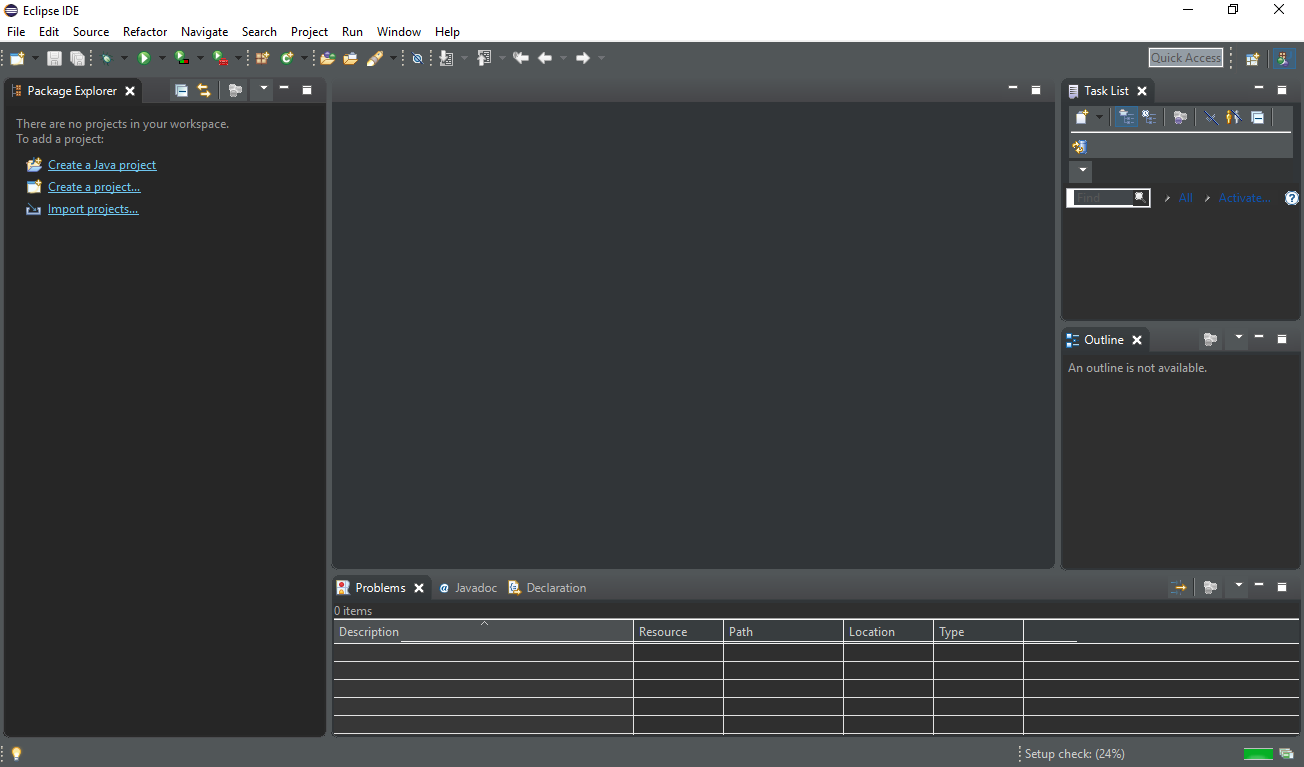
\includegraphics[width=0.8\textwidth]{images/EclipseIDE.png}}
    \caption{Eclipse IDE.}
    \label{fig:eclipseIDE}
\end{figure}

\section{Eclipse PDE}

As mentioned before, Eclipse is mostly known as an IDE. According to Wayne Beaton of Eclipse Foundation \cite{Beaton2013}, however, it was never intended to exclusively be one. It was developed to provide a platform unto which different tools could be integrated. Therefore in fact the core of Eclipse has small functionality by itself and the rest of the tools that are nowadays so broadly used are attached via plugins. That means, Eclipse is designed to be easily extendable. Because of its nature, Eclipse is a perfect tool to be used as a base for general purpose applications. These rich client applications, as well as, plugins for Eclipse core can be developed in Eclipse itself through the use of Plug-in Development Environment (PDE). Once PDE is installed it is enables creation of a new plugin project. The project requires a proper set up at first. Eclipse plugins are based on Open Service Gateway Initiative (OSGi) bundles \cite{Rouse2011}. OSGi is used to manage them in Eclipse application. A plugin must contain a manifest file (\textit{MANIFEST.MF}) with valid OSGi headers for name and version (similarly to Maven). Manifest file is extremely important. It describes the content of a plugin necessary for Eclipse during run-time, such as dependencies, classpath, what is exported \etc Information about the build is held in \textit{build.properties} file. Modular nature of plugins allow them to use other decoupled elements and to be used by other elements as well. This is done by so called extensions and extension points. An extension is \eg a UI element that runs a specific command (which is an extension by itself). CodeSpeech has one UI extension added to the menu - a toggle button that switches the listening on or off. These are managed by another file, namely \textit{plugin.xml}. PDE provides a full featured editor for modifying all three files: \textit{MANIFEST.MF}, \textit{build.properties} and \textit{plugin.xml}.

Once everything is set up, development is focused around a class called the \texttt{Activator}. It is the starting point of any plugin. \texttt{Activator} class extends the \texttt{Plugin} and it is responsible for other classes. The class is initialized whenever any member of the plugin is referenced.

To familiarize the reader with the plugin development using PDE a small example is presented below. The example is explained in detail through the description of the process together with screenshots. The plugin consists of a single toolbar button which displays a message after being clicked. 

\subsection{Necessary software}

As it was mentioned before, the first thing needed is an instance of Eclipse IDE installed in the computer. Eclipse can be downloaded from the official website \footnote{https://www.eclipse.org/eclipseide/}. After that, an enhancement of PDE has to be integrated into the IDE. This can be done via Eclipse Marketplace, accessible from within Eclipse itself, through its menu (Help -> Eclipse Marketplace). In addition to that, yet another software has to be installed, namely Eclipse RCP Target Components. This can be done also through IDE's menu (Help -> Install New Software...). Fig. \ref{fig:eclipseSoftware} show how the corresponding download windows look like. After all of these steps are done, the environment is ready to create a plugin.

\begin{figure}[hbt!]
\centering\small
\begin{tabular}{@{}c@{\hspace{6mm}}c@{}} 
  \fbox{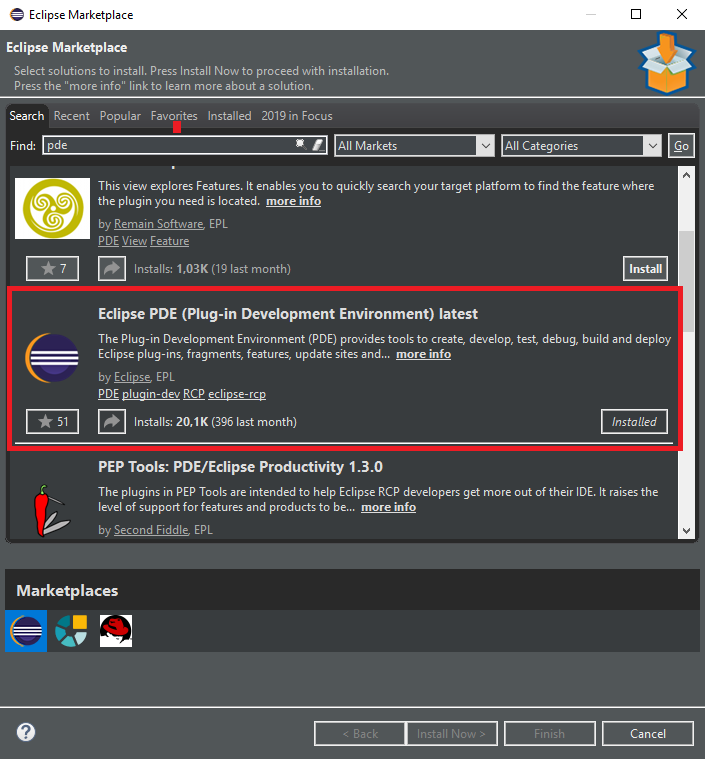
\includegraphics[height=6cm]{images/Tutorial1.png}} &
  \fbox{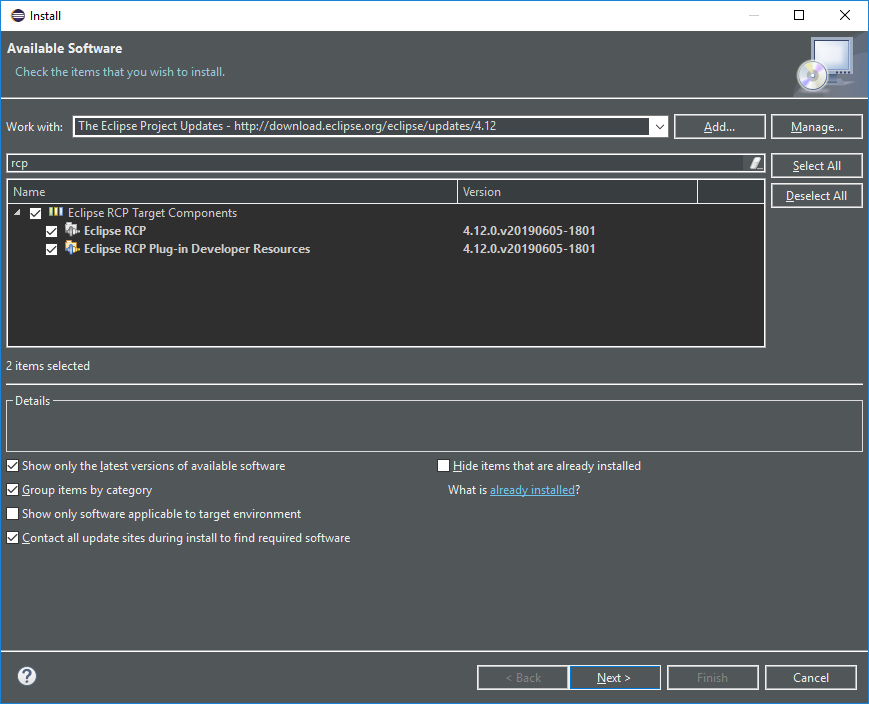
\includegraphics[height=6cm]{images/Tutorial2.png}} 
\\
  (a) & (b)
\end{tabular}
\caption{ Eclipse Marketplace window for PDE donwload (a) and software installation window with Eclipse RCP Target Components Software (b) }
\label{fig:eclipseSoftware}
\end{figure}

\subsection{Project creation}

A plugin can be created in a similar manner as any other type of a project. A creation wizard leads the user through the setup process. The wizard can be opened using menu (File -> New -> Other...). In the pop up window a \textit{Plug-in project} can be selected under the \textit{Plug-in Development} directory. The next consecutive wizard's windows allow for setting up things like plugin's name, id, version as well as setting an \texttt{Activator} and a couple of other options. The last page gives an opportunity to select one of a few plugin templates which comes with some predefined structures. In this example no template is used. Fig. \ref{fig:pluginWizard} shows the sequence of previously mentioned steps.

\begin{figure}[hbt!]
\centering\small
\begin{tabular}{@{}c@{\hspace{3mm}}c@{}} 
  \fbox{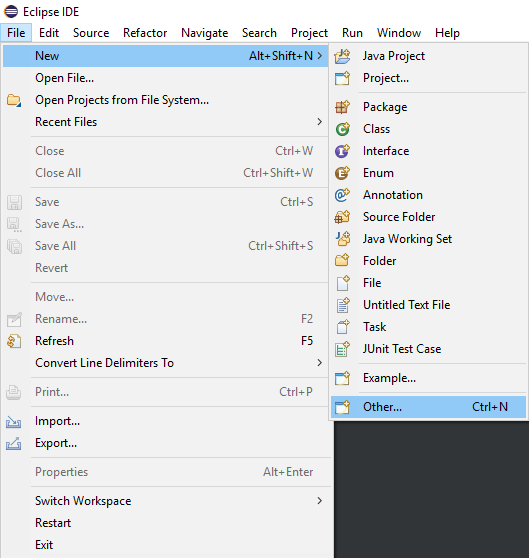
\includegraphics[height=5.5cm]{images/Tutorial3.png}} &
  \fbox{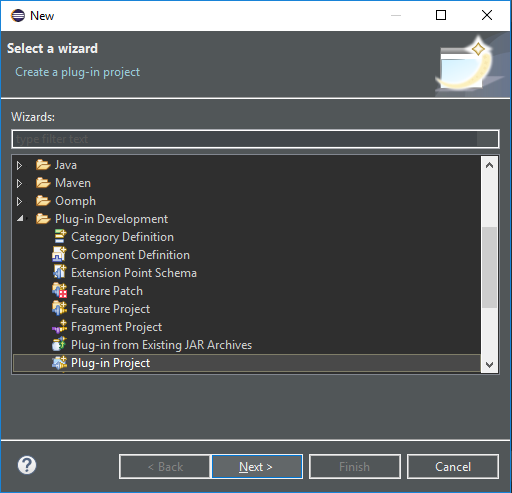
\includegraphics[height=5.5cm]{images/Tutorial4.png}} 
\\
  (a) & (b)
\end{tabular}
  \\[2pt]	
\begin{tabular}{@{}c@{\hspace{3mm}}c@{\hspace{3mm}}c@{}} 
  \fbox{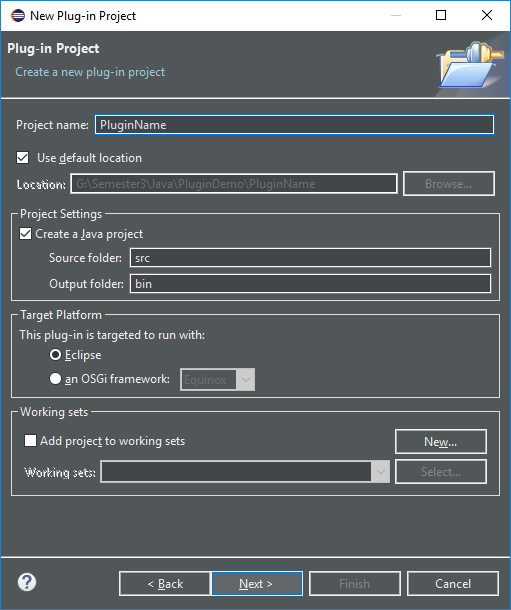
\includegraphics[height=5.5cm]{images/Tutorial5.png}} &
  \fbox{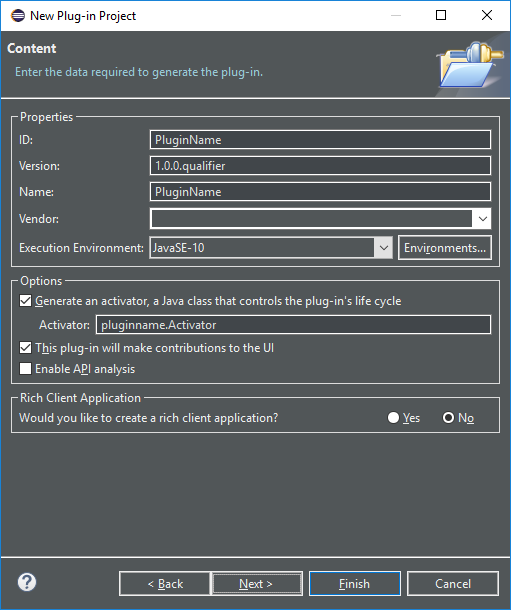
\includegraphics[height=5.5cm]{images/Tutorial6.png}} &
  \fbox{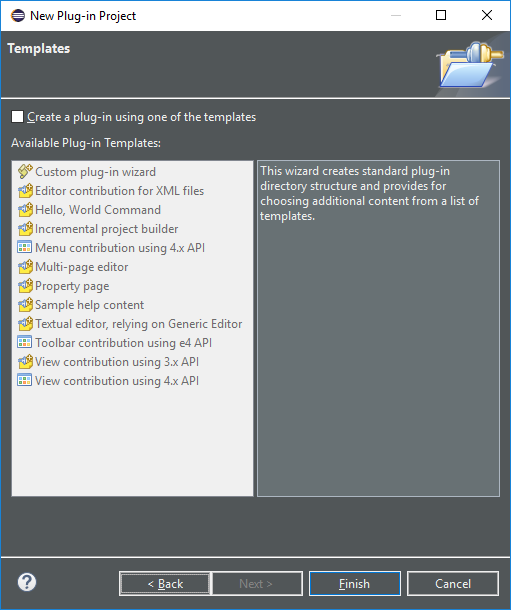
\includegraphics[height=5.5cm]{images/Tutorial7.png}} 
\\
  (c) & (d) & (e)
\end{tabular}
\caption{ Consecutive steps of plugin project creation. Launching creation wizard (a \& b), project options wizard (c), plugin options wizard (d) and template wizard (e). }
\label{fig:pluginWizard}
\end{figure}

Once the project is created it can be seen in \textit{Package Explorer}. It already contains \textit{build.properties} and \textit{MANIFEST.MF} files and \texttt{Activator} class. By clicking on the manifest file a special editor opens up on \textit{Overview} tab. Fig. \ref{fig:pluginProject} presents generated project structure and depicts manifest editor.

\begin{figure}[hbt!]
\centering\small
\begin{tabular}{@{}c@{\hspace{2mm}}c@{}} 
    \fbox{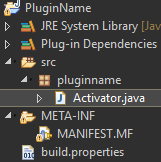
\includegraphics[height=4.5cm]{images/Tutorial8.png}}  &
  \fbox{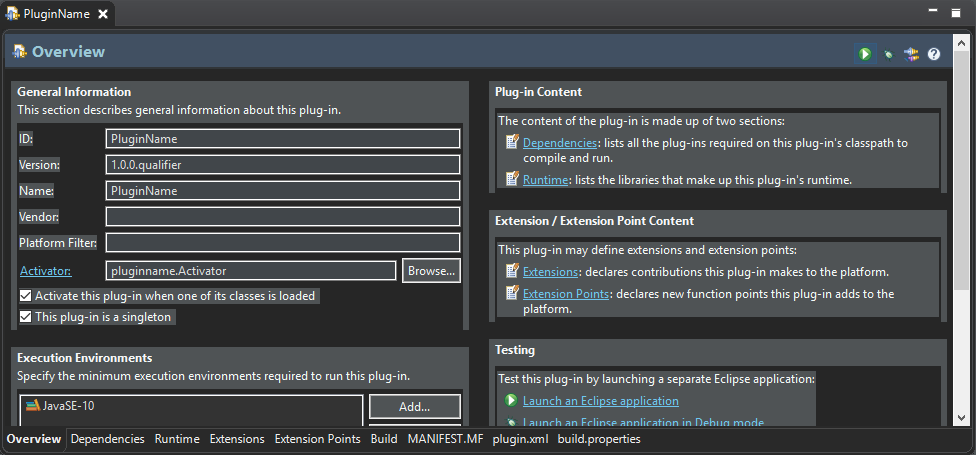
\includegraphics[height=4.5cm]{images/Tutorial9.png}} \\
  (a) & (b)
  \end{tabular}
\caption{ Project structure(a), manifest editor (b). }
\label{fig:pluginProject}
\end{figure}

\subsection{Adding extensions}

Adding a toolbar button requires extending the \textit{org.eclipse.ui.menus} extension point. This can be in the \textit{Extensions} tab, where by clicking the \textit{Add} button another wizard appears. This wizard allows us to browse, search and select necessary extension point. When extension point of interest is found and confirmed with \textit{Finish} button, the new extension point is visible as added into the list. By right-clicking the item a drop down menu is displayed, opening certain options for this item. To add a toolbar, a new menu contribution needs to be created first. Its \textit{locationURI} field must be set to \textit{toolbar:org.eclipse.ui.main.toolbar}. The location specifies where the extension will be placed. The contribution has to be extended by a toolbar with specified id. In order to provide a functionality to it, a command has to be created first. Analogically, at the beginning \textit{org.eclipse.ui.commands} extension point has to be added to the list, then extended by a new command, whose id and name should be specified. Each of the steps is presented in Fig. \ref{fig:menusExtension}.

\begin{figure}[hbt!]
\centering\small
\begin{tabular}{@{}c@{\hspace{3mm}}c@{\hspace{3mm}}c@{}} 
  \fbox{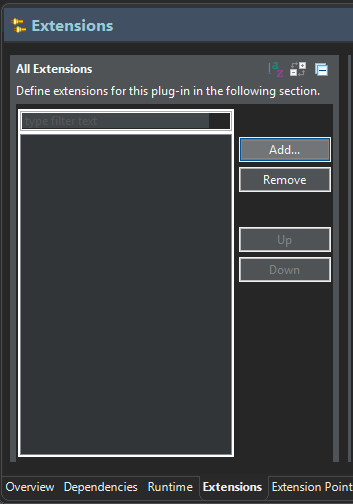
\includegraphics[height=4.8cm]{images/Tutorial10.png}} &
  \fbox{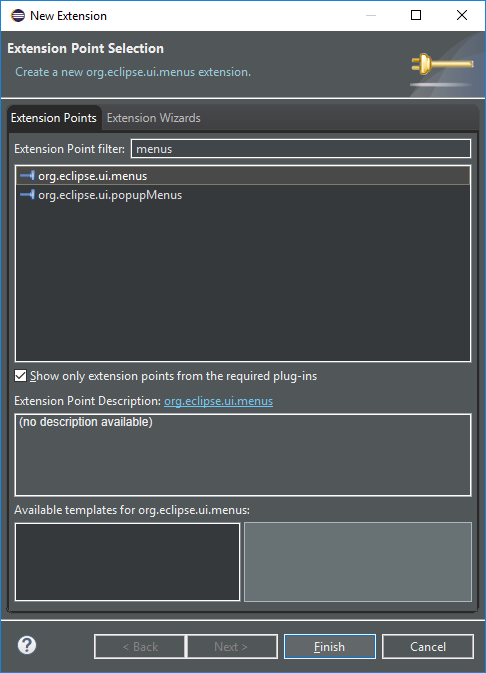
\includegraphics[height=4.8cm]{images/Tutorial11.png}} &
  \fbox{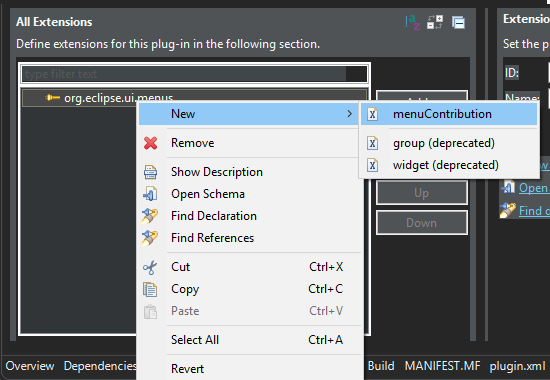
\includegraphics[height=4.8cm]{images/Tutorial12.png}} \\
  (a) & (b) & (c)
  \end{tabular}
  \\[2pt]
\begin{tabular}{@{}c@{\hspace{3mm}}c@{}} 
  \fbox{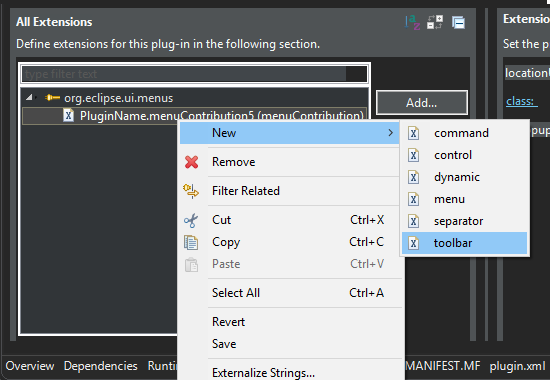
\includegraphics[height=4.8cm]{images/Tutorial13.png}} &
  \fbox{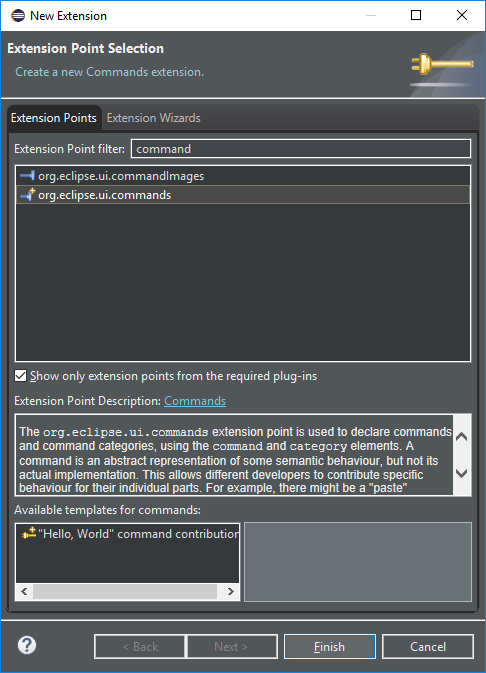
\includegraphics[height=4.8cm]{images/Tutorial14.png}} \\
  (d) & (e) 
  \end{tabular}
\caption{ Extenstion points list in Extenstions tab (a), addition of \textit{org.eclipse.ui.menus} (b), addition of menu contribution and a toolbar (c \& d), addition of \textit{org.eclise.ui.commands} (e).}
\label{fig:menusExtension}
\end{figure}


 When a command is triggered, its handler performs specified action. To assign a handler to the command, its name needs to be put into the \textit{defaultHandler} field (or selected via \textit{Browse} button to the right). In this case a new handler is to be implemented in a form of a new class that extends \texttt{AbstractHandler}. Resulting class presented in Program \ref{list:clickHandler} will only display a dialog with text. Now that the command is created it can be used in a toolbar button. Assigning the command to the toolbar is done in a similar manner as the rest of the extensions. It is important to give correct command's id in a field named \textit{commandId}. These steps are depicted in Fig. \ref{fig:toolbarCommand}.
 An image can be added to the button via \textit{icon} field, this time it is 16x16 pixels \textit{.png} file. If everything was done correctly, the program can be run as ``Eclipse Application''. The plugin's toolbar should be visible in a menu with the chosen image and once clicked, the dialog should appear as shown in Fig. \ref{fig:resultingPlugin}. That concludes the example. More detailed information can be found in the official documentation \cite{eclipse2019}.
 
 \begin{program}[hbt!]
    \caption{Start of interpretation procedure.}
    \label{list:clickHandler}
    \begin{JavaCode}
public class ToolbarClickHandler extends AbstractHandler {
	@Override
	public Object execute(ExecutionEvent event) throws ExecutionException {
		MessageDialog.openInformation(HandlerUtil.getActiveWorkbenchWindow(
                event).getShell(), "Info", "You clicked the button!");
		return null;
	}
}   \end{JavaCode}
\end{program}


\begin{figure}[hbt!]
\centering\small
\begin{tabular}{@{}c@{}} 
  \fbox{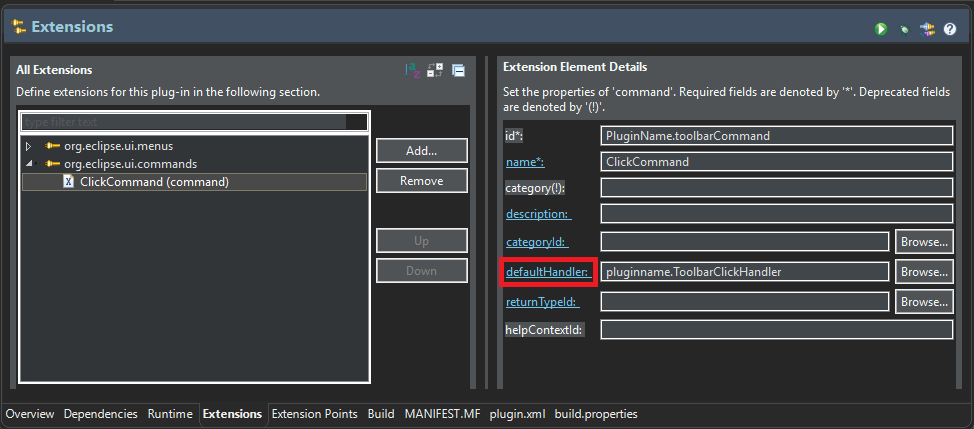
\includegraphics[height=5cm]{images/Tutorial15.png}} \\
  (a) 
  \end{tabular}
  \\[2pt]
\begin{tabular}{@{}c@{\hspace{2mm}}c@{}} 
  \fbox{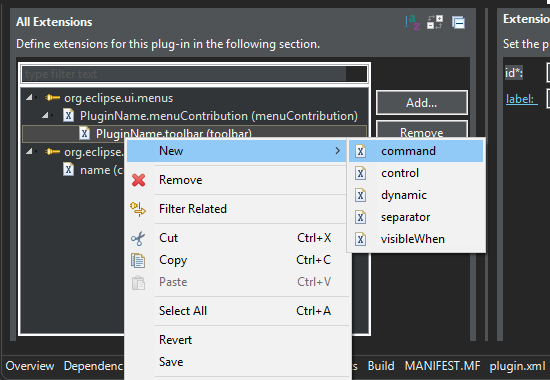
\includegraphics[height=4cm]{images/Tutorial16.png}} &
  \fbox{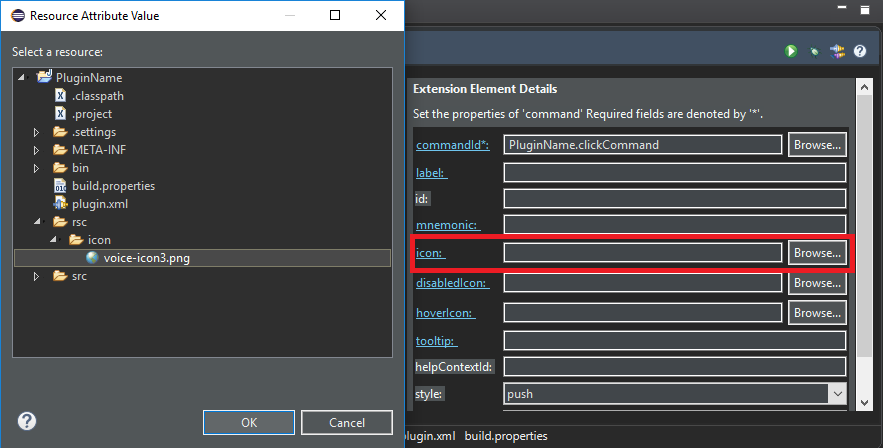
\includegraphics[height=4cm]{images/Tutorial17.png}} \\
  (b) & (c) 
  \end{tabular}
\caption{Field for command's default handler (a). Addition of command to the toolbar (b \& c). }
\label{fig:toolbarCommand}
\end{figure}


\begin{figure}[hbt!]
\centering\small
  \fbox{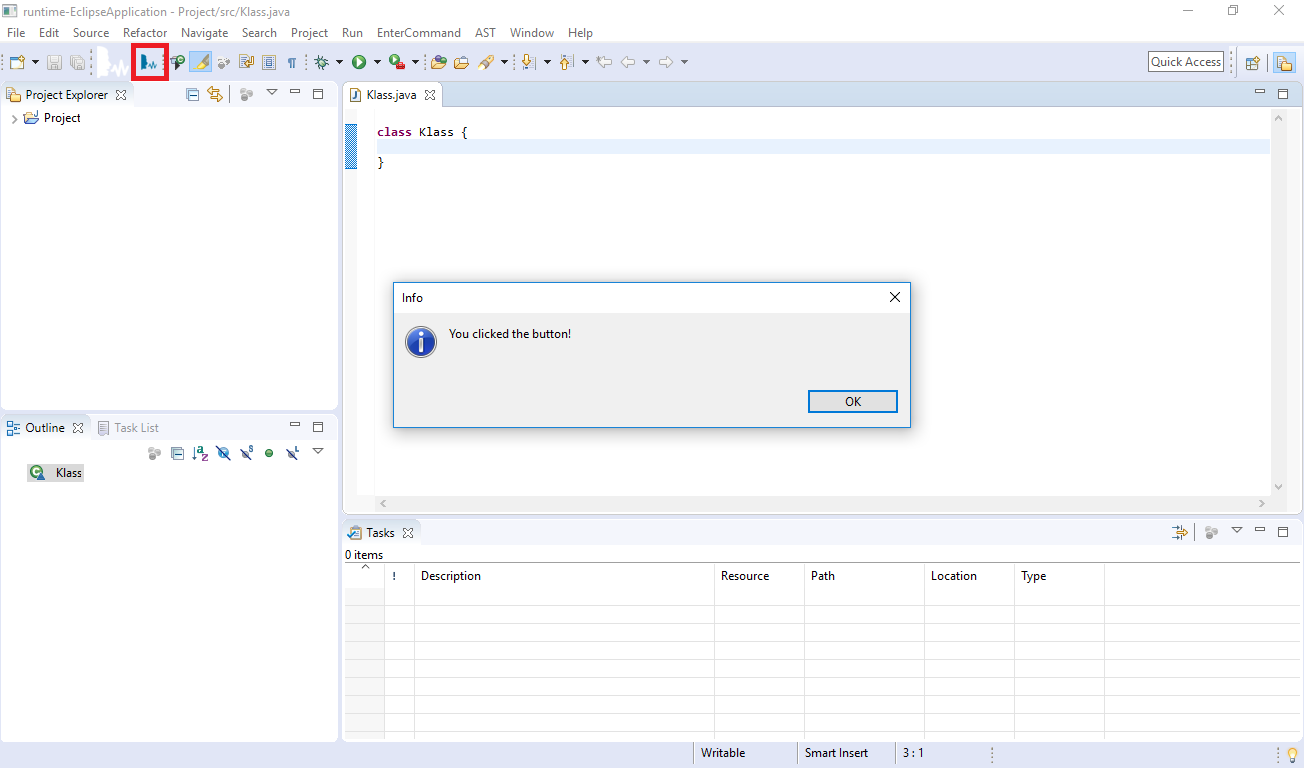
\includegraphics[width=0.9\textwidth]{images/Tutorial18.png}}
\caption{ Resulting plugin. }
\label{fig:resultingPlugin}
\end{figure}

\section{Speech Recognition tools}

Three different speech recognition tools are integrated into the project - two are different implementations of CMUSphinx toolkit, which is open-source and free of charge, and one is using Google Cloud Speech-to-Text API. Subsections below describe each of them in more detail. Before that, however, at the beginning a short introduction into how speech recognition works is given.

\subsection{Explaining speech recognition}

In a nutshell, humans communicate with each other using language. This languages consists of sentences, and these consists of words. Focusing only on the spoken aspect of a language, words are made out of subwords such as syllables, which in turn are made out of units of sound called phonemes. It is a simplification, however, as the sound of the phonemes can vary depending on the speed of speech, context, speaker, accent \etc In English language there are roughly 40 phonemes. It is these elements that the computer tries to match in order to recognize a word. 

At first, a couple of sentences on how voice is being transferred to the computer. Voice is a sound wave created by a vocal apparatus that produces vibrations in the air. A microphone converts the sound into electrical signal. This signal (as the sound itself) is continuous (analog). In order for a computer to understand this signal it has to be converted into a digital one. This is done by analog-to-digital converter (ADC), which performs certain operations such as sampling, filtering, normalization, adjusting to match the speed of a template \etc Once the signal is ready, it is then divided into small portions (frames) of a few hundredths or thousandths of seconds which are a subset of phonemes called senones. These segments are used to match known phonemes.

The rest of the process is belongs to Machine Learning domain. For each frame a number of features are extracted. Each feature is a characteristic aspect of the segment which together with others creates a feature vector - a fingerprint of a kind. These features are used to match a model using complex mathematical functions and probability to determine the most likely outcome. Because of computational limitations and complexity of feature matching, the number of features should be as small as possible, yet the features should be strong enough to enable distinction between the segments. \\
In speech recognition the most commonly used model is called Hidden Markov Model (HMM). During the process of matching each phoneme is assigned a specific probability score based on previously done training and a dictionary. The process does not consider one phoneme at a time, but it also takes into account neighbouring phonemes, therefore it is contextual. It is done on the level of building words, but also the whole phrases.

There are two models that are necessary for speech recognition: acoustic and language model. The former contains acoustic properties for each senone. This model can be context-dependent or context-independent. The latter is used to restrict the search for words by defining which word could follow the one preceding it. In result this significantly quickens the process by focusing on the most probable words. Otherwise, having a vocabulary of 60.000 words and a sequence of three words the program would need to check 216 trillion possibilities. \\ A component that is required to combine these two models provides some sort of a mapping between the phonemes and words. This can either be done by so called phonetic dictionary, which is a list of words with phonemes representing them, or by more efficient complex mathematical function achieved by machine learning algorithm.

\subsection{CMUSphinx}

The initial idea was to base the whole project on available free of charge software elements. An open-source Speech Recognition engine was therefore preferable. After a small research CMUSphinx was selected as it was recommended most often. It was said that it is accurate enough, easy to implement and with very broad documentation. Its documentation is indeed quite well described and is very helpful \cite{CMUSphinx}. It is stated there that CMUSphinx is \textit{leading speech recognition toolkit with various tools used to build speech applications}. On top of that \textit{CMUSphinx contains a number of packages for different tasks and applications}. The toolkit provides different tools, including two recognizer libraries: Pocketsphinx and Sphinx4. Pocketsphinx is a lightweight library written in C, recommended when speed and portability are the main factors or when recognition is to be run on embedded device. Sphinx4 on the other hand is easily adjustable, modifiable recognizer written in Java. It is said that its flexibility makes it possible to quickly build a system. When it comes to selection between the two, it is not accuracy that should be the main criteria but rather the nature of application. In this project Sphinx4 was the first choice mainly for the sole reason, that it is a pure Java library and it is simple to integrate it to Java project, which CodeSpeech is. After further reading, however, the author of this thesis decided to also give Pocketsphinx a try. That is because of the additional recognition method that Pocketsphinx provides which Sphinx4 does not, namely keyphrase recognition. Other two methods that are available for both technologies are continuous speech and grammar based recognition. All three of the previously mentioned methods of recognition will be explained later.


\subsubsection{Sphinx4}

As stated in the documentation, integration of Sphinx4 was relatively easy and quick. The only thing that was needed to use its API were two Java library files, namely sphinx4-data.jar and sphinx4-core.jar. The former consists of acoustic model, dictionary and language model, the latter is API itself. After giving it a try it turned out that recognition of continuous speech did not work well for the author of the thesis. The accuracy, even though not measured, was clearly poor. 

\subsubsection{PocketSphinx}

Integrating PocketSphinx into the project was a completely different story. It lasted for plenty of hours that were spent on solving  continuously coming up issues occurring on different stages. Problems followed the whole process: from correctly building libraries from the source, through usage of Swig to build JNI Java files from C code (although bless the creators of CMUSphinx that this possibility is present and the whole library does not have to be translated to JNI manually) to finally use the generated JNI files as a library in a project. Error messages were often misleading and resulted in additional hours spent on looking for a mistake (which are very easy to make). To be fair, PocketSphinx was never intended to be used in Java projects (that is what Sphinx4 is for), and yet a possibility exists.

When finally all of the necessary libraries were built and loaded, the implementation could be continued. At first an Android project using PocketSphinx available online was used as a template. The accuracy of PocketSphinx was similarly poor to Sphinx4's, nevertheless the results were being returned faster. 

With both technologies giving not satisfying enough results, the author decided to try to adapt models used by CMUSphinx in order to improve the accuracy of the recognition. 

\subsubsection{Model adaptation}

In cases of low accuracy the documentation of CMUSphinx proposes to adapt acoustic model. This can be done relatively easily using Sphinxbase library which \textit{provides common functionality across all CMUSphinx projects}. Sphinxbase is provided together with PocketSphinx package. Adaptation was performed based on corresponding chapter of the documentation. Accordingly, twenty audio transcriptions consisting of the author reading multiple words were recorded, proper text files were created and finally the model was adopted. It did not bring the results that were hoped for, unfortunately, accuracy remained poor. It is possible, that for a significant improvement even more recordings (at least hundred) are necessary, because of time limitation however, this process was skipped. 

Since the adaptation of the acoustic model did not end in significant increase of accuracy of recognition, another means of improvement mentioned in the documentation were performed. These included building a new language model, new dictionary and combination of all three steps. These tasks were quite difficult to do on Windows OS and turned out to be easier on Linux. In the end no success was achieved.

The creators of CMUSphinx explained that the low accuracy might be related to the author's accent. The models were built for American speakers and thus does not work well for people talking differently. Even British people won't be able to achieve high accuracy unless they build a new model their own voices. Building the new model from scratch requires a lot of time, plenty of hours of recordings and is a very complicated process. Due to the limited amount of time it was decided to move on and find another speech recognition tool. 

\subsection{Google Cloud Speech-to-Text}

Google Cloud Speech-to-Text is a service that enables developers to convert audio to text by applying powerful neural network models hosted in a cloud. It recognizes 120 languages and variants, and has an API that is easy to use. On the official website of the service it is possible to try it out before making a decision, and without a doubt this recognition is far better than the one provided by CMUSphinx. API was indeed very simple to integrate to Java project and worked almost out of the bat. This service is not free of charge however. The pricing as it was at the time of writing this thesis is presented in Fig. \ref{fig:cloudSpeechPricing}. As can be seen, there exists a free tier up to 60 minutes of recording that lasts for a year. This is very fortunate, because the initial assumption was to create programming by voice prototype without any money spend. The free tier allows the author to create the prototype and see if the idea of programming by voice in a plugin is possible at all. Once the hypothesis is confirmed, more time can be put into either enhancing current CMUSphinx models, creating a completely new one or applying yet another free-of-charge tool with good enough accuracy.

\begin{figure}[hbt!]
    \centering
    \fbox{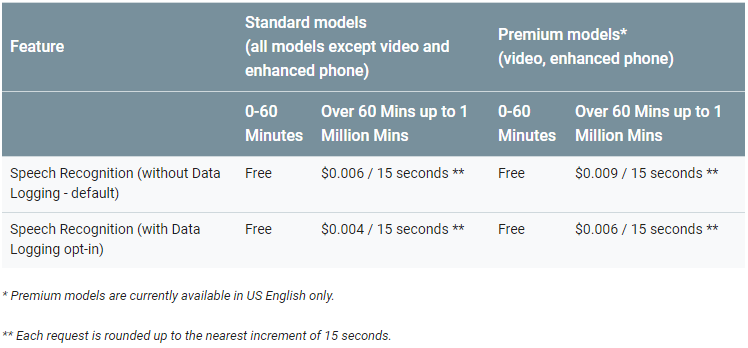
\includegraphics[width=0.85\textwidth]{images/CloudSpeechPricing.png}}
    \caption{Pricing of Google Cloud Speech-to-Text service (taken from official website \cite{CloudSpeech2019}).}
    \label{fig:cloudSpeechPricing}
\end{figure}

Google Speech-to-Text being a cloud service, obviously requires Internet access. The recording of voice is done on the local machine, but once an utterance is finished, it is being sent over to Google server and there neural network models perform recognition. After it is done the result is sent back via callback. That is another difference with previously mentioned technologies, which run entirely on local machine and do not require an Internet connection.

\subsection{Comparison of SR tools}

A summary of certain features belonging to aforementioned tools is presented in the Tab. \ref{tab:comparisonSR}. This table might help in making a decision as to which technology should be used in the development of future Java projects. The difficulty of integration is of course relative, however, the fact that Sphinx4 and Google Cloud Speech-to-Text tools already have existing, ready to use APIs written in Java while PocketSphinx does not, plays a big part here. PocketSphinx library has to be built, then JNI code generated \etc The time needed for for all theses steps might differ depending on the programmers skills and knowledge, nevertheless the number of steps required for integration is significantly higher in comparison to the other two. It is of course understandable as PocketSphinx was never intended to be used for Java projects. \\
In addition, all engines were tested in terms of recognition time and Word Error Rate (WER) metric. The formula for WER is 
 $$   WER = \frac{I + D + S}{N}, $$
where I is the number of inserted words, D is the number of deleted words, S is the number of substituted words and N is the number of words in the original (reference) sentence. In controversial situations like e.g. when one word from the reference text was recognized as n words, one substitution and n - 1 insertions were counted. In a reverse situation, when multiple words were recognized as one, the entry had one substitution and n - 1 deletions. In order for the comparison to be more accurate, test was performed on recordings rather than live speech. The reason for that is to ensure that exactly the same audio is analysed by each software. For this purpose ten sentences were recorded and used by each tool's file analyser. Resulting sentences were written to the file and then WER was manually calculated. 

\begin{table}[hbt!]
    \caption{Comparison of used SR technologies in regard of features important for Java developers.}
    \label{tab:comparisonSR}
    \centering
    \setlength{\textwidth}{5mm} % separator between columns
    \def\arraystretch{1.25} % vertical stretch factor
    \begin{tabular}{|r||c|c|c|}
        \hline
        & \emph{Sphinx4} & \emph{PocketSphinx} & \emph{Google Speech-to-Text} \\
        \hline
        \hline
        Integration difficulty & Easy & Difficult & Easy \\
        \hline
        Price & Free & Free & Free-tier, paid \\
        \hline
        Internet connection & No & No & Required \\
        \hline
        WER [\%] &  88,2 & 94,3 & 17  \\
        \hline
        Average time [s] &  19,76 & 2,12 & 2,17 \\
        \hline
    \end{tabular}
\end{table}

The results of this test show that when it comes to performance Google Cloud Speech-to-Text is clearly the winner. Not only it does the recognition quickly despite the need of sending and receiving data through the Internet, but also has the smallest WER score of 17\%. PocketSphinx recognizes in a similar speed (in this experiment slightly faster), but its WER is very high (around 95\%). Sphinx4 did a bit better than PocketSphinx in terms of recognition, but was incredibly slow (almost 10 times slower than the other two). Taking all that into consideration, Google Cloud Speech-to-Text was used as a main speech recognition engine, although all three were integrated into the system. Perhaps in the future CMUSphinx models will be trained to increase the performance.

\section{ANTLR}

The end goal of the finished programming by voice product is to perform operations using natural sentences. At the end of the previous chapter an issue related to the way code is read by different people is discussed. The same problem might appear when it comes to steering the program by voice through the use of different commands. Taking that into consideration, it was decided that for the control over the program by voice commands an interpretation of specified grammar will be used. Although grammars are usually quite strict when it comes to token recognition because each of the required elements must occur in a right position, they also allow a certain amount of flexibility by enabling representation of tokens by different keywords/phrases. Once decided upon this approach, a proper tool had to be selected for parsing and managing grammars and finally the choice was ANTLR (ANother Tool for Language Recognition). ANTLR as described on the official website 
\begin{quote}
    \begin{english}
   is a powerful parser generator for reading, processing, executing, or translating structured text or binary files. It's widely used to build languages, tools, and frameworks. From a grammar, ANTLR generates a parser that can build and walk parse trees \cite{ANTLR2019}.
    \end{english}
 \end{quote}
ANTLR turned out to be exactly what was needed, giving a lot of options in the way the sentence is parsed. This flexibility is a great advantage of ANTLR. Below more information about working with ANTLR are given.

\subsection{Typical workflow}

At first ANTLR tools have to be installed and then grammar file with \textit{.g4} extension created. Then, running ANTLR tools against the grammar generates code that enables handling each specific token or keyword at any time. Whenever the change in grammar is made, new files have to be generated and applied to the project. The most important from the point of view of developer are listeners or visitors files (depending on the option). They provide methods that are triggered whenever a token is entered or exited. Many custom listeners or visitors can be implemented, each allowing for alternative interpretation of the same token depending on a current state of the program. The whole process was divided into three parts: installation of ANTLR tools, writing a grammar and generation of the files.

\subsubsection{ANTLR tools}

ANTLR consists of two parts: the tool used to generate lexer and parser, and the runtime needed to run them by the end software. The tool is the Java program and it requires at least Java 1.7 installed on a working machine. To install the program it needs to be downloaded from the official website from a download section and then added to the classpath of the system. When done, \texttt{antlr4 <options> <grammar-file-g4>} command can be used in order to generate files needed by the end software. Options allow generation thereof to a specific language other than Java (which is set as default) \eg Python or JavaScript, or to choose between generation of listeners (default) or visitors. \\
This is one way of using ANTLR. During this project yet another approach was used. Generation of needed files based on the grammar was done through another external ANTLR project. It is a simple Java project which uses ANTLR libraries via Maven. The grammar is placed in project's \textit{src/main/antlr4} folder. Generation is then done using \texttt{mvn package} command. 

The end Java program that will use ANTLR can be set up either by Gradle, Maven or manually. Because of the conflict that occurs between Eclipse plugin project and other manifest-based ones, for now the CodeSpeech is set up manually. Addition of external libraries such as antlr4-runtime.jar to Eclipse plugin project can be done via \textit{Runtime} tab of the manifest editor in the \textit{Classpath} area as shown in Fig. \ref{fig:jarAddition}.

\begin{figure}[hbt!]
    \centering
    \fbox{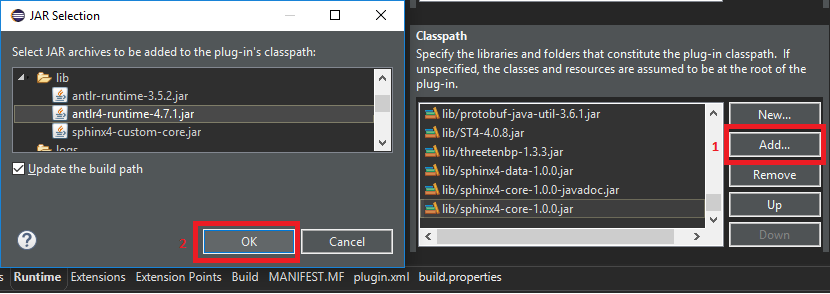
\includegraphics[width=\textwidth]{images/ANTLR1.png}}
    \caption{Addition of external library. }
    \label{fig:jarAddition}
\end{figure}

\subsubsection{Grammar}

Grammar consists of lexer and parser rules. Lexer, also known as tokenizer analyzes text and assigns a proper token to parts of it. Parser takes these tokens and organizes them into abstract syntax tree. Both parser and lexer perform their tasks using so called rules. In ANTLR lexer and parser rules are distinguished by the first character of the rule's name: parser rules start with lower case and lexer rules with upper case. For better readability it is common to write the name of the lexer rules completely in upper case. Lexer rules are usually put at the bottom of the grammar, however, from the ANTLR's point of view it does not matter, it is just a standard of organization. It is possible to divide parser and lexer rules to two separate files. In Program \ref{list:grammar} both types of rules are in one file, with lexer rules being at the bottom. 

\begin{program} [hbt!]
    \caption{Example of grammar file's content. This grammar allows creation of simple mathematical equations. }
    \label{list:grammar}
    \begin{JavaCode}
grammar BasicMath;		

/*
 * Parser Rules
 */
program:	(equation NEWLINE)* ;
equation:	equation ('*'|'/') equation
    |	equation ('+'|'-') equation
    |	INT
    |	'(' equation ')'
    ;

/*
 * Lexer Rules
 */
fragment DIGIT : [0-9] ;
INT     : DIGIT+ ; 
NEWLINE : [\r\n]+ ;
WHITESPACE : (' ' | '\t') ;    \end{JavaCode}
\end{program}

As it can be seen, the content of a rule is placed between a colon and a semi-colon defined after the name. A \texttt{fragment} rule allows to create reusable blocks for lexer rules. Parser rule can consist of parser and lexer rules. It can also be seen that ANTLR allows recursion, so referencing itself in the rule. A few symbols that exist in this example are: ``|'' for an alternative, ``+'' for one or more occurrence, ``*'' for zero or more, parentheses for definition of a subrule. Characters, whole words or phrases that are to be recognized are defined in single quotes. More examples, symbols and other interesting information can be found in the official documentation \cite{ANTLRDOC2019}.

\subsubsection{Generation}

Once the grammar is finished a time has come for generation. Without regard for the method of performing that procedure (two were mentioned before), the generated files have to be moved to the project source folder in order to be used. Every time the grammar is modified, the process has to be repeated to apply the changes. This occurs quite often during the development and might be bothersome, however, a simple shell script can help in automation of the whole procedure, which in the end can save a lot of time. The script at first initializes generation by running \texttt{mvn package} in the home folder of ANTLR project. Then it adds proper package name via combination of \texttt{echo}, \texttt{cat} and \texttt{mv} commands and later moves them, to the target directory via \texttt{mv}. This solution speeds up the process, leaving refreshing the project as the only thing to do. 

The generated files are named according to the grammar's file name. If the grammar is named \textit{BasicMath}, then the resulting files will be \textit{BasicMathLexer.java}, \textit{BasicMathParser.java}, \textit{BasicMathListener.java} and \textit{BasicMathBaseListener.java}. File extension of course depends on the selected target programming language. In case of choosing visitors to be created those would replace listener files. In addition, \textit{.interp} and \textit{.tokens} files appear, but those are not needed by the runtime. Program \ref{list:listener} presents an interface contained in \textit{BasicMathListener.java} file. Its implementation in form of abstract class is consisted in \textit{BasicMathBaseListener.java}.

\begin{program} [hbt!]
    \caption{A generated listener. }
    \label{list:listener}
    \begin{JavaCode}
// Generated from BasicMath.g4 by ANTLR 4.7.1
import org.antlr.v4.runtime.tree.ParseTreeListener;

/**
 * This interface defines a complete listener for a parse tree produced by
 * {@link BasicMathParser}.
 */
public interface BasicMathListener extends ParseTreeListener {
	/**
	 * Enter a parse tree produced by {@link BasicMathParser#program}.
	 * @param ctx the parse tree
	 */
	void enterProgram(BasicMathParser.ProgramContext ctx);
	/**
	 * Exit a parse tree produced by {@link BasicMathParser#program}.
	 * @param ctx the parse tree
	 */
	void exitProgram(BasicMathParser.ProgramContext ctx);
	/**
	 * Enter a parse tree produced by {@link BasicMathParser#equation}.
	 * @param ctx the parse tree
	 */
	void enterEquation(BasicMathParser.EquationContext ctx);
	/**
	 * Exit a parse tree produced by {@link BasicMathParser#equation}.
	 * @param ctx the parse tree
	 */
	void exitEquation(BasicMathParser.EquationContext ctx);
}    \end{JavaCode}
\end{program}

As it can be seen, for each parser rule there exist two methods: for entering and exiting specified parser rule. This allows the end program for performing specific actions depending on the implementation. Because many custom listeners can be created and changed back and forth during runtime, a different operation can be performed on the same keyword depending on the context. This elasticity of ANTLR, as well as ease of use, well written and broad documentation and active support were the main factors that decided upon selecting ANTLR as an interpretation tool. 

\subsection{ANLTR plugin}

To make the work with ANTLR easier, it can also be integrated into many IDEs. There exists a plugin for Eclipse called \textit{AntlrDT Tools Suite for Eclipse}, which provides following features:

\begin{itemize}
   \item Advanced Syntax Highlighting
   \item Automatic Code Generation (on save)
   \item Manual Code Generation (through External Tools menu)
   \item Code Formatter (Ctrl+Shift+F)
   \item Syntax Diagrams
   \item Advanced Rule Navigation between files (F3 or Ctrl+Click over a rule)
   \item Quick fixes
\end{itemize}

Syntax diagram is a very helpful feature which helps to visualise how the grammar is constructed. An example can be seen in Fig. \ref{fig:grammarSyntaxDiagram}.

\begin{figure}[hbt!]
    \centering
    \fbox{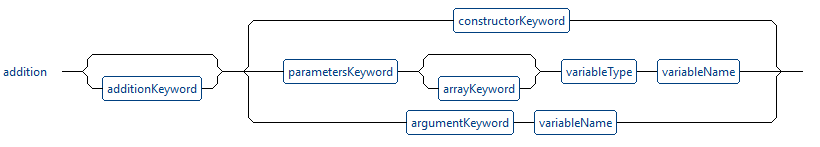
\includegraphics[width=\textwidth]{images/GrammarSyntaxDiagram.PNG}}
    \caption{An example of syntax diagram.}
    \label{fig:grammarSyntaxDiagram}
\end{figure}

\chapter{Method}
\label{cha:Method}

 %- requirements, design, user study (if done)
 %- automating implementation?

This chapter goes through requirements definition and design stages. It is here, where one can find specification of the functional and non-functional requirements, use cases and a plan of general architecture of the system. 

\section{Requirements}

This section is devoted to stating requirements. Functional and non-functional requirements have been divided into two subsections. At the end a couple of constraints that the project has are mentioned.

\subsection{Functional requirements}
Functional requirements should define what the system ought to do. Below the main requirements are presented in the form of a list. 

The product shall:
\begin{itemize}
  \item properly recognize speech,
  \item create source code,
  \item modify source code,
  \item run a program,
  \item debug a program,
  \item allow navigation in the file,
  \item allow navigation in the workspace.
\end{itemize}

The system's main functionality can be stated as ``translating user's speech into an operation that is to be performed inside IDE''. Each particular requirement corresponds to one type of operation. In other words, the system should respond to user's input, which is always audio data. The resulting output is an action performed by the system. When the user wants, for example, to create a for loop, he/she has to speak out a proper sentence which the system should interpret. 

Because CodeSpeech is to allow writing programs by voice, of course it needs to be able to perform every task that is required in programming. It needs to provide a way to create source code, modify thereof, navigate inside files as well as in between files. Running and debugging the program are also inherent parts of programming, therefore should also be possible.

These requirements are a certain simplification, as \eg the term ``create source code'' could mean creation of variables, methods or other structures, similarly ``modify source code'' could mean deletion of a line, changing the name of the structure, adding a parameter \etc. Each of the requirements consists of many elements that could be stated on its own. For simplicity a generalization was made.

\subsection{Non-functional requirements}
Non-functional requirements describe what the system ought to be like. Below there is a list of the main characteristics that define a good implementation of the system.

The product shall:
\begin{itemize}
  \item be easy to use - to ensure high usability,
  \item interpret user’s natural English sentences - the system is directed towards English speakers,
  \item work with non-native speakers - there are many different accents and the system should work with most of them,
  \item be reliable - system should not crash or lose data,
  \item not perform many mistakes - to ensure usability and decrease frustration,
  \item have a way to correct mistakes - mistakes done either by the system or the user should have an easy way of being corrected,
  \item be intuitive - should require little time to be learned,
  \item inform about errors and a way to prevent them - user has to be always informed of what is happening,
  \item quickly respond to the user - to increase productivity,
  \item give precise feedback - user should be able to understand what has happened, might have an influence on speech recognition,
  \item must work with Eclipse IDE - system is intended to work as an Eclipse plugin,
  \item be easily available from within Eclipse Market - acquiring and installation of the system should be easy and almost automatic, 
  \item run on Windows OS,
  \item run on Linux OS.
\end{itemize}

\subsection{Constraints}
CodeSpeech has couple of constraints resulting from either its nature or technology used. The first obvious constraint is a need of a microphone. The program is heavily dependent on audio input cannot be used without a way to record voice. Another constraint related to that is a requirement of usage in a quiet environment. In order to increase performance of recognition ambient noise should be decreased to the minimum. One software constraint is Eclipse IDE with JDT (Java development Tools) installed on the workstation as the system is intended to be a plugin. Finally, because of the use of selected speech recognition tool, CodeSpeech requires an Internet connection.

\section{Use cases}

Below one can find enlisted use cases with short description. They depict different actions that can be performed from the user's point of view, such as the creation of the specific code structure, moving the cursor to a given line \etc In Fig. \ref{fig:useCases} a visualization in the form of UML Use Case diagram is presented. The main use cases are:

\begin{enumerate}
  \item Creating source code - most important part of programming. It involves: \eg
    \begin{itemize}
     \item creation of project elements, such as project, package, compilation unit,
     \item creation of programming structures, such as variables, methods definitions, invocations, loops, if conditions \etc
   \end{itemize}
  \item Modifying source code - due to mistakes or constant development process, modification of source code is inevitable. Examples of modification: 
    \begin{itemize}
     \item name, type changes,
     \item values assignment, initialization,
     \item addition, removal of method parameters/arguments,
     \item deletion of a structure.
   \end{itemize}
   
  \item Local navigation (in file) - placing a cursor in a specific position in a file:
  \begin{itemize}
     \item vertical navigation (between lines),
     \item optional: horizontal navigation (by character/nodes \eg parameter).
   \end{itemize}
   
  \item Global navigation (between files) - such as:
  \begin{itemize}
     \item selection of other projects in the workspace,
     \item opening another compilation unit for modifications.
   \end{itemize}
   
  \item Calling Eclipse commands - programming is not only writing source code, it also involves other actions, which nowadays are built-in into IDEs. That is why CodeSpeech was selected to be an extension of such an environment and provide a way to \eg:
    \begin{itemize}
     \item put/enable/disable a breakpoint into a specific line,
     \item compile program,
     \item run/debug program.
   \end{itemize}
\end{enumerate}

\begin{figure}[hbt!]
    \centering
    \fbox{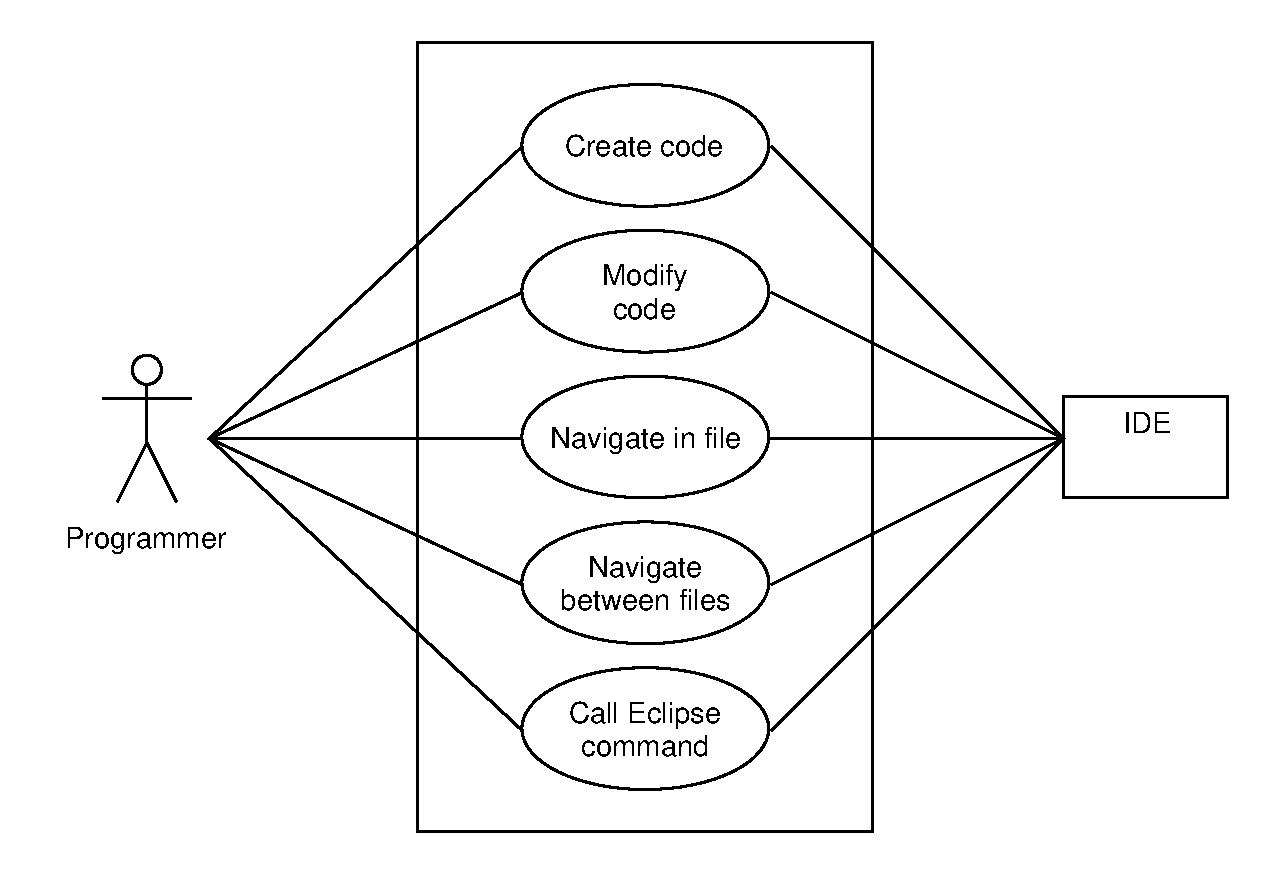
\includegraphics[width=\textwidth]{images/UseCaseDiagram.pdf}}
    \caption{Use Case diagram.}
    \label{fig:useCases}
\end{figure}
 
\leavevmode \\
\noindent
\textbf{Use Case 1}\\
User/actor name: Programmer\\
Description: Create code\\
Use Case Scenario:
\begin{enumerate}
  \item User speaks
  \item SR engine processes the audio signal and returns recognized speech in text 
  \item Plugin recognizes command
  \item Plugin performs operations on AST to create new code
  \item Plugin updates IDE
\end{enumerate}

\leavevmode \\
\noindent
\textbf{Use Case 2}\\
User/actor name: Programmer\\
Description:  Modify code \\
Use Case Scenario:
\begin{enumerate}
  \item User speaks
  \item SR engine processes the audio signal and returns recognized speech in text 
  \item Plugin recognizes command
  \item Plugin performs operations on AST to manipulate existing code
  \item Plugin updates IDE
\end{enumerate}

\leavevmode \\
\noindent
\textbf{Use Case 3}\\
User/actor name: Programmer\\
Description: Navigate in file\\
Use Case Scenario:
\begin{enumerate}
  \item User speaks
  \item SR engine processes the audio signal and returns recognized speech in text 
  \item Plugin recognizes command
  \item Plugin moves cursor to given position
\end{enumerate}

\leavevmode \\
\noindent
\textbf{Use Case 4}\\
User/actor name: Programmer\\
Description: Navigate between files\\
Use Case Scenario:
\begin{enumerate}
  \item User speaks
  \item SR engine processes the audio signal and returns recognized speech in text 
  \item Plugin recognizes command
  \item Plugin opens new editor and displays file's content
\end{enumerate}

\leavevmode \\ \\
\noindent
\textbf{Use Case 5}\\
User/actor name: Programmer\\
Description: Call IDE command\\
Use Case Scenario:
\begin{enumerate}
  \item User speaks
  \item SR engine processes the audio signal and returns recognized speech in text 
  \item Plugin recognizes command
  \item Plugin performs calls IDE's command
\end{enumerate}

\leavevmode

As it can be seen, the only thing required by the user to do is to speak the right command. The system then takes care of analyzing the speech and performing the right action.

\section{Design}
This section presents some ideas for the architecture of the system and its interface, discusses design choices backing them up with arguments, examples and summarises the advantages and disadvantages of these choices.

\subsection{System Architecture}
The structure of the system will consist of three main parts. One will be responsible for speech recognition, second for plugin management and the third for utterance interpretation. These are planned to be implemented in three structures: SpeechRecognizer, PluginManager and Interpreter, respectively. Fig. \ref{fig:architectureConcept} presents these components in simple UML diagrams.

\begin{figure}[hbt!]
\centering\small
\begin{tabular}{@{}c@{}} 
  \fbox{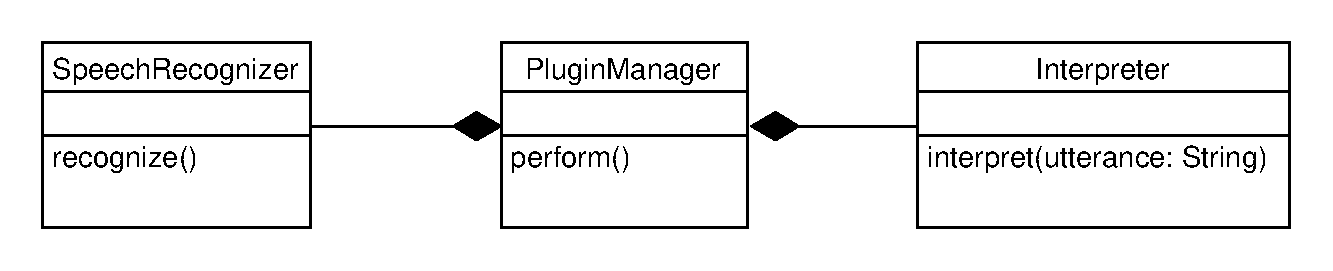
\includegraphics[width=\textwidth]{images/SimpleClassDiagram.pdf}} \\
  (a)  
  \\[10pt]
  \fbox{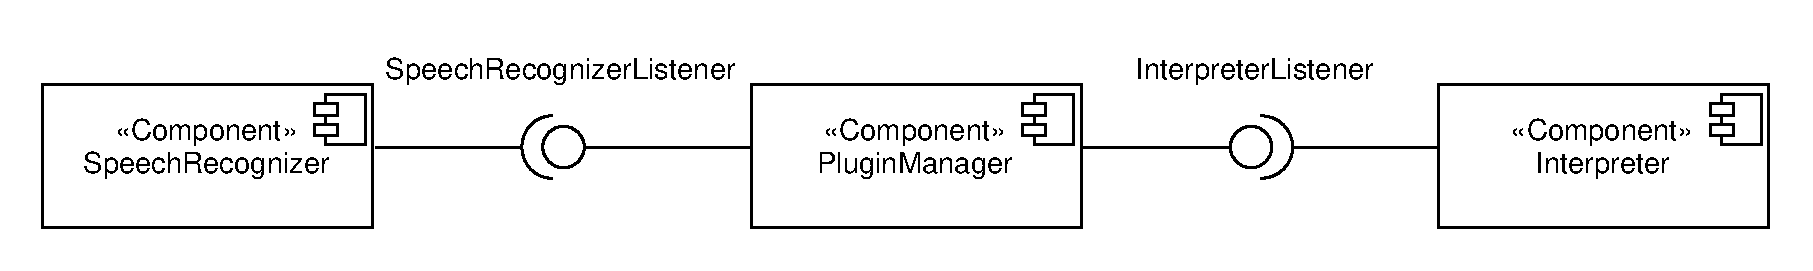
\includegraphics[width=\textwidth]{images/ComponentDiagram.pdf}} \\
  (b) 
  \end{tabular}
\caption{ Initial class diagram (a). Component diagram (b). }
\label{fig:architectureConcept}
\end{figure}

The main idea is like this: PluginManager is the main structure of the plugin so it initializes other structures and all necessary tools. This is due to the way Eclipse plugin structure look like. When plugin is on, SpeechRecognizer waits for audio input. When the user stops speaking, audio is treated by the implementation of currently used SR toolkit. When done, PluginManager is notified and receives the recognized utterance in the form of text. PluginManager then delegates the utterance to the Interpreter. Interpreter analyses the text and builds a proper Command object. Once the whole utterance has been walked through, the PluginManager is notified and receives the Command. Then, if everything is set, PluginManager executes the command and performs the action on IDE. The program can be interrupted and turned off at any stage of the recognition. Basic state diagram presenting the workflow is depicted in Fig. \ref{fig:stateDiagram}.

\begin{figure}[hbt!]
\centering\small
\begin{tabular}{@{}c@{}} 
  \fbox{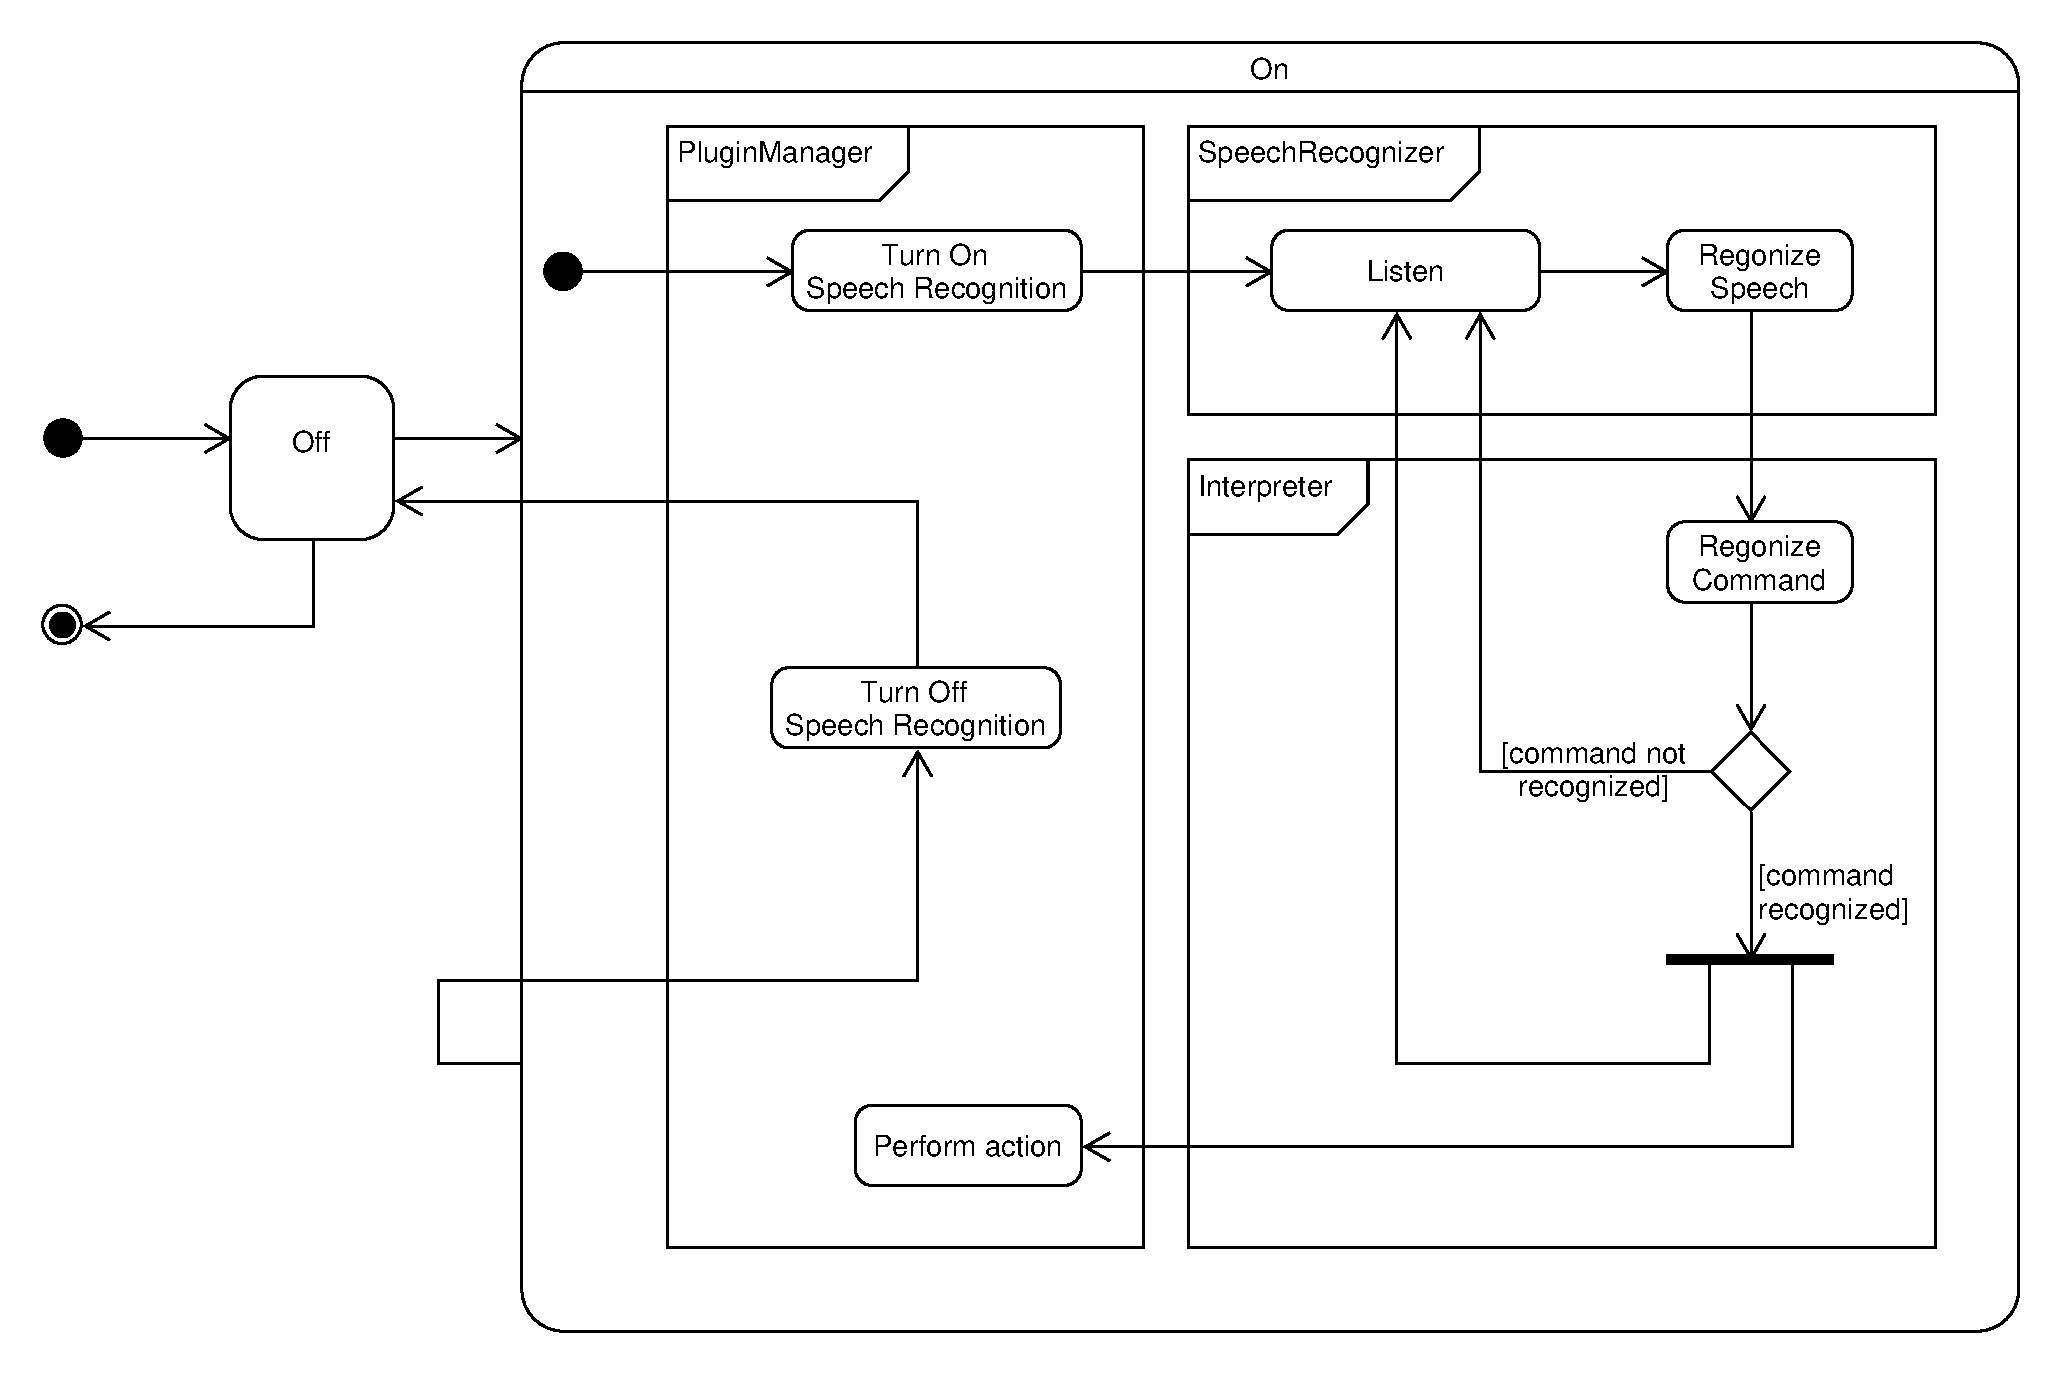
\includegraphics[width=\textwidth]{images/StateDiagram.pdf}}
  \end{tabular}
\caption{ State diagram of the program. }
\label{fig:stateDiagram}
\end{figure}

The system diagram is presented in Fig \ref{fig:systemDiagram}. Microphone does not have to be external, it can be one built into the laptop. Internet connection might be optional, depending on the system recognition tool that is being used. There might be a case in which a cloud service is utilized, and Internet connection is required. The system could be any which can run Eclipse IDE.

\begin{figure}[hbt!]
\centering\small
  \fbox{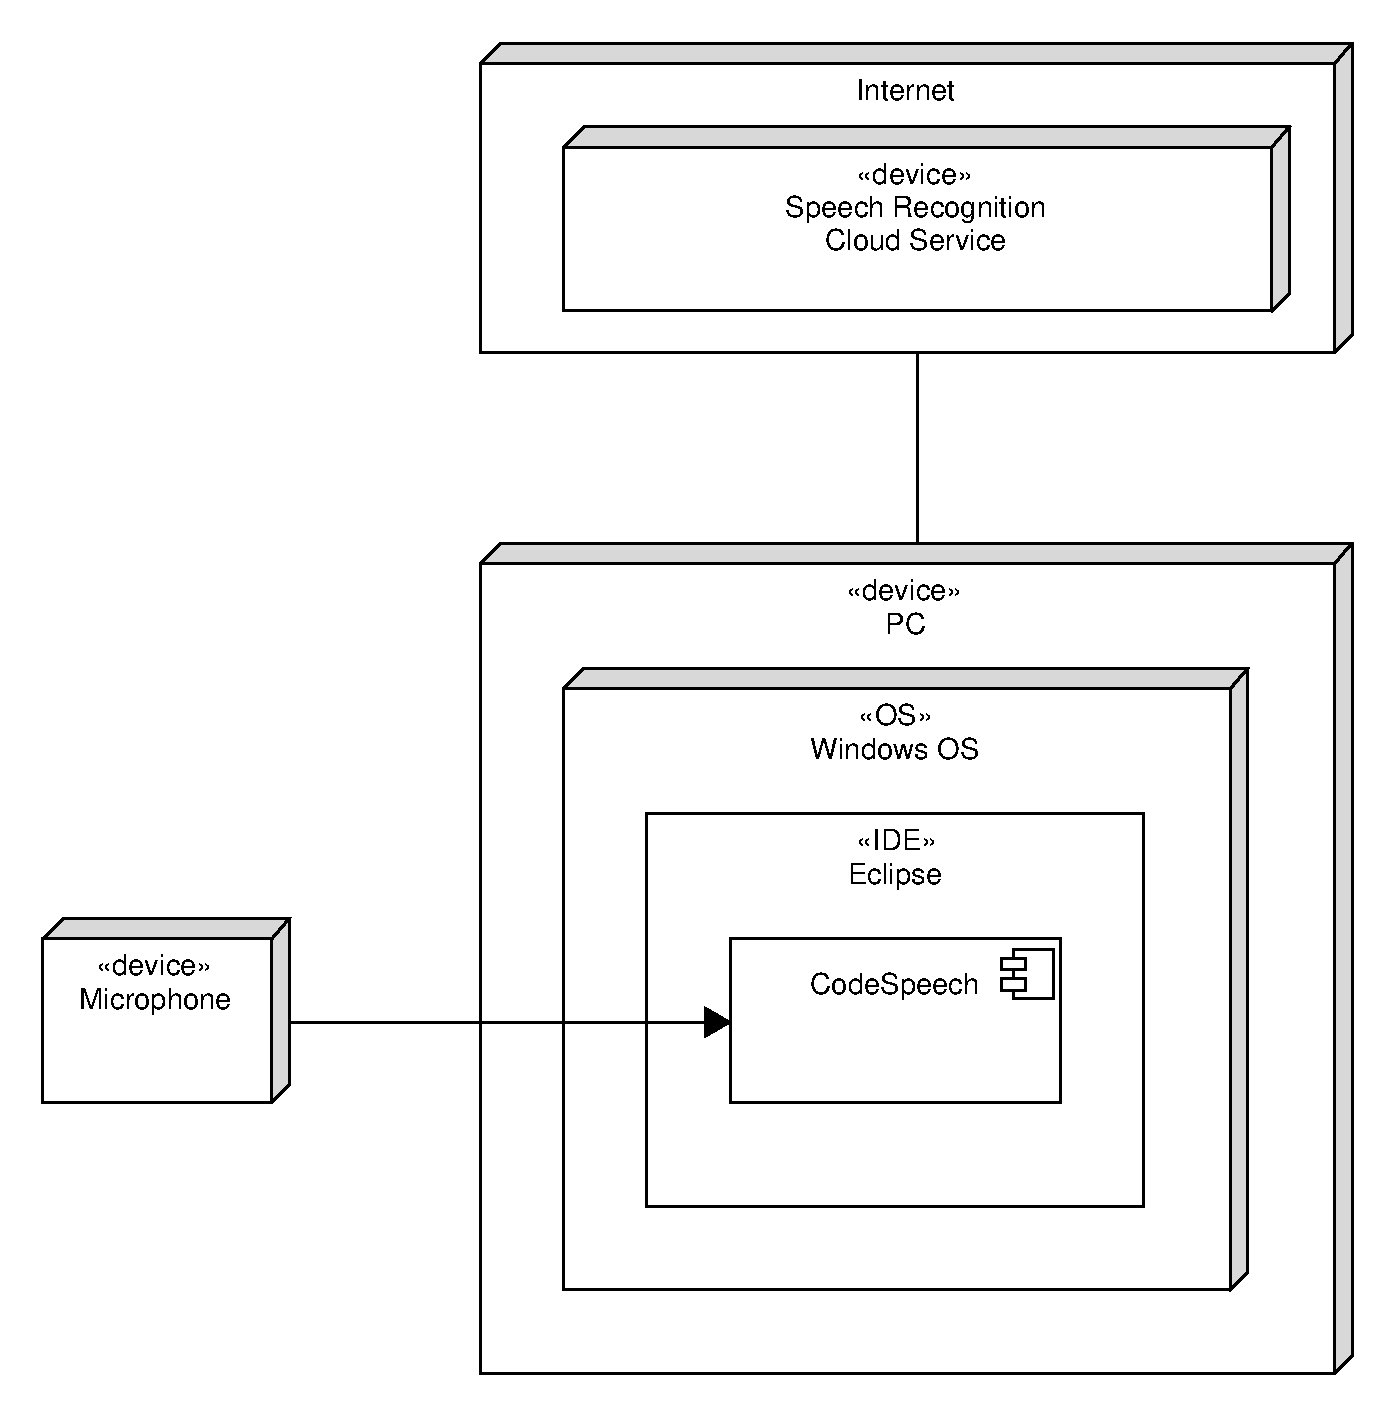
\includegraphics[width=\textwidth]{images/SystemDiagram.pdf}}
\caption{ System diagram.  }
\label{fig:systemDiagram}
\end{figure}

\subsection{Interface}

In order to have control over the plugin a button will be put into the toolbar menu. Clicking the button will toggle on and off programming by voice. Location of the button is presented in Fig. \ref{fig:toggleButton}. This method is a temporary solution because it still requires the use of mouse. In the future this way of interaction should be possibly replaced by activating via a specific command to decrease the need of using a mouse to zero. That will require to start up the programming by voice and activate microphone from the initialization of the IDE and wait for a specific voice command, such as \eg ``start voice programming''. Similarly ``stop voice programming'' would turn the main functionality off.  

\begin{figure}[hbt!]
    \centering
    \fbox{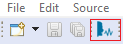
\includegraphics[width=.6\textwidth]{images/ToggleButton.png}}
    \caption{Toggle button (in red frame) added to the menu to enable and disable programming by voice.}
    \label{fig:toggleButton}
\end{figure}

There exists an alternative way to control the plugin without the need of a mouse, namely a ``mouse grid'' tool that some of the available SR software, such as Windows SpeechRecognition, provide. Users can activate a grid that divides a screen into nine sections, and by speaking the number of a section where their interest lies, the grid scales and appears in that section as presented in Fig. \ref{fig:mouseGrid}. When one cell of a grid lies entirely in the position which they want to perform click on, it can be done simply speak a number of this cell and end with ``click'' word. That is a general idea behind this function, details might differ from one tool to another. After CodeSpeech is activated, external SR tool can be turned off. Stopping voice programming works analogically.


\begin{figure}[hbt!]
    \centering
    \fbox{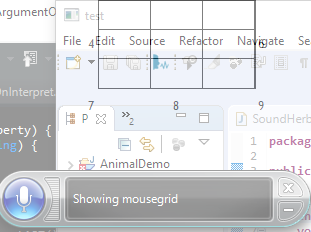
\includegraphics[width=.7\textwidth]{images/MouseGrid.png}}
    \caption{Mouse grid tool - alternative to the use of mouse build into Windows 10 SR.}
    \label{fig:mouseGrid}
\end{figure}

In addition a dialog box was introduced in the first iteration of the project in order to allow for introducing commands via text. This allows skipping the speech recognition phase and is to be used for debugging. This dialog is not planned to be used in the final version of the plugin. Fig. \ref{fig:debugDialog} depicts the command dialog box.

\begin{figure}[hbt!]
    \centering
    \fbox{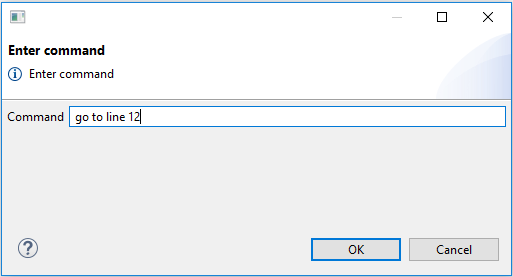
\includegraphics[width=.9\textwidth]{images/CommandDialogBox.PNG}}
    \caption{Command Dialog box that allows manual entry of commands.}
    \label{fig:debugDialog}
\end{figure}
\chapter{Implementation}
\label{cha:Implementation}

In this chapter the most important details about the implementation are revealed. The general idea behind the workflow is described and presented in the form of sequence diagrams. Class and package diagrams show basic architecture of the implementation, and the most important structures are discussed with a few interesting source code listings.

\section{Packages}
As could be seen in the previous section, whole plugin is divided into three main parts: plugin management, speech recognition and interpretation. Classes important for each particular part are placed in the respective packages. The package structure can be seen in Fig. \ref{fig:packageDiagram}. 

\begin{figure}[hbt!]
    \centering
    \fbox{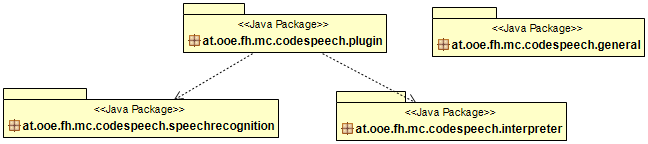
\includegraphics[width=0.9\textwidth]{images/PackageDiagram.png}}
    \caption{Basic package structure and dependencies.}
    \label{fig:packageDiagram}
\end{figure}

\subsection{\textit{general} package}
The \textit{general} package contains elements of the system that are common for every other package. Its subpackage \textit{exceptions} is a place for classes that can be used to throw exceptions. As for now there exist two of those, namely \texttt{NotImplementedException} and \texttt{InvalidNumberException}. The \textit{events} subpackage consists of \texttt{Even<T>} abstract class that is a parent of any other implementation of an event to be handled by \texttt{EventHandler}. An example of a child event is \texttt{OnInterpretationFinishedEvent} of \textit{interpreter} package. Finally, \textit{utils} subpackage has two static utility classes that allow operations on strings (\texttt{StringUtils}) and conversion of word to number (\texttt{WordToNumber}).


\subsection{\textit{plugin} package}
The \textit{plugin} package consists of elements that are related to the management of a plugin. It contains the most important \texttt{PluginManager} class, as well as static helper classes used for handling of operations performed on text editors, package explorer, abstract syntax tree and for global search functionality. These static classes are named \texttt{EditorManager}, \texttt{PackageExplorerManager}, \texttt{ASTManager} and \texttt{Searcher} respectively and are held in \textit{utils} subpackage. Another class contained in \textit{plugin} package is \texttt{ToggleSpeechRecognition-} \texttt{Handler}, which turns on or off active listening when menu button is toggled. For debugging purposes an additional dialog box was added to the IDE, which allows to skip speech recognition part and enter the command in the text form. The dialog is implemented as \texttt{CommandDialog}. By pressing the OK button an \texttt{EnterCommandHandler} is triggered. All three of these are part of the plugin and therefore they can also be found in the subpackage \textit{menu}.

\subsection{\textit{speechrecognition} package}
As the name suggests this package holds implementation of speech recognition elements. The most important one is \texttt{SpeechRecognizer} abstract class, which enables usage of many different SR toolkits. Currently there are three different classes utilizing different APIs that inherit from it, namely \texttt{Sphinx4SpeechRecognizer}, \texttt{PocketsphinxSpeechRe-} \texttt{cognizer} and \texttt{GoogleSpeechRecognizer}. These were put into subpackages \textit{cmusphinx} and \textit{googlespeech}. To change between SR technologies a specific \texttt{Enum} value of \texttt{SREngine-} \texttt{Type} has to be passed into the \texttt{SpeechRecognitionFactory}. The factory initializes and returns specified \texttt{SpeechRecognizer} object. Selection of SR toolkit is not available from the user side, by default \texttt{GoogleSpeechRecognizer} is returned.  \texttt{SpeechRecognitionLi-} \texttt{stener} interface which provides handling methods for recognition events is also present in this package, together with the event classes. These children of \texttt{Event<T>} class are found in \textit{events}. \texttt{Microphone} class is used for management of audio recording, therefore is a part of this package.

\subsection{\textit{interpreter} package}
The main classes of this package are \texttt{Interpreter}, \texttt{InterpreterContext} and \texttt{Command}. \texttt{InterpreterListener}, which provides a way to handle interpretation events can also be found in here. For now only one such event exists, namely \texttt{OnInterpretatioFinished-} \texttt{Event} placed inside \textit{events} subpackage. The \textit{grammar} subpackage is where ANTLR generated classes are being kept. Every keyword listener that extends \texttt{BaseKeywordListener} (including \texttt{BaseKeywordListener} itself) has been placed in \textit{listeners} subpackage. \texttt{Opera-} \texttt{tion} interface together with its implementations can be found in \textit{operations}. They provide methods that consist of logic for performing specific actions, such as creation of a structure, navigation \etc Therefore, according to usage they have been separated into three categories that exist so far: \textit{creation}, \textit{modification} and \textit{navigation}. In order to ensure creation/modification of a proper programming structures, their representation has been introduced in a form of models. They all extend \texttt{Model} abstract class and can be found \textit{models} subpackage. Examples of such models are \eg \texttt{ClassModel}, \texttt{MethodInvocationModel} or \texttt{ConditionalModel}.


\section{Most important classes and interfaces}

In Fig. \ref{fig:classDiagram} one can find class diagram presenting the most important classes together with their relations. Many of these classes rely on other ones that are not depicted in here to ensure readability of the graph. Some of them will be mentioned, described or presented on another images further on. In the center of the graph with yellow color there is \texttt{PluginManager}. On its left side, depicted in green there are classes responsible for interpretation and on the right with blue color, those that take care of speech recognition. For the sake of simplicity only one subclass of \texttt{BaseListener}, \texttt{Model} and one implementation \texttt{Operation} are depicted. It is to show an example of how these classes are related. The relationships of other children are analogous.

\begin{sidewaysfigure}
    \centering
    \fbox{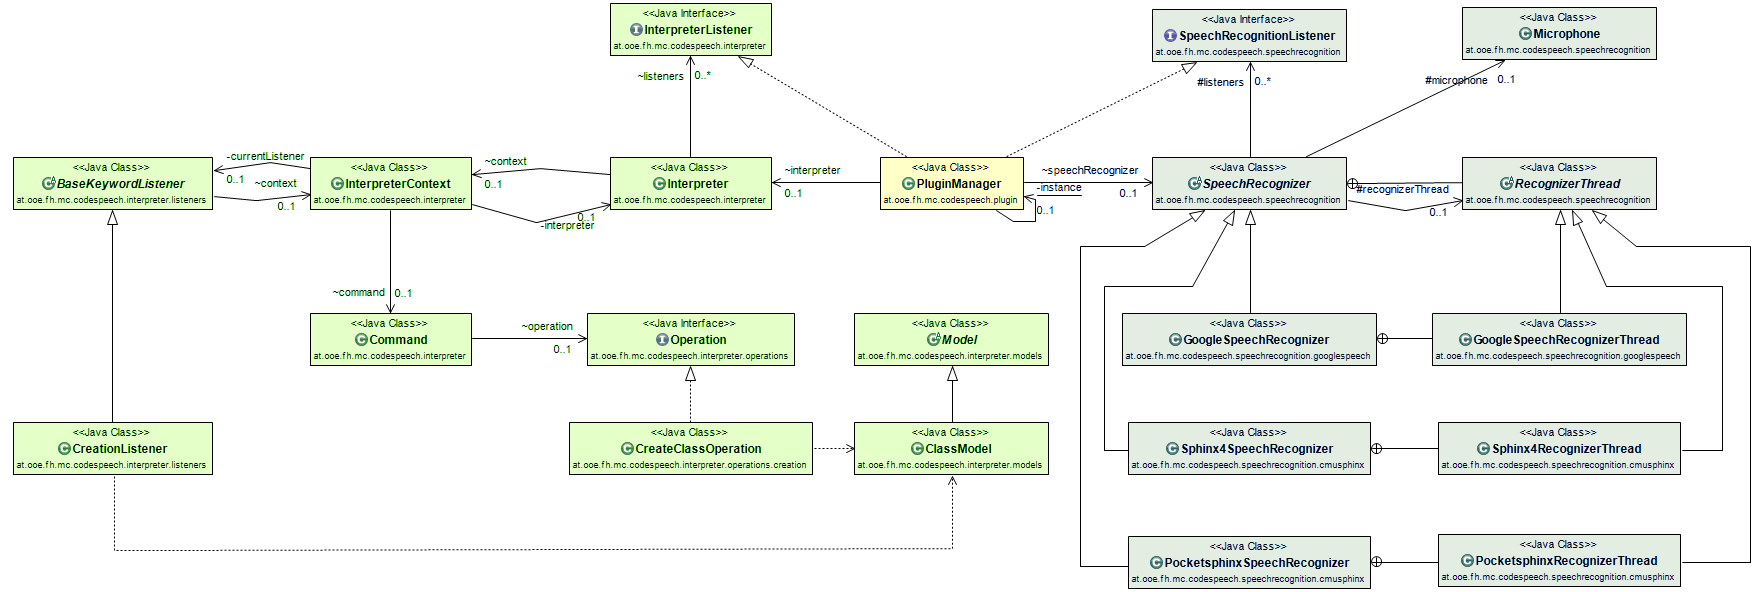
\includegraphics[width=\textwidth]{images/ClassDiagram.png}}
     \caption{Class diagram representing the most important classes and their relations.}
    \label{fig:classDiagram}
 \end{sidewaysfigure}


\subsection{PluginManager}

\texttt{PluginManager} is the heart of the plugin (usually called ``Activator'' in official documentation of PDE development). It extends \texttt{Plugin} class, which is a part of OSGi framework. Its \texttt{start} method is called the first time the plugin is initialized, which happens whenever any element of plugin is required for the first time. It is there, where all necessary objects are created. Additionally, \texttt{PluginManager} implements two interfaces created by the author, namely \texttt{SpeechRecognitionListener} and \texttt{InterpreterListener}. As the names suggest, these are the interfaces that allow handling of events related to recognition of speech and text interpretation respectively. During initialization of the plugin \texttt{Interpreter}, as well as a \texttt{SpeechRecognizer} is created. \texttt{PluginManager} also implements \texttt{IPartListener2} in order to get notified in case of any change in text editors. So far this is utilized only to keep track of currently opened editor.

\subsection{SpeechRecognizer}
\texttt{SpeechRecognizer} is an abstract class and a parent of \texttt{Sphinx4SpeechRecognizer}, \texttt{PocketsphinxSpeechRecognizer} and \texttt{GoogleSpeechRecognizer} which utilize different SR toolkits. It contains \texttt{Microphone}, \texttt{EventHandler}, \texttt{Mode} and \texttt{RecognierThread} instances, and also a list of \texttt{SpeechRecognitionListeners}. It provides methods to start and stop audio listening. As it is implemented now, three modes of recognition are possible: continuous speech, based on grammar and based on keyphrases. Only CMUSphinx recognizers provide a way for grammar-based recognition, and only PocketSphinx API can recognize in keyphrase mode. Implementation uses only continuous speech as for now. If any new SR toolkit is to be used, simply a new class has to inherit \texttt{SpeechRecognizer} and use its API in there. 
\texttt{Microphone} is responsible for gathering audio data, \texttt{Mode} is an enumeration type and its instance helps to keep track of current recognition mode.

\subsection{RecognizerThread}
\texttt{SpeechRecognizer's} inner class \texttt{RecognizerThread} extends \texttt{Thread} and it is in its \texttt{run} method where the main process of recognition is performed. This class has to be extended as well when new SR toolkit is being implemented. The most important to override are three methods: \texttt{beforeRecognition}, \texttt{recognize} and \texttt{afterRecognition}. Starting from the beginning, \texttt{beforeRecognition} is where all operations that are mandatory just before the recognition are performed. In \texttt{recognize} method the actual recognition logic is done. Finally, \texttt{afterRecognition} is where all of the post recognition operations, such as changing state to finished or breaking a connection need to be placed to avoid problems in future recognition.

\subsection{Interpreter}
Next on the list is the \texttt{Interpreter} class. It contains \texttt{InterpreterContext}, \texttt{EventHan-} \texttt{dler} and a list of \texttt{InterpreterListener} instances. Its main functionality is in \texttt{inter-} \texttt{preter} method, which is being called upon when the recognition is done. It receives a text in a form of \texttt{String}. If the text is not empty, everything needed for parsing is set up, together with generated by ANTLR tool \texttt{GrammarParser} and \texttt{GrammarLexer}. Once everything is ready, \texttt{ParseTreeWalker} walks through a tokenized tree. Details are shown in Program \ref{list:interpretation}. Once \texttt{finish} method is called by the context, \texttt{OnInterpretationFi-} \texttt{nishedEvent} is posted.

\begin{program}[hbt!]
    \caption{Start of interpretation procedure.}
    \label{list:interpretation}
    \begin{JavaCode}
public void interpret(String utterance) {
	if(!utterance.isEmpty()) {			
		GrammarLexer lexer = new GrammarLexer(CharStreams.fromString(utterance));

		CommonTokenStream tokens = new CommonTokenStream(lexer);
		GrammarParser parser = new GrammarParser(tokens);

		ParseTreeWalker walker = new ParseTreeWalker();
		
		walker.walk(context.getCurrentListener(), parser.command());	
	}
}    \end{JavaCode}
\end{program}

\subsection{InterpreterContext}
This class was created to gather all important data throughout the process of interpretation. Its instance is passed between listeners when they change. It contains many fields such as \texttt{boolean isAbstract} or \texttt{String simpleType} that are being set when a keyword, such as ``abstract'' or ``simpleType'' respectively, was detected and the corresponding method of a listener called. Once it is known what operation is to be performed and which of these properties are important, proper object is created using these properties. Additionally \texttt{InterpreterContext} contains of \texttt{Command} object, which at the proper moment is set and at the end of interpretation process passed as an argument to the listeners by the event handler.

\subsection{BaseKeywordListener}
Inheriting from ANTLR generated \texttt{GrammarBaseListener}, \texttt{BaseKeywordListener} is an abstract parent of every other listener to be used for grammar analysis of the command. It provides common functionality for other listeners like building up \texttt{Command}, canceling if something went wrong (going back to initial state) or finalizing the process. It provides an opportunity of overriding any method that is triggered when a specific token is entered or exited. An example of such method is depicted in Program \ref{list:enterPackageKeyword}. It shows a method of \texttt{SelectionListener} activated after the keyword ``select'' was detected. Once keyword ``package'' is found, \texttt{enterPackageKeyword} method of this listener is triggered and a proper model together with operation is set up.

\begin{program}[hbt!]
    \caption{Entering ``packageKeyword'' token in \texttt{SelectionListener}.}
    \label{list:enterPackageKeyword}
    \begin{JavaCode}
@Override
	public void enterPackageKeyword(PackageKeywordContext ctx) {
		super.enterPackageKeyword(ctx);

		changeProperty(new PackageModel());
		changeOperation(new SelectPackageOperation());
	}    \end{JavaCode}
\end{program}

\subsection{Command}
\texttt{Command} is a simple but important class. It has two objects that are being set during the interpretation. First one is an instance of \texttt{Operation} and the second is \texttt{Object property}. When the command is executed, \texttt{perform} method of operation is called with the \texttt{property} object passed as argument.

\subsection{Operations}
\texttt{Operation} is an interface and each class that agrees to fulfill its contract has to implement \texttt{perform} method. Each operation is different, therefore each is implemented separately. Examples of operations are \eg \texttt{CreateClassOperation} or \texttt{ChangeReturnType-} \texttt{Operation} or \texttt{SelectAndOpenClassFileOperation}. An example of yet another operation is given in Program \ref{list:operationExample}.


\begin{program}[hbt!]
    \caption{\texttt{AddArgumentOperation} class. It can be seen that operation classes contain of only one method and nothing else. Operations use utility methods provided by \texttt{ASTManager} to perform changes to AST and by \texttt{EditorManager} to update compilation unit and place cursor into the new position.}
    \label{list:operationExample}
    \begin{JavaCode}
public class AddArgumentOperation implements Operation {

	@Override
	public void perform(Object property) throws Exception {
		if(property instanceof String) {
			ASTNode node = ASTManager.getNextNodeOfType(
		    	ASTManager.currentNode, MethodInvocation.class);
			if (node != null && node instanceof MethodInvocation) {
				AST ast = node.getAST();
				ASTRewrite rewriter = ASTRewrite.create(ast);
				ListRewrite listRewrite = rewriter.getListRewrite(
				    node, MethodInvocation.ARGUMENTS_PROPERTY);
				
				MethodInvocation methodInvocation = (MethodInvocation) node;
				SimpleName name = ast.newSimpleName((String) property);
				listRewrite.insertLast(name,  null);
			
				EditorManager.updateCompilationUnit(rewriter.rewriteAST());
				EditorManager.moveToNode(name);		
			}
				
		}
	}
}   \end{JavaCode}
\end{program}

\subsection{Models}
As mentioned before, in order to create a proper structure with correct properties models were introduced. Each model is different, depending on which AST node or program structure it represents. All models inherit a getter and setter of a \texttt{String phrase}. The reason for that is to avoid huge switch statement and to set names of certain structures, set conditions into others \etc in a unified way.

\section{Workflow}

Below, the most important parts of the working cycle are presented and described in detail. The first important part of a workflow is speech recognition, the second is interpretation. For better understanding of the activities, each of them is depicted in the form of sequence diagrams. Implementation of the most important part of speech recognition is also enlisted.

\subsection{Speech recognition}

In Fig. \ref{fig:sequenceRecognition} a sequence diagram presenting speech recognition process is shown. Once plugin is turned on (via toggle of menu button) speech recognition class starts its recognition thread. At the beginning microphone recording is started and \texttt{beforeRecognition} method called. Afterwards, functionality loops until it is interrupted. The first thing inside the loop is a check for timeout. If it did occur, an \texttt{OnTimeoutEvent} is send, if not, an input stream of a \texttt{Microphone} object is read. If audio was successfully read, \texttt{recognize} method is called. At the end of successful recognition \texttt{OnResultEvent} should be posted. The main loop is surrounded by try-catch-finally block to catch any occurring exceptions that might be thrown in the process and to ensure that \texttt{afterRecognition} is called even if something went wrong. At the end microphone has to stop its recording. The full implementation of the process can be found in Program \ref{list:recognitionRun}.

\begin{program}[hbt!]
    \caption{RecognizerThread's run method.}
    \label{list:recognitionRun}
    \begin{JavaCode}
    @Override
    	public void run() {
    		long startTime;
    		long elapsedTime;
    
    		microphone.startRecording();
    
    		beforeRecognition();
    
    		startTime = System.currentTimeMillis();
    
    		try {
    			while(!interrupted) {	
    				elapsedTime = System.currentTimeMillis() - startTime;
    
    				if(timeOut(elapsedTime)) {
    					eventHandler.post(new OnTimeoutEvent(listeners));
    					break;
    				}		
    
    				byte[] bytes = new byte[BUFFER_SIZE];
    				int numberOfBytes = microphone.getStream().read(bytes);
    
    				if(numberOfBytes > 0) {					
    					recognize(bytes, numberOfBytes);
    					startTime = System.currentTimeMillis();
    				}
    			}
    		} catch (Exception exception) {
    			exception.printStackTrace();
    		} finally {
    			afterRecognition();
    			microphone.stopRecording();	
    		}
    
    	}    \end{JavaCode}
\end{program}

\begin{sidewaysfigure}
    \centering
    \fbox{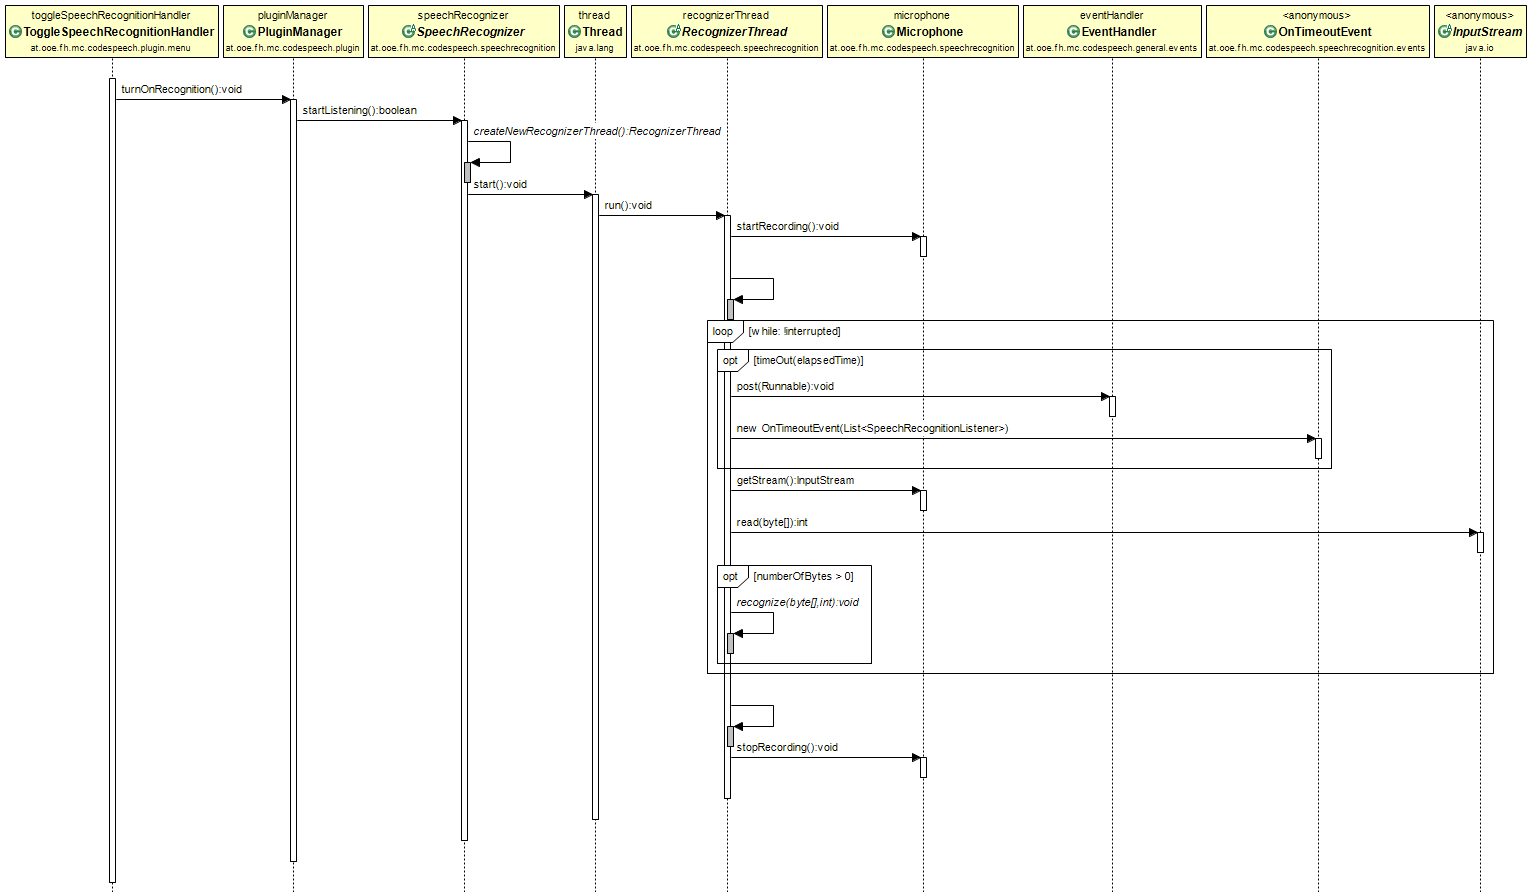
\includegraphics[width=\textwidth]{images/SequenceRecognition.png}}
    \caption{Sequence diagram showing process from start to speech recognition.}
    \label{fig:sequenceRecognition}
\end{sidewaysfigure}

\subsection{Interpretation}

Once the sentence is recognized, an \texttt{OnResultEvent} event is triggered and the utterance is sent to all listeners. The main one is \texttt{PluginManager} class, which delegates recognized text to \texttt{Interpreter}. An example of interpretation procedure is depicted as sequence diagram in Fig. \ref{fig:sequenceInterpretation}. Once \texttt{interpret} method of \texttt{Interpreter} object is called, it initializes all the necessary objects needed for ANTLR parsing and starts walking through the parsed tokens. Interpretation always starts with an \texttt{InitialListener} (all listeners extend \texttt{BaseKeywordListener}), which first listens to the keyword determining operation type and then delegating parsing to another listener accordingly. Listeners can be viewed as the state, which provides different functionality depending on the current situation. Once the listener is changed the interpretation continues. During the whole process, \texttt{InterpreterContext} object is being built up, together with its \texttt{Command} object. Once the whole text has been analysed, an \texttt{OnInterprataionFinished} event is triggered and \texttt{InterpreterListeners} are notified. Here again, \texttt{PluginManager} is a main subscriber. Once receiving a notification, \texttt{PluginManager} performs specific action using generated \texttt{Command}.

\begin{sidewaysfigure}
    \centering
    \fbox{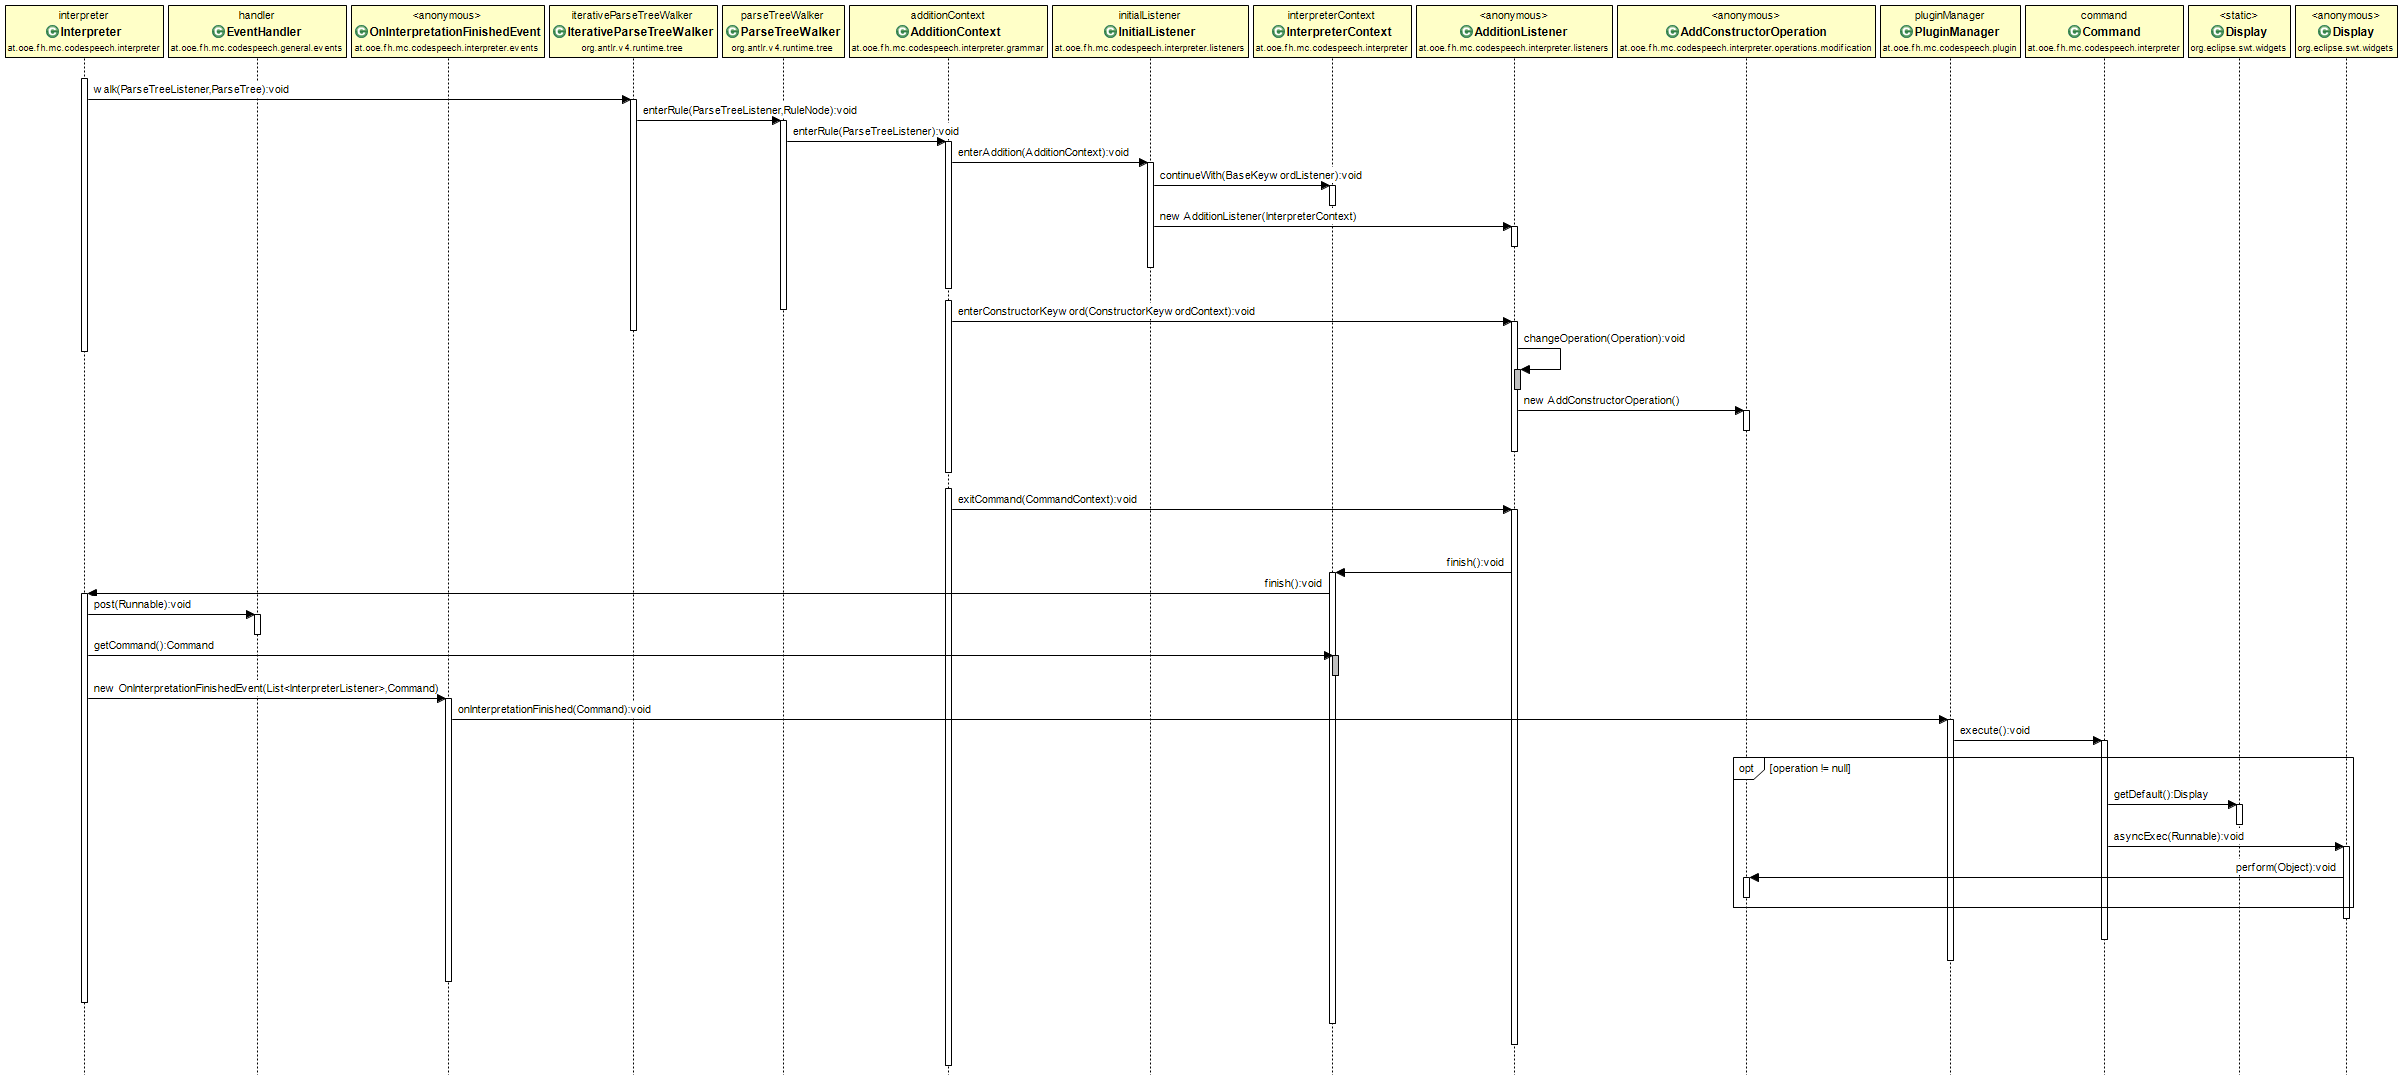
\includegraphics[angle=180,width=\textwidth]{images/SequenceInterpretation.png}}
    \caption{Sequence diagram showing interpretation from start of walking through parsed text to execution of operation.}
    \label{fig:sequenceInterpretation}
\end{sidewaysfigure}

\subsection{Performing operation}

Operations have different responsibilities depending on action they need to execute. Some modify AST by adding new node, deleting or changing one, others select an element in the package explorer or navigate in the currently open editor. In order to perform its task on IDE \texttt{Operation} has to use Eclipse API. Some common functionality has been derived and placed into utilization classes such as \texttt{EditorManager}, \texttt{ASTManager} and \texttt{PackageExplorerManager}. In Fig. \ref{fig:sequenceOperation} a sequence diagram showing the workflow of inserting new \textit{if statement} is shown as an example.

\begin{sidewaysfigure}
    \centering
    \fbox{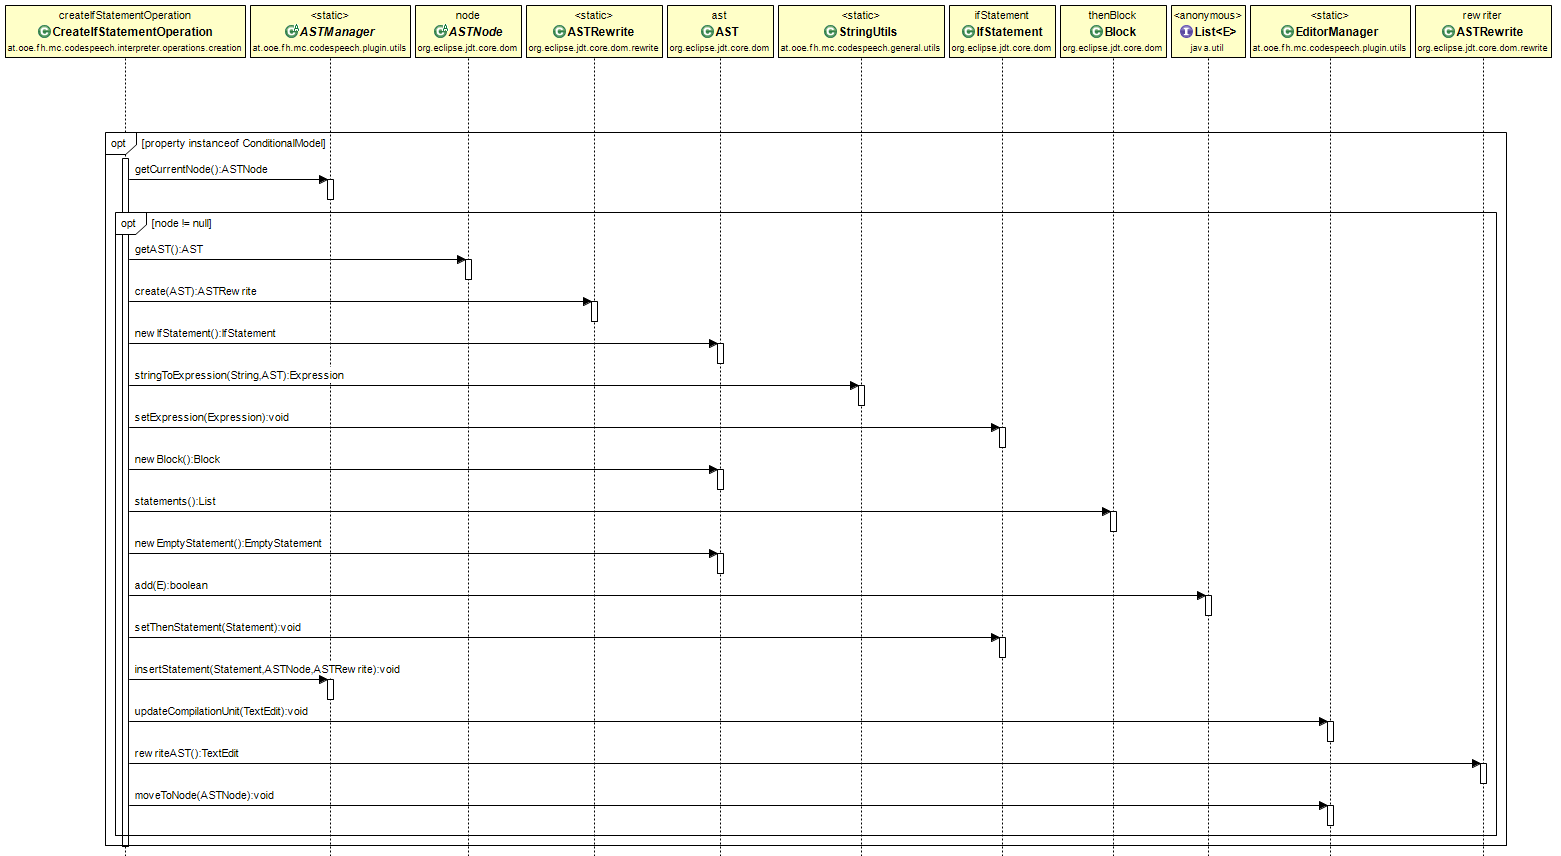
\includegraphics[width=\textwidth]{images/SequenceOperation.png}}
    \caption{An example of operation workflow for operation modifying AST. The use of utilization static classes such as \texttt{StringUtils}, \texttt{ASTManager} and \texttt{EditorManager}.}
    \label{fig:sequenceOperation}
\end{sidewaysfigure}

\section{Implemented features}
At the current state CodeSpeech provides a limited amount of functionalities. In this section their a complete list can be found. Features have been divided into three groups: creation, modification and navigation and they are presented in Tab. \ref{tab:creationFeatures}, Tab. \ref{tab:modificationFeatures} and Tab. \ref{tab:navigationFeatures} respectively. Some of the most interesting features are described in more detail in the following subsections.

\subsection{Error Correction}
Currently the only error correction measure that works is inside the text editor. Since programming is mostly happening in it, it therefore covers most of the cases. By giving the command ``undo last'' the last performed action will be reversed. It can come in handy at times, because the alternative is to delete the whole structure and create it anew. This of course would add to delay and frustration of the user. Unfortunately, when a wrong element is created in the package explorer, such as a project, package or a compilation unit with wrong name it has to be removed and the process repeated.

\subsection{Free Speech Mode}

Unfortunately, because of time limits the current state of the project does not allow for creation of the whole program from scratch. In some cases the use of mouse and keyboard is inevitable. In order to limit this need to the absolute minimum, a special free speech mode was added to the implementation. This mode is the latest addition and is entirely experimental. It allows to enter text as it is recognized, with a small modifications to the text, such as changing it to lower case and removing the spaces between words separated by periods (which is supposed to make up for the lack of nested OOP calls, such as \texttt{System.out.println()}). This mode could be turned on via ``enter free speech'' command, and analogically, exited by saying ``exit free speech''. To ensure easy error correction in case of wrong recognition, a possibility to reverse last change was kept for this mode.

\section{Addition of new functionality}

Once the design of the basic structure was established, adding new functionalities became quite easy. An example will be given on one of the latest features added into the program, which allows entering text straight into the editor. 

Basically whenever a new feature is to be implemented, what has to be done first is the addition of a new parser rule, with which the action is to be called, to the grammar. Fig. \ref{fig:grammarChange} depicts newly inserted phrases. When modification is done and the grammar is ready, ANTLR files have to be generated as described in the official documentation (or in \textit{Tools} chapter). 

\begin{figure}[hbt!]
    \centering
    \fbox{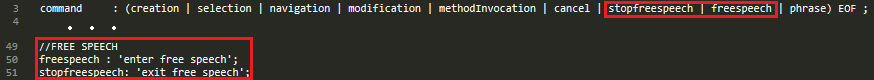
\includegraphics[width=1\textwidth, angle=0]{images/AddingNewPhrase.png}}
    \caption{Part of grammar. The text in red frame has been added to provide new commands.}
    \label{fig:grammarChange}
\end{figure}

For every new parser rule added, the generated files provide new methods for entering and exiting the rule during parsing. In this example such methods are \texttt{enterFreespeech}, \texttt{exitFreespeech},  \texttt{enterStopfreespeech} and \texttt{exitStopfreespeech}. These are inserted into \texttt{GrammarListener} interface and will become available to every other custom listener that implements it (in the current implementation all listeners do through the inheritance of \texttt{BaseKeywordListener}). Whenever it is necessary, a new listener ought to be created. This step can be skipped if one of the existing listeners can be used, \eg if creation of new structure is to be added, an already existing \texttt{CreationListener} will most likely be extended. That is not the case now and so \texttt{FreeSpeechListener} must be created. It is supposed to be activated on \texttt{enterFreespeech}, so this method is overridden in the \texttt{InitialListener}. In there the current listener (state) of the \texttt{InterpreterContext} is changed to the new one like shown in Program \ref{list:enterFreeShpeech}. 

\begin{program}[hbt!]
    \caption{Replacing the current listener to \texttt{FreeSpeechListener} triggered by ``enter free speech'' command.}
    \label{list:enterFreeShpeech}
    \begin{JavaCode}
	@Override
	public void enterFreespeech(FreespeechContext ctx) {
		super.enterFreespeech(ctx);
		context.continueWith(new FreeSpeechListener(context));
	}   \end{JavaCode}
\end{program}

\texttt{FreeSpeechListener} needs to do three things: put text into the editor, be able to reverse changes and go back to the initial state. Adding new text to the editor is new functionality, therefore a new \texttt{Operation} is required. This operation should take raw text as an input, rework it and add it to the editor. The resulting \texttt{FreeSpeechOperation} can be seen in Program \ref{list:freeSpeechOperation}. 

\begin{program}[hbt!]
    \caption{Implementation of new functionality, which works on string and puts it into the current line in the editor.}
    \label{list:freeSpeechOperation}
    \begin{JavaCode}
public class FreeSpeechOperation implements Operation {
	@Override
	public void perform(Object property) throws Exception {
		if(property instanceof String) {
		    EditorManager.enterText(((String) property).replace(". ", "."));
		}
	}
}  \end{JavaCode}
\end{program}

The next feature available from this state is change reversal. The \texttt{UndoOperation} already exists and is simply be reused. Finally, on command ``exit free speech'' the state is changed to the initial one (meaning changing the current listener to \texttt{InitialListener}). Property and operation are cleared. Whole \texttt{FreeSpeechListener} can be seen in Program \ref{list:freeSpeechListener}. That concludes the process of adding new functionality. Details might vary depending on how complex is the command, how many parser rules it consists and so on. Sometimes using more than one listener might be a viable solution to perform a task. 
\begin{program} [hbt!]
    \caption{Implementation of free speech state that is being triggered by three different commands.}
    \label{list:freeSpeechListener}
    \begin{JavaCode}
public class FreeSpeechListener extends BaseKeywordListener {
    ...
	@Override
	public void enterPhrase(PhraseContext ctx) {
		super.enterPhrase(ctx);
		changeProperty(ctx.getText());
		changeOperation(new FreeSpeechOperation());
	}
	@Override
	public void enterStopfreespeech(StopfreespeechContext ctx) {
		super.enterStopfreespeech(ctx);
		changeProperty(null);
		changeOperation(null);
		context.continueWith(new InitialListener(context));
	}
	@Override
	public void enterUndo(UndoContext ctx) {
		super.enterUndo(ctx);
		changeOperation(new UndoOperation());
	}
} \end{JavaCode}
\end{program}

\begin{table}[hbt!]
    \caption{List of functionalities from creation group.}
        \label{tab:creationFeatures}
        \centering
        \setlength{\textwidth}{5mm} % separator between columns
        \def\arraystretch{1} % vertical stretch factor
        \begin{tabular}{|p{3cm}|p{6,25cm}|p{4cm}|}
            \hline 
            \emph{Functionality} & \emph{Details} & \emph{Example command} \\
            \hline
            Create Java project & Given name is in format of Pascal case. & create project project name  \\
            \hline
            Create package & Given name is in Java  convention format. & create package package name  \\
            \hline
            Create class & Given name is in Java format of Pascal case. & create class class name  \\
            \hline
            Create class / interface file & Given name is in Java format of Pascal case. Can be abstract, final, with access modifier. & create abstract class class name  \\
            \hline
            Create method body & Given name is in Java format of Camel case. Can be abstract, static, final, with access modifier. & create public static method main method  \\
            \hline
            Create variable & Given name is in Java format of Camel case. Can be static, final, with access modifier. So far allows primitive and simple types and arrays thereof. & create integer count \newline create array list named list \newline create array of string named string list \\
            \hline
            Create if statement & Allows for simple prefix, infix and postfix conditions. Does not allow method invocations, complex conditions or String comparison. & create integer count \newline create if count is greater than zero\\
            \hline
            Create else statement & Allows adding else of else if statement. Conditions restricted as for if statements. & create else  \\
            \hline
            Create while loop & Conditions restricted as for if statements. & create while not true  \\
            \hline
            Create method invocation & Allows to call a method on an object, class or without. & call get state \newline on out call print \newline on class integer call to string\\
            \hline
        \end{tabular}
\end{table}

\begin{table}[hbt!]
    \caption{List of functionalities from modification group.}
        \label{tab:modificationFeatures}
        \centering
        \setlength{\textwidth}{5mm} % separator between columns
        \def\arraystretch{1} % vertical stretch factor
        \begin{tabular}{|p{3cm}|p{6,25cm}|p{4cm}|}
            \hline 
            \emph{Functionality} & \emph{Details} & \emph{Example command} \\
            \hline
            Add argument to method call   & Possible is adding one only argument at a time.    & add argument name  \\
            \hline
            Add constructor        & Adds constructor to the class. Allows only public constructor (by default). & add constructor  \\
            \hline
            Add parameter to method body & Possible is adding only one argument at a time. Allows primitive type, simple type and array thereof.  & add parameter double result \newline add parameter array of class name named parameter name  \\
            \hline
            Assign value & So far possible is only assignment of a simple name to simple name. & simple name assign another simple name \\
            \hline
            Change return type &  Changes return type of the method body. Allows primitive type, simple type and array thereof. & change return type to double\\
            \hline
            Delete argument &  Deletes argument on a given position. Only one at a time is possible. & delete argument two\\
            \hline
            Delete node &  Deletes current AST node. It can be variable definition, else statement or whole method. & delete line\\
            \hline
            Delete parameter & Deletes parameter on a given position. Only one at a time is possible. & delete parameter one\\
            \hline
            Delete project & Requires a project to be selected. & delete project\\
            \hline
            Delete package & Requires a package to be selected. & delete package\\
            \hline
            Delete class/interface file &  Requires a class/interface to be selected. & delete class\\
            \hline
            Extend class &  Adds extends statement to the class. & extend parent class\\
            \hline
            Implement interface &   Adds implements statement to the class & implement interface\\
            \hline
            Free speech & Allows addition of recognized text as it is. & enter free speech \newline text to put \newline exit free speech \\
            \hline
            Initialize variable & Adds initialization depending on type. Can be a number, simple type or text in quotes for String. & initialize to text \\
            \hline
            Add return statement & Adds return statement for return type. Allows numbers and simple types. & return variable name \\
            \hline
            Undo last action & Reverts last change in the editor. & undo last \\
            \hline
        \end{tabular}
\end{table}

\begin{table}
        \caption{List of functionalities from navigation group.}
        \label{tab:navigationFeatures}
        \centering
        \setlength{\textwidth}{5mm} % separator between columns
        \def\arraystretch{1} % vertical stretch factor
        \begin{tabular}{|p{3cm}|p{6,25cm}|p{4cm}|}
            \hline 
            \emph{Functionality} & \emph{Details} & \emph{Example command} \\
            \hline
            Line navigation & Moves cursor to given line number. & go to line 10 \newline go to 5  \\
            \hline
            Select project & Selects project in package explorer. & select project project name  \\
            \hline
            Select package & Selects package in package explorer. Project has to be selected first. In case of subpackage only its name can be given (\eg select package models can select animals.models). & select package package name  \\
            \hline
            Select and open \newline class or interface & Selects in package explorer and opens in new editor class/interface file. & select interface interface name \newline select class class name \\
            \hline
        \end{tabular}
\end{table}

\chapter{Evaluation}
\label{cha:Evaluation}

%  - result of user study, results, performance etc			
%  - describe process/use in steps with screenshots,			
%  - thoughts on development, how to make it better (recognition)			
%  - how well my initial idea worked out, what could be better			
%  -mouse clicks count (RSI)			
%  - evaluation of time using Eclipse, SR and MS SR			


After close to 400 hours spent on design and implementation, the finished prototype was created. It still does not allow to create a whole program entirely by voice, but it is ready for its first evaluation. This evaluation is not a user study per se, because it was done only by the author himself. It is therefore only an initial test of a prototype's functionality which is supposed to give an idea if the project gets closer to reaching the goal and if there is a potential worth in continuation of work. The observations arising from the test's result can also point a direction in which further development should go to, as well as it can be a foundation for a real user study that is planned in the near future.


\section{Approach}
The rationale behind the evaluation is to find out if the created system can be introduced as an alternative for the standard way of fulfilling the task of writing programs and therefore decrease the amount of mouse and keyboard usage. In order to do so, a test was carried out, the goal of which was recreation of a simple Java program using two input methods and compare the results. The two methods under test were: a common one based on typed input and cursor control, and a second one relying on voice. Because CodeSpeech is still just a prototype and not a finished product, its evaluation required partial usage of peripheral input devices in places where the necessary functionality was lacking. 

The Java program that was to be created during the test was
very simple, consisting of one interface, one abstract class implementing this interface, three classes extending the abstract one, and a main class which initialized three instances, called their methods and printed resulting text as an output to the console. All program elements can be found in Appendices \ref{appendix:soundable} - \ref{appendix:animals}, but to briefly get an idea of its complexity the class diagram is presented in Fig \ref{fig:animalDemo}. 

\begin{figure}
    \centering
    \fbox{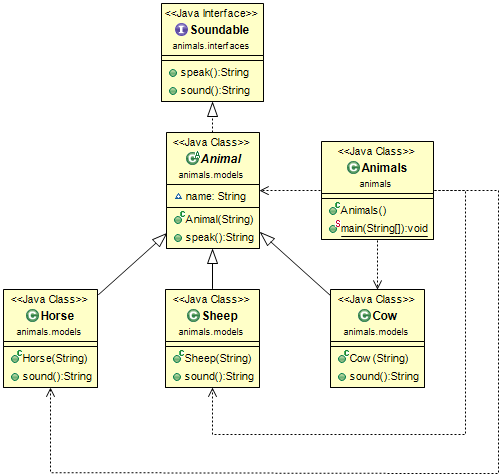
\includegraphics[width=0.9\textwidth]{images/AnimalDemo.png}}
    \caption{Class diagram of test program used to compare both input methods.}
    \label{fig:animalDemo}
\end{figure}

The workstation on which the experiment has been conducted was Lenovo Y510P laptop with Intel i7 2.40GHz processor and built in keyboard and an external optical mouse Dell DZL-MS111-L(B). The station was running Windows 10 operating system and Eclipse IDE of version 2019-06 (4.12.0). Voice recording was done by an internal microphone built into the laptop. The test was performed in English language by a non-native speaker. \\
The software tool used to record an activity of mouse and keyboard was Mousotron 12.1 \footnote{http://www.blacksunsoftware.com/mousotron.html}.
Mousotron allows to monitor different types of activities. The ones that were selected as relevant for this evaluation were:
\begin{itemize}
    \item running time,
    \item cursor distance,
    \item number of keystrokes,
    \item number of left button clicks,
    \item number of right button clicks,
    \item number of middle button clicks,
    \item number of double clicks,
    \item mouse wheel scrolls,
    \item and idle time.
\end{itemize}
Running time is measured from the beginning to the end of recording. The timer starts or stops by pressing on/off button according to the current state. Idle time measures the time in which no activity of any of the peripheral devices was detected. The delay of starting the counter was set to zero. By subtracting idle time from running time we can get the real time of keyboard and mouse usage (without distinction between them). Cursor distance monitors what distance was traveled by the cursor in either metric or English system. The distance is calculated using the size of the display and the current resolution of the screen. The display used during the test was an 18,5 inches Samsung S19A300N with resolution of 1366x768. Although this value does not give the physical distance traveled by the mouse, it still adds an important information if used in comparison between two sessions. The relation between this distance and the physical distance is proportional if the same mouse sensitivity is used. The rest of the metrics are self explanatory. Single clicks of left, right and middle button were combined to provide a single measure. The layout of the Mousotron application is presented in Fig. \ref{fig:mousotron}. 

\begin{figure}
    \centering
    \fbox{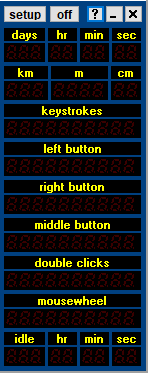
\includegraphics[width=0.2\textwidth]{images/Mousotron.png}}
    \caption{Mousotron program used to measure mouse and keyboard activity.}
    \label{fig:mousotron}
\end{figure}

In addition to input devices' metrics, another one was introduced in order to evaluate the performance of the system, namely Command Error Rate (CER). CER was measured as a ratio of the number of incorrectly interpreted (and recognized) commands (IC) versus the number of all spoken commands (N). Its formula therefore looks like this:
 $$   CER = \frac{IC}{N}. $$
 CER can be viewed as a derivative of WER of which usage did not make sense in this context. Presenting calculated WER would simply be an evaluation of speech recognition tool, and that was already done in the \textit{Tools} chapter. Instead what was preferred, was an evaluation of the performance of the whole cycle of the system, which includes interpretation, as well as recognition. The latter was made in such a way to ignore some of the words that could be in some cases accidentally introduced by SR, such as articles. Those cases should not be counted as an error if the final command was performed correctly, thus the need for CER. 
 
Once the test program was prepared and the recording software set up, the evaluation could be started. At first the program was done using the standard method, followed by the voice control method. In order for both methods to be comparable, the management of the recording had to be unified to minimize noise. The detailed description of the process backed up by screenshots can be seen in Fig. \ref{fig:steps}.
 
\begin{figure} [hbt!]
\centering\small
\begin{tabular}{@{}c@{\hspace{6mm}}c@{}} 
  \fbox{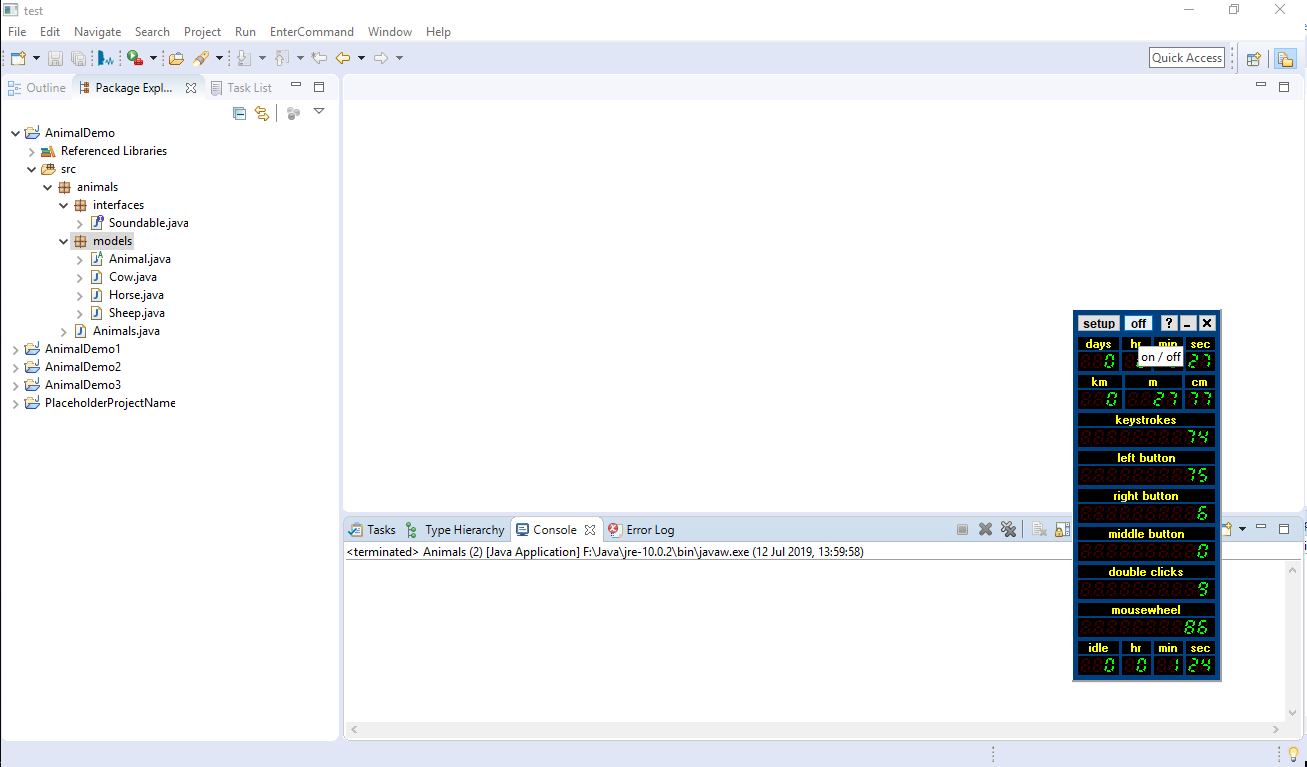
\includegraphics[width=.5\textwidth]{images/Step1.png}} &
  \fbox{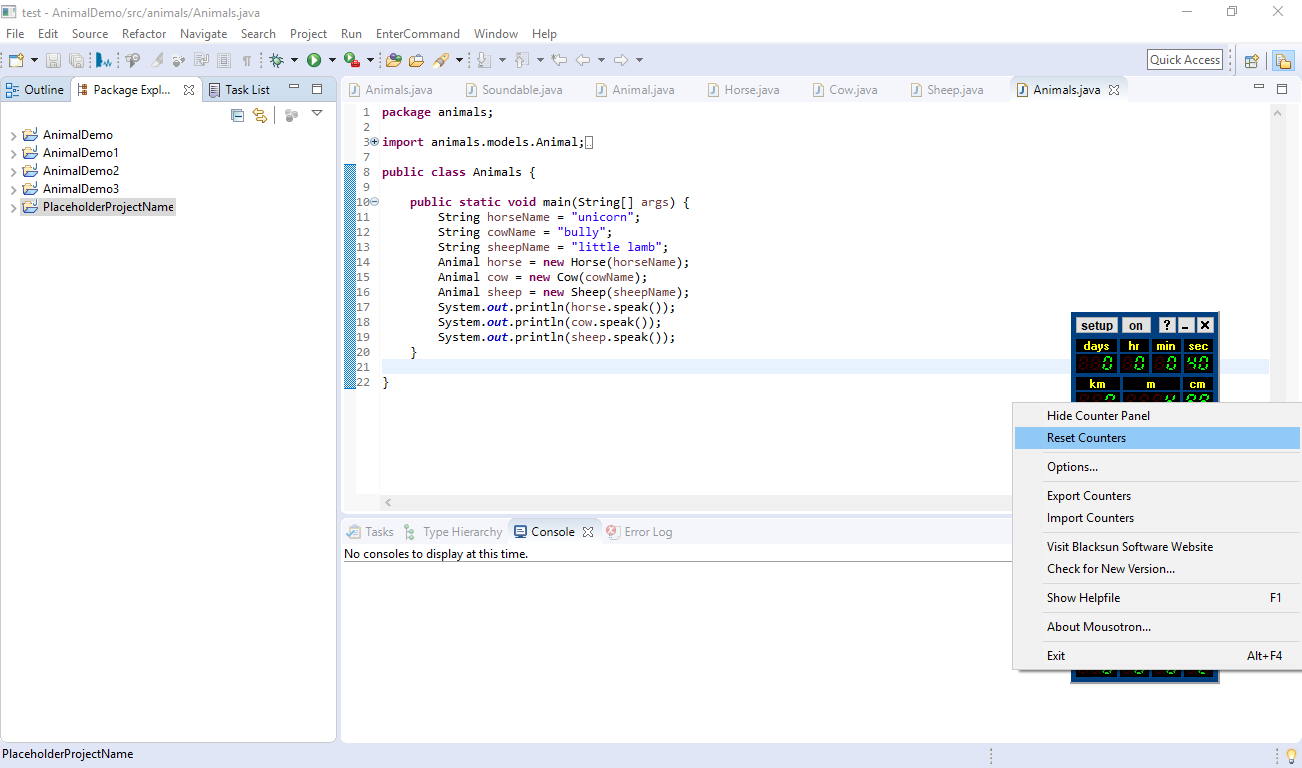
\includegraphics[width=.5\textwidth]{images/Step2.png}} 
\\
  (a) & (b)
\\[2pt]	
  \fbox{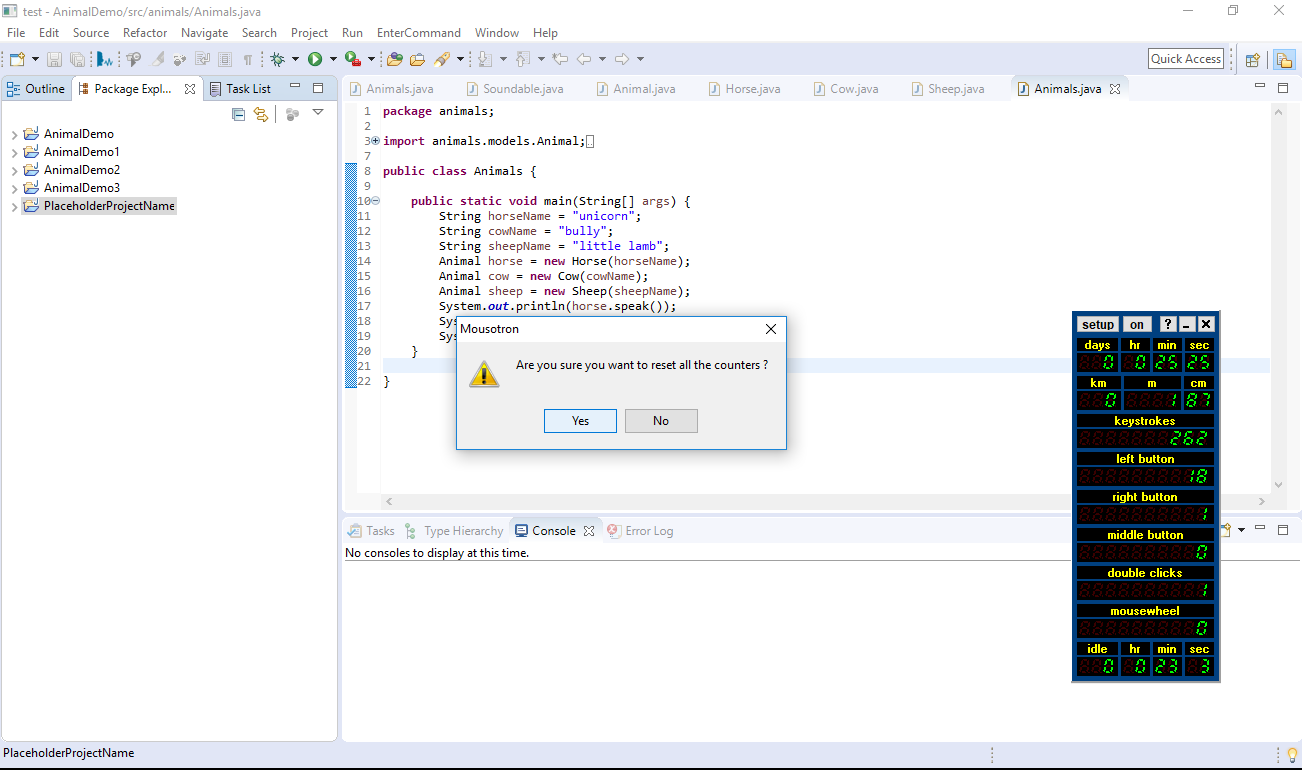
\includegraphics[width=.5\textwidth]{images/Step3.png}} &
  \fbox{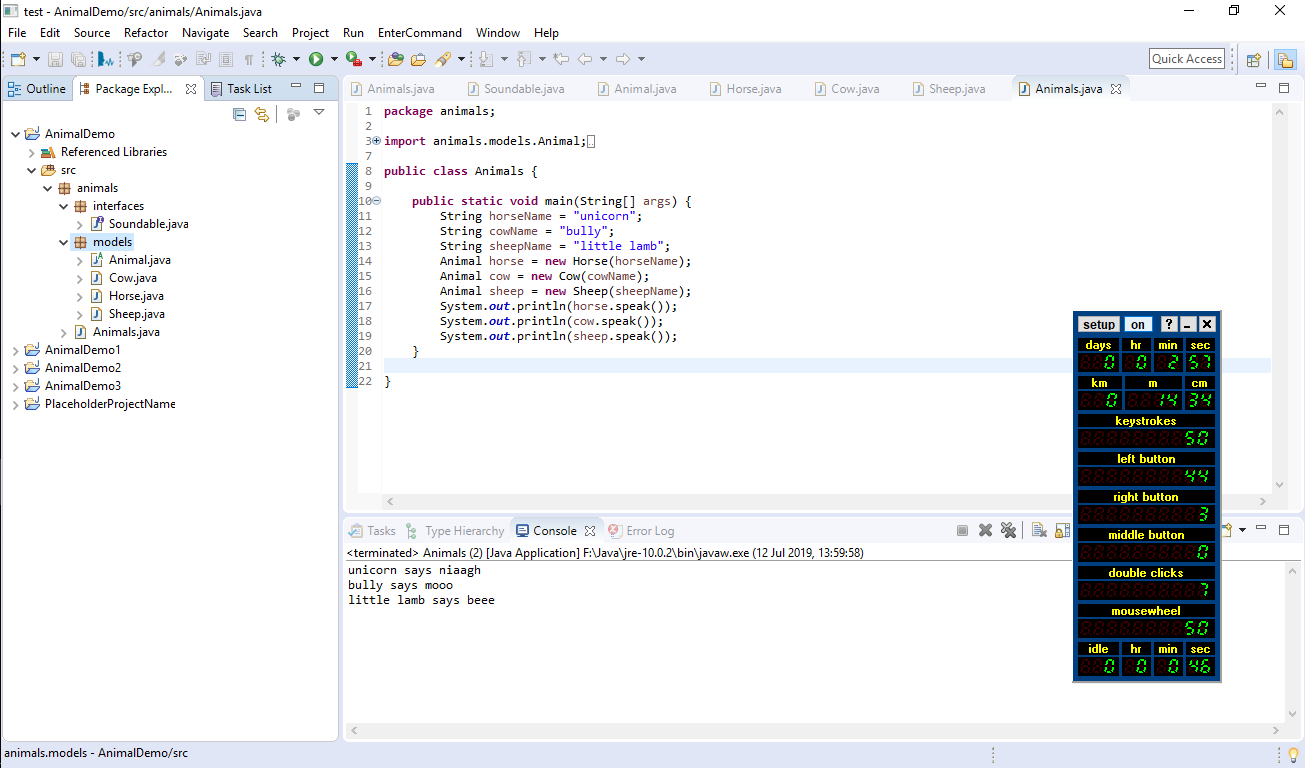
\includegraphics[width=.5\textwidth]{images/Step4.png}} 
\\
  (c) & (d)
\end{tabular}
%
\caption{ At first Mousotron and Eclipse IDE had to be both opened, visible and set to proper positions. Mousotron was set to be always on the top layer and placed in the right bottom corner of the screen to prevent covering anything considered important, to avoid the necessity of moving it during the test. This way data noise could be reduced. Once ready, the mouse and keyboard recording was started using an on/off button (a). In order to further reduce noise the counters were reset to zero via ``Reset Counters'' option (b). This made a dialog box to appear, and the counters where restarted once confirmed (c). This ensured that the initial position of the cursor was the same for both methods. After confirmation programming could begun. Finish was marked by the successful run of the program with the correct output printed into console. To stop recording, the on/off button had to be pressed again (d).}
\label{fig:steps}
\end{figure}
 
\section{Results}

The results of the evaluation of two different input methods are presented in Tab. \ref{tab:results}. In the table one can see the scores of previously selected measures. The first column titled as ``Method 1'' represents the standard way of providing input through mouse and keyboard, while the programming done mainly by voice with a support of standard input devices is titled ``Method 2''. 
As it comes to CER, the final score was 0,295 (~30\%) with a number of incorrectly interpreted commands being 67 and the total number of spoken commands was 227. 

\begin{table}
    \caption{Results of evaluation.}
    \label{tab:results}
    \centering
    \setlength{\textwidth}{5mm} % separator between columns
    \def\arraystretch{1.25} % vertical stretch factor
    \begin{tabular}{|r||c|c|}
        \hline
        & \emph{Method 1} & \emph{Method 2} \\
        \hline
        \hline
        Total time & 5 min 57 s & 24 min 54 s \\
        \hline
        Device usage time &  5 min 06 s & 1 min 55 s\\
        \hline
        Cursor distance & 887 cm & 154 cm \\
        \hline
        No. of keystrokes & 876 & 262 \\
        \hline
        No. of clicks &  84 & 17  \\
        \hline
        No. of double clicks &  19 & 1\\
        \hline
        Mouse wheel scrolls &  0 & 0\\
        \hline
    \end{tabular}
\end{table}

\section{Discussion}

The discussion about the results has been divided into three sections, focusing on different aspects: programming time, interaction with mouse and keyboard and CER. The results show that the time needed to complete a program via voice input is indeed longer, nonetheless it requires less interaction with input devices. The number of incorrect commands was relatively small, however, there is still a lot of room for improvement. More details can be read below.

\subsection{Programming time}

As it can be seen, completion of the test using Method 1 took only 5 minutes and 57 seconds, while Method 2 needed 24 minutes and 54 seconds. This in fact means that programming using CodeSpeech is around four times slower. That is a significant difference and it proves that CodeSpeech is not suitable to replace the standard method just yet. It is assumed that there are several reasons that make standard way faster. The first could be many of the options built-into IDE that speed up programming experience, such as auto-completion of text, keyboard shortcuts, problem solving suggestions, creation wizards and others. The second reason that can accelerate writing code is possibility of copying specific structures and refactoring them instead of typing them from the very beginning every time. Third reason that is suspected to have a relevance is error correction. Speech recognition systems, when recognized correctly do not introduce typos as it happens when typing. However, when recognition is not correct, trying to fix it might take longer than correcting a typo, especially when the result of recognition happens to be false more than once. Couple of times during the test a situation occurred, where one command had to be given many times over. The worst situation that has happened was in experimental free speech mode, when incorrect text was entered and the command to reverse last change was also falsely recognized. That resulted in appending incorrect text to the previous one rather than correcting an error. Now the reverse operation had to be done twice, and it could again be falsely recognized and so on. Finally, the author, who performed the test has over 5 years experience in programming, and even more in interacting with a computer using a mouse and keyboard while programming by voice is a new concept. Lots of mistakes were made, such as saying an incorrect command, stopping in the middle of the utterance to think about what comes next and forgetting about going back from free speech mode. 

\subsection{Interaction with mouse and keyboard}
Although the time required to finish the program was longer in case of Method 2, the time of mouse and keyboard usage was shorter by 3 minutes 11 seconds decreasing it to 37,6\%. Distance traveled by the cursor was shortened to 17,4\%. Method 2 required 614 less keystrokes (29,9\%) and the number of clicks and double clicks was decreased to 20\% and 5\% respectively. Mouse wheel was not used at all during the test. \\
It is clear that the usage of mouse and keyboard has been decreased quite substantially in programming by voice approach. One might argue that despite that, the increase of time needed to complete a simple program is not worth the change. The author of the thesis himself agrees with that statement, however, it is worth to remind that these are the results of the initial test and the system under evaluation is still a prototype. With the enhancement of the project and increase in functionality, usability and with better error correction a day might come when the tool becomes competitive in performance while keeping its benefits of limiting mouse and keyboard use. 

\subsection{CER}
The performance of the system could be improved by decreasing CER, on which two factors have an impact, namely accuracy of speech recognition and strictness of interpretation based on grammar. Obviously, the better the recognition, the easier is to match the grammar, however it cannot be assumed that SR will always give perfect results, that is why handling it properly by interpreter should allow some flexibility to make up for mistakes done by SR. Improving both factors will result in smaller amount of needed repetitions an error corrections and and thus, shorter time of programming. In the meantime, the next section presents some ideas about how to possibly improve the system.


\section{Ideas for improvement}
During the evaluation a couple of different ideas of how to make the program better came up. In this section some of them are presented. At the beginning the focus of the discussion is on the ideas how to make recognition better as it is obviously one of the most important factors. This at times intertwines with the ideas for improvement of interpretation. Later the section pivots to discuss how to improve usability, and finally gives examples of features that increase performance of the system.

\subsection{Interpretation of more propositions}
Speech recognition systems solve classification problem. The results that are provided are based on probability. Many SR toolkits give the whole list of potential solutions, and it is not different in the case of Google API. The output returned by the API is a list of phrases, ordered by measure of confidence. It might happen, that the correct phrase is not on the surface but rather is somewhere deeper in the list. In the current version, CodeSpeech trustfully takes the top item and do not care about the others. Perhaps interpretation could be done on all of the propositions until a correct one is found? This of course could slow down the whole cycle, unless interpretation on different phrases is done in parallel. \\
An alternative to this approach is to add an additional feature, which would allow the user to iterate through the list of propositions, \eg by running the command ``try next''. Therefore every correct recognition done at the first try would not slow down the system, and in case of incorrect one the user would have control.

\subsection{Context recognition}
Another idea focuses on adding context to the process of recognition. Google Cloud Speech-to-Text is good in recognizing continuous speech, but that does not ensure correct results in systems with limited amount of words or phrases. Programming languages themselves have restricted list of keywords. It comes to mind, that a smart idea would be to provide some context in order to increase performance and omit cases in which the phrase like ``change return type...'' is being recognized as ``Chun's restaurant...'', which of course in the programming world does not make any sense (unless Chun's restaurant is supposed to be used as a variable name). Since in CodeSpeech interpretation of recognized phrase is based on grammar, why not to use it as a context for recognition as well?  Google API does not supply such an option, but CMUSphinx tools do. The grammar it is using is different from the one used by ANTLR, so its counterpart in the form of Java Speech Grammar Format (JSGF) would need to be created. That obviously comes with some consequences, namely whenever a change is to be introduced to the grammar, both files have to be modified accordingly. Perhaps this process could be automated.  

Next concept of context based recognition relies on the third option provided by CMUSphinx, which is keyphrase recognition. Once a text file with specified phrases is created, it can then be used to trigger an action on a recognized keyphrase or single keyword ignoring the rest. That seems like a better solution in comparison to grammar, because grammar tend to be very strict, and if at least one unexpected word (such as an article) appears in the middle of a sentence, the match is not found. That makes keyphrase approach more flexible. It does sound promising, however, how it will work in practice must be investigated. 

It may be that combining one of the aforementioned approaches (or both) with continuous, free speech recognition can give even better results. CMUSphinx allows for changing between modes during run time. That could require modifying the way voice commands are given to consist of phases. Initially, the SR is set up to keyphrase detection. Once the keyphrase has been detected the mode is switched to listening for continuous speech (when the name is to be spoken), and then back. An example of recognition divided into phases could look like this:
\begin{enumerate}
    \item command ``create new public method named'' is given,
    \item keyphrase is detected, and the mode switches to free speech listening,
    \item when the user is notified, ``get current state'' name is spoken,
    \item operation creating new method of name ``getCurrentState'' is created and the mode switches back to keyphrase recognition.
\end{enumerate}
This way seems like it could again slow down the whole process a bit, but perhaps if the outcome will mean more accurate recognition, thus a decrease in the amount of repetitions needed, in the end it might turn out to actually be faster.
In order to easier operate with names that already exist in the project, perhaps a good idea is to dynamically store them in the form of separate keyphrase file. This way at the beginning of name giving phase, the recognition could be performed in keyphrase mode (just the file is changed to the one consisting of names). If relatively strong match is found, the name will be brought up, but if not then probably a new name is being given, so recognition proceeds in continuous mode. This approach could increase precision and maybe decrease error rate in code reuse.

\subsection{Combining recognition systems}
In previous subsections the usage of CMUSphinx was considered to be applied in potential future improvement work, despite the fact that in the previous sections thi technology was rejected for not being good enough. It is true that CMUSphinx's default models do not ensure a good recognition for non-native speakers. Even recommended acoustic adaptation did not provide enough improvement (would require much more adaptation than it has been done). It comes, however, with the tools to build completely new acoustic and language models based on a phonetic dictionary, which can be modified according to needs. Perhaps CMUSphinx will never be as good in continuous recognition as its commercial counterpart belonging to Google, nonetheless, it might prove good enough for the recognition of limited list of commands/words if the models are being built specifically for this purpose. Therefore the recognition of commands could be left to CMUSphinx in its more suitable modes mentioned earlier, while continuous recognition used \eg for names could be left to Google Cloud Speech-to-Text or yet another tool. The process of building all models from scratch is going to be time consuming and will require a lot of work, but it may be worth considering anyway. 

\subsection{Better error correction}
For now the only means of error correction works for the text editor, where source code is written. By saying ``undo last'' the last change in the text is reversed. In some situations, however, it might be necessary to perform reverse action more than once. In cases like this the command ``undo last'' needs to be spoken repeated couple of times. It gets even worse when this command is falsely classified and an extra text is entered. That adds to the stack of needed corrections. To make it better, it should be possible to give a number of times the reverse operation has to be made, for example ``undo last three times''. That could speed up the process. \\
Additionally other means of error correction should be implemented, such as a possibility to change the wrong name, move a structure and basically to provide more options of manipulation, as well as allowing to use some of the IDE's proposed solutions in an easy way. This should be done not only for the text editor, but also for other elements, such as package explorer. 

In SR tools such as Windows Speech Recognition, when the users are not satisfied with the inserted word, they can give a command ``correct' and are then presented with a list of options that can be selected by saying a number of a line with correct phrase. Borrowing from that a similar list could be made available to the user when an incorrect operation was performed or when it is not clear what the user is trying to do. Perhaps this solution could also be used for future reference and help the system learn to avoid similar mistakes in the future. 

\subsection{Adaptation}
Previous subsections inspired another idea. Some speech recognition systems allow for adaptation of the model with the recordings of the users to improve the results. Adding this as a feature could make sure that CodeSpeech achieves the same performance when working in different environments, voices, accents once it learns from those recordings. Whenever the users are not satisfied with the results they can start teaching mode in which they will have to read out loud a couple of sentences or perhaps specific commands. The process can be repeated a couple of times and with each improvement should be visible.

\subsection{Feedback}
Until now the focus was put on recognition, interpretation and operation execution, to make sure the system works. Currently there exists no feedback system built into the plugin, which makes it difficult to use. Whenever an error occurs or an exception is thrown, the user is not notified about that fact and therefore is unaware of why no action was performed or what he/she did wrong. Even if no error occurred, but simply the recognition was incorrect and nothing happens the user does not know the reason for it. A way to give back information of the current status should be implemented. Feedback system could be a text window (similar to the console) that displays either the recognized text, some details about performed action (if any) or simply an information that the system did not understand or wrong action was undertaken. 

\subsection{Improve voice control experience}
Ideally, the end product's input is going to be flexible enough to invoke one operation with different sentences that have the same meaning in English. If this goal turns out to be hard to reach, maybe it can be worth to consider giving the users the possibility to define their own commands for each action. All keywords could be presented in table form in which respective words could be overwritten. After the modification the program reacts to different phrases.
Despite which option will end up being in the finished product, it should be possible at any time for the user to open a list of phrases that are available in the current context. Even the author had to go back to the grammar file in order to check the proper way of saying a specific phrase. 

Another observation made during the test was that whenever a break was made in the middle of the recognition \eg between words or to think about the proper name, the sentence was broken in half and whatever has been said until this point was sent to recognition. That enforces on user to think first about what is to be said and then say it without a pause. That does not seem very convenient. A better approach would be to save the state of the current command wherever it was broken. This could be achieved by introducing more listeners (perhaps each for each state) and replace the current one with the new one every time a keyword is recognized. The context is passed in between the listeners anyway, so no information would be lost. When the users find themselves in the middle of the command which they do not want to finish, they could simply go back to the initial state by saying ``cancel''. The current implementation surely allows for such a solution.

\subsection{More features}
The amount of features available in CodeSpeech is very limited. There are plenty of structures that cannot be created, modification possibilities are almost not existing and there are lots of options that IDE provide that are not accessible via CodeSpeech. The base of the system is more or less finished and it can be easily extended to provide new functionalities. However, adding new options takes time and so bringing the project to truly satisfying state will require large amounts of work.\\
With more options added the usability of the project would of course increase. Some examples of features to be implemented are:
\begin{itemize}
    \item{better editor navigation,}
    \item{text editing similar to this available in SR tools,}
    \item{possibility to select, copy and paste parts of code, project elements or AST nodes,}
    \item{possibility to call IDE commands such as indent of the code, performing a quick fix action, auto import of libraries \etc}
\end{itemize}


\chapter{Conclusions}
\label{cha:Conclusions}

This chapter starts with a brief reminder of what was the reason behind launching the project in the first place. Later on, it summarizes what has been done until now, describes shortly the different phases of the project development, what is the current status, how well does it satisfy previously specified requirements and if it indeed fulfills its purpose and solves the problems it was created to solve. In the end there is a discussion about potential future work derived from the observations made during the whole process.

\section{Why programming by voice}

There are two main reasons behind the idea of programming by voice. First and foremost are repetitively reported musculoskeletal pains developed by long-term computer users, the author of the thesis being one of them. Some of the issues are suspected to be caused by repetitive movements and are therefore called ``Repetitive Strain Injuries''. There are studies confirming that the pain in upper extremities can be caused by excessive use of mouse and keyboard. If that is so, in order to solve this problem the time of usage of these devices should be limited. 
Another case where programming by voice could become useful deals with a special social group, namely people whose physical impairments do not allow them to use the mouse and keyboard but who are capable of speech. A tool enabling them to use their voices to write programs could help them to take upon an occupation of a programmer. This would supply the ever growing needs of this profession with more experts and at the same time help those people in their lives.

\section{Summary of the development process}
Once the idea came up a way of realization it to life had to be found. After doing some research and reading about similar projects, an initial concept of the project was made. It was decided that the program will be a part of an already existing programming environment, that it will integrate an already existing speech recognition tool, will be developed for Java programming language and be controlled by natural English sentences (also those spoken by a non-native speakers). 


\subsection{Tools selection}
Eclipse IDE was selected as a programming and target platform almost from the very beginning. Main reason being the fact that the author is familiar with this environment, as well as that it can be easily extendable via plugins and it provides a whole toolkit for the development thereof with an extensive documentation. 

The next step was to select speech recognition system, preferably open-source and free of charge. After small research and without getting into details CMUSphinx was decided upon. The system sounded promising and therefore its Java implementation - Sphinx4, was tested out. It turned out not to work so well, and so another of the CMUSphinx tools - Pocketsphinx was given a try, mainly for its keyphrase based recognition. Unfortunately, Pocketsphinx was not easy to apply into Java project and a lot of time was spent for the sole purpose of building the libraries just to be able to use it, and in the end to find out that even in keyphrase mode the speech recognition for non-native speaker is not of satisfying level. In order to improve the results, at first an acoustic model adaptation was performed, then also a new language model was build based on a phonetic dictionary, all in accordance to the instructions contained in the official documentation. Unfortunately, nothing brought expected results and therefore a search for another speech recognition tool was started. As another SR tool to be used, Google Cloud Speech-to-Text service was given a try and it turned out to be a good choice. The results of its recognition allowed for the project to resume its development. It was easy in integration and usage. \\
The time spent on CMUSphinx toolkit could have been spent on implementing more functionality into CodeSpeech project, nonetheless, it is not being considered wasted. The author has learned a lot during that process. A major take away from this experience is to try out different systems before deciding on one, and base the decision on not only the performance, but also on complexity and time needed for integration. 

After the SR API was ready, a decision had to be made on how the voice control of the system should work. The initial idea was to use natural English sentences over command based approach. The reason is obvious, prior to operating with special commands, a learning process is required while in the ideal case a flexible solution could possibly allow to skip this process and let the user trust their intuition to control the program. Unfortunately, there is no unified way of reading code and every person does it in their own manner. Because of that, in order to be able to create a system with natural and intuitive control, a user study in this area has to be done first. To speed things up, the second solution based on command control was settled on. That led to an idea of utilizing grammar and together with it a parser program to interpret it. Commands defined by grammar turned out to allow for some flexibility, even more so with ANTLR being a parsing tool, as it allows for different implementations of so called (keyword) listeners that act differently on detected tokens throughout the process of traversing through a phrase. With more work and more options added, a system close to an ideal one might be possible to achieve. For now the expected input is rather strict, but still able to perform its task well enough for the first iteration.

\subsection{Architecture design}
Once all of the tools were ready, the time came to integrate them together to create a new product. The basic concept was already there, yet it was lacking necessary details. How will the different tools to communicate, what will be their relation \etc were the questions that had to be answered. Each tool was planned to be implemented separately with different responsibilities. Some of the answers came straight from the tools themselves. For example, the program was supposed to be an Eclipse plugin. That laid the foundations for the architecture. Basically what was needed to do was to follow an official documentation on plug-in development. It was then clear, that the main structure will be a class that is an instance of a plug-in itself. This instance was decided to be a ``headquarters'' for the rest of the tools, over which it had control. \\
Workflow between different parts was more or less predetermined, as at first speech has to be recognized and only then could be parsed and acted upon. However, instead of the result of recognition being directly passed to another tool for interpretation, it was decided to make it go through the plugin instance. This is to decrease coupling and give more control to the main class. Communication between different parts of the project is done via event system. Whenever an action that triggers a specific event happens, all of the registered listeners receive a notification with important data. The main listener of both, recognition and interpretation is the plugin class. 

The hardest part was to come up with a way to go from interpretation to performing a task. Both of these processes are related, because action to be performed depends directly on the interpretation of the command. This relation and complexity led to constant changes during the development process. \\
The main problem was the sequence of words in natural English sentences on which commands are based versus the sequence of performing a task in programming. For easier understanding of the issue an explanation is given on an example. Usually, the process of performing a task is in this order: an object of a specific \textbf{type} and \textbf{name} is created, then all of its \textbf{attributes} are set and only when the object is ready it is used to perform a certain \textbf{task}. Now, given a phrase ``create public static method main'' it can be seen, that the verb determining the \textbf{task} to be performed comes first (create), right after that there are \textbf{attributes} (public, static), then there is a word defining the \textbf{type} to be created (method) and finally there is a \textbf{name} (main). The spoken English sentence is in reversed order.

Finally, understanding that the troublesome order of keywords and the sequential nature of the parser make it difficult to instantaneously perform correct operation, the full advantage of ANTLR's flexibility was taken and a build up approach was introduced. Because each of the words might have a different interpretation depending on the context it was decided to use different listeners. The first verb determines which listener will be used in parsing. Then throughout the whole process an interpreter context object gathers all of the necessary information such as attributes during the whole process of interpretation. Once a structure keyword is recognized it initializes a specific operation based on the type of a task and this structure. Structures are represented by models that consists of all attributes important for them. 

Before settling for the operations and models, other ideas were tampered with. Initially, all operations were supposed to be performed by specific objects called managers. The problem appeared then, how to group them. Should they be focused on operation, like a \texttt{CreationManager} responsible for creation of all of the structures, or should they be structure focused, \eg \texttt{MethodManager} performing all operations on methods. What's with operations not involved with code? To perform operations on AST there would be an \texttt{ASTManager} and to perform operations on UI - \texttt{UIManager} (the last two actually made it to the final version, with some modifications). It was noticed then that the problem can be solved by implementing the ``double dispatch" through the Visitor pattern. Performed operation would depend on the types of two instances: operation and a model. During the process of parsing the command, proper model and operation objects would be created, such as \texttt{CreateOperation} and \texttt{VariableModel}. Then a proper overloaded method of \texttt{perform} of \texttt{CreateOperation} taking \texttt{VariableModel} as parameter would be invoked. After some time the program grew, and with it more and more models were added, resulting in many inevitable changes in operation classes, ending with few of them having empty not implemented methods, and others not being dependent on models at all. That led a will to simplify the structure, keeping the concept of operations and models but resigning from the Visitor pattern. Right now each operation class performs only a single action taking a single object passed as a parameter. The object has to be of proper type but that is being handled inside its method. This results in compact, but many operation classes. Whether this is a good structure or not is debatable, the author himself is not certain of that. Nevertheless, it turned out that management of such classes is easy (unless the abstraction needs to be changed, following by the need of changing every single realization) and the addition of new functionalities is as simple.

\subsection{Implementation}
Design and implementation phases were constantly being changed. At first, a basic architecture was designed, then when it came to the implementation some new ideas came up, and so the design was modified. An example of this process was presented in the previous subsection. A slight different, but worth mentioning experience that the author had was introduction of abstractions. The search for a satisfying SR API resulted in having three implementations of different technologies that were supposed to do the same. Obviously a need for unification appeared. That lead to creation of an abstraction for speech recognition, with each SR implemented so far being a realization of it. Combining this with a Factory design pattern, it not only made it possible to easily switch between different APIs, but also to extend the project by new ones. This experience can be a real life example of the advantage that working with abstractions bring. Of course sometimes it is not easy to design such a system at the very beginning, in the first place the designer has to be familiar with the general idea of how the system should work. This is what has happened in this case. Working with different APIs at the beginning helped the author to gain an understanding of how the technology works and therefore made it easier to derive an abstraction.

This iterative approach was a repeating pattern throughout the whole creation process in a fashion of agile development, with each iteration going back to the previous phases if necessary.

\section{Conclusions}

The final product satisfies most of the requirements at least in partially, but unfortunately not all of them due to time limitations. From the functional requirements, what is lacking is an option to run and debug the program. Nevertheless, extending the project by these two features should be quite easily doable. The rest of the functionality is implemented, at least in a minimal form. Of course the terms used in the requirements are quite broad, because under the phrase ``create source code'' lie many features, such as creation of variables, methods \etc, which could be a separate requirement on its own. For the purpose of simplification those specific requirements were generalized and put into one category.

Non-functional requirements are also not entirely fulfilled. For example, the program is easy to use, however it still requires a bit of learning due to the strict commands. It does recognize English sentences, even those spoken by non-native speakers. The system is rather reliable, meaning that it does not lose data and does not crash. There are times when exceptions are thrown, but they are being caught and thus the usage of the program can be continued. In some cases it is possible to correct mistakes, but this feature still could be improved. If the program is intuitive is unknown and to check that a user study has to be performed. The system does not inform about the errors unfortunately, or gives any feedback for that matter (except when the operation is performed). This was broadly discussed in one of the previous subsections in potential extension by feedback system. The response of the project is relatively fast, but is not immediate and that is due to the recognition process which in average takes around 2 seconds. The system was tested under Windows 10 and because the program is an Eclipse plugin and Eclipse is available for Linux it is assumed that it will work there as well, however, this is yet to be tested.

In the end a prototype of a programming by voice tool was created. At first the functional and non-functional requirements were defined together with planned use cases. Then, an initial structure was designed and in iterative process of agile development the first version of the tool was finished. After that, an evaluation of the system was done by the author. The arising results showed that in the current state the prototype is not ready to completely replace the standard way of programming through the use of mouse and keyboard, but it can decrease the amount of interaction with these devices and thus possibly minimize the risk of RSI occurrence. It is worth to remind that the program under test is still just a prototype and has plenty of room for improvement. It is assumed that once it is enhanced and it provides more features it could become a substitution for mouse and keyboard in the future.


\section{Future work}

From this point on there are a couple of things that need to be done. The first one is to of course enhance the project further following some of the ideas given in the previous chapter. During the evaluation a realization was made, of which features should be implemented first in order to speed up the increase of project's performance. Ideally, the second iteration should already allow creation of a complete program done entirely by voice, without the need of mouse and keyboard.

In parallel to the development of the second iteration, a user study should be performed in order to answer the question of how the voice input should look like according to the programmers. The research could take the form of Wizard of Oz study, in which the users sit in front of a workstation. They do not need to interact with the workstation manually at all. In order to perform an action the users speak out loud what action they want to perform and these actions are then performed by another person at another computer which shares the screen to the test station. All changes are being displayed to the user in real time. This way the subjects under study will have a real feeling of operating by voice. Phrases spoken by them will be recorded and analyzed. This study will help to form a grammar in such a way to allow many different possibilities of performing the same task using different sentences, thus making program operation feels more natural and therefore decreasing the time needed for learning, ideally to zero. 

Once the second iteration is ready and the results of the user study are applied to it, another evaluation of the project should be done. This time it would involve more people, ideally around twenty. All of the participants should be familiar with the concept of Object Oriented Programming and Java programming language, preferably with an Eclipse IDE as well. In this study the users will have to write the same program using standard method and voice (similarly to the way it has been done in a test described in this thesis). In order to nullify learning effect of the program, the participants will be divided into two groups. The first group will begin with coding in a standard manner and the second one, with voice. If needed, a list of possible commands can be presented to study subjects either before the start or can be made available for the whole time (perhaps implemented into the system as an extra feature). Both methods will be then compared as to the time of completion. In addition, CER will be independently measured. After the study a questionnaire will be provided to the participants in order to gather information of subjective feelings about the system, such as if it is easy, intuitive, frustrating and if they would be willing to use it in the future.  

Next user study will determine how the learning factor affects the performance. The idea as of now is to repeat the user study ten times over with the same study group but with different example programs. Each time will be recorded and the results will be compared. This will show if there is a potential for programming by voice to increase the performance to such an extent that it can be competitive to the standard way, or perhaps even better.

Changing the way of interaction with the computer might influence programming in a great manner. In case voice coding becomes the main method of writing programs, it might not be feasible to do so in a form of text. Using specified commands and manipulating Abstract Syntax Tree might be a better solution. As an effect this could also have consequences in the representation of the program. When the text files is no more needed, perhaps some sort of graphical representation would become a natural replacement. This is an interesting topic for Human-Computer Interaction research and once everything else is done and the program is completed, a window will open for scientific studies in this field.

%%%----------------------------------------------------------
\appendix                                         % appendix 
%%%----------------------------------------------------------

%\chapter{Technical Details}
\label{app:TechnicalDetails}



	% technical supplements
\chapter{CD-ROM/DVD Contents}
\label{app:cdrom}

\begin{itemize}
    \item \textbf{at.ooe.fh.mc.codespeech project} - folder containing libraries, source code and other necessary project files
    \item \textbf{codespeech plugin} - folder containing plugin \textit{jar} file nested in \textit{plugins} folder. In order to use the plugin in an Eclipse instance, this folder has to be placed in \textit{dropins} folder in the IDE's root directory
    \item \textbf{related work} - folder containing some of the related work used for this thesis
    \item \textbf{CodeSpeech.pdf} - Master Thesis in \textit{pdf} file
    \item \textbf{thesis latex} - folder containing LaTeX sources
\end{itemize}	% contents of the CD-ROM/DVD
%\chapter{Questionnaire}
\label{app:Questionnaire}





	% chronological list of changes
\chapter{Source Code}
\label{app:SourceCode}


\begin{program}[hbt!]
    \caption{ Soundable interface. }
    \label{appendix:soundable}
    \begin{JavaCode}
package animals.interfaces;

public interface Soundable {
	
	public String speak();
	public String sound();
}  \end{JavaCode}
\end{program}


\begin{program}[hbt!]
    \caption{ Animal abstract class implementing Soundable interface. }
    \label{appendix:animal}
    \begin{JavaCode}
package animals.models;

import animals.interfaces.Soundable;

public abstract class Animal implements Soundable {

	String name;
	
	public Animal(String name) {
		this.name = name;
	}
	
	public String speak() {
		return name + " says " + sound();
	}
	
}  \end{JavaCode}
\end{program}

\begin{program}[hbt!]
    \caption{ Cow class extending Animal. }
    \label{appendix:cow}
    \begin{JavaCode}
package animals.models;

public class Cow extends Animal {

	public Cow(String name) {
		super(name);
	}
	
	@Override
	public String sound() {
		return "mooo";
	}

}  \end{JavaCode}
\end{program}


\begin{program}[hbt!]
    \caption{ Horse class extending Animal. }
    \label{appendix:horse}
    \begin{JavaCode}
package animals.models;

public class Horse extends Animal {

	public Horse(String name) {
		super(name);
	}
	
	@Override
	public String sound() {
		return "niaagh";
	}

}  \end{JavaCode}
\end{program}


\begin{program}[hbt!]
    \caption{ Sheep class extending Animal. }
    \label{appendix:sheep}
    \begin{JavaCode}
package animals.models;

public class Sheep extends Animal {

	public Sheep(String name) {
		super(name);
	}
	
	public String sound() {
		return "beee";
	}
}  \end{JavaCode}
\end{program}

\begin{program}[hbt!]
    \caption{ Animals class with main method printing to the console. }
    \label{appendix:animals}
    \begin{JavaCode}
package animals;

import animals.models.Animal;
import animals.models.Cow;
import animals.models.Horse;
import animals.models.Sheep;

public class Animals {

	public static void main(String[] args) {
		String horseName = "Unicorn";
		String cowName = "Bully";
		String sheepName = "Little Lamb";
		
		Animal horse = new Horse(horseName);
		Animal cow = new Cow(cowName);
		Animal sheep = new Sheep(sheepName);
		
		System.out.println(horse.speak());
		System.out.println(cow.speak());
		System.out.println(sheep.speak());
	}

} \end{JavaCode}
\end{program}
	% source text of this document

%%%----------------------------------------------------------
\MakeBibliography                        				% references
%%%----------------------------------------------------------

%%% special page for checking print size --------------------
\chapter*{Check Final Print Size}

\begin{center}
{\Large --- Check final print size! ---}

\bigskip

\calibrationbox{100}{50} % width/height of box in mm

\bigskip

{\Large --- Remove this page after printing! ---}

\end{center}



%%%----------------------------------------------------------
\end{document}
%%%----------------------------------------------------------